\newpage
\section{Application of LC and APC models to German cancer data}
\label{sec:real-data}
In the second part of our investigation, we apply the Lee-Carter methods to real data and use \inlabru to make inference. We compare the results to the application of APC models on the same data sets. Since the random effects in the APC model are not uniquely identifible, we compare the two models by their predictive abilities. Throughout this part of our research we use uninformative prior distributions for the hyperparameters, and set the parameters in the PC priors to
\begin{equation*}
    \mathbb{P}(1/\sqrt{\tau} > 1) = 0.05
\end{equation*}
for all precisions $\tau$ in our models. We test both univariate and multivariate versions (the latter with sex as a covariate) of the Lee-Carter and APC models. We begin with the univariate case. 

\subsection{Model Comparison}
\newpar To assess the prediction quality of the different models, we divide the data sets with cancer mortality observations in half, and use the first half (years 1999-2007) to predict the mortality rates in the second half (2008-2016), given the at-risk populations from the German population data. To assess the performance of the various predictions, we consider both the accuracy and the sharpness of the predictions, i.e. how close the mean predicted values are to the true mortality rates and how wide or narrow the prediction intervals are. Predictions with a higher accuracy are preferred to predictions with lower accuracy, and sharp predictions, with a narrow prediction interval, are preferred as long as the predictions are also fairly accurate. A score statistic that take all of this into consideration is the Dawid-Sebastiani Score (DSS), defined by 
\begin{equation}
    DSS = (\frac{Y_{x,t} - \mu_{x,t}}{\sigma_{x,t}})^2 + 2\cdot \log(\sigma_{x,t}).
\end{equation}
Here $Y_{x,t}$ is the observed mortality rate for age group $x$ in year $t$, $\mu_{x,t}$ is the mean of the corresponding predicted mortality rate and $\sigma_{x,t}$ is the standard deviation of the prediction \parencite{Gneiting2007}. A lower DSS indicates a better prediction. Predictions close to the observed value give a lower score, as does a lower standard deviation (narrower prediction intervals), as long as the distance between the observed and predicted value, $\mid Y_{x,t} - \mu_{x,t} \mid$, is less than one standard deviation $\sigma$ (see \textcite{Keilman2020} for details). Following e.g. \textcite{RieblerHeldRue2012}, we use the DSS as the main scoring rule for comparison of the different prediction methods. Since the DSS is calculated for each prediction of mortality rate for age $x$ and year $t$, we take the average over all ages and periods, and use this measure, denoted MDSS, in our comparisons. We also calculate the mean squared error (MSE) of the predictions, by
\begin{equation}
    MSE = \frac{1}{(X + 1)\times(T + 1)}\sum_{x,t} (Y_{x,t} - \mu_{x,t})^2,
\end{equation}
where again, $Y_{x,t}$ is the observed mortality rate and $\mu_{x,t}$ is the mean of the predicted mortality rate. Finally, we calculate the percentage of the observations that fall within the 95\% confidence bounds of the predictions, by
\begin{equation}
    \text{Contained 95\% interval }= \frac{1}{(X + 1)\times(T + 1)}\sum_{x,t}\mathbbm{1}(l_{x,t} \leq Y_{x,t} \leq u_{x,t}),
\end{equation}
where $Y_{x,t}$ is the observed mortality rate, $\mathbbm{1}(\cdot)$ is the indicator function and $l_{x,t}$ and $u_{x,t}$ are the lower and upper 95\% confidence bounds for the predicted mortality rate for age group $x$ and period $t$. 

\subsection{German Cancer Data}
\label{sec:GermanCancerData}
We use data of mortality for lung and stomach cancer in Germany in the years 1999-2016, obtained from \textcite{cancerData}. In these data sets, the observed mortality for the two cancer types are given by the number of cases for male and females, for each year, for five-year age intervals. The exception is for the ages above 85 year, which are collected in a single group. We denote the observed cases of deaths for one cancer type, for one sex, at age group $x$ and cohort $k$ during period $t$ by $C_{x,t,k}^{\text{type, sex}}$. For the univariate part of our analysis, we add the male and female cases to obtain the total mortality $C_{x,t,k}^{\text{type}}$. We find data for the total German population for the corresponding years and ages at \textcite{germanPopulation}. This dataset contains observations for age groups of one year, and we aggregate it to the same five-year age groups as for the cancer data. We denote the observed german population for a given sex, for a given age group $x$ and cohort $k$ during period $t$ by $P_{x,t,k}^{\text{sex}}$. We then find the corresponding mortality rates by
\begin{equation}
    Y_{x,t,k}^{\text{type, sex}} = \frac{C_{x,t,k}^{\text{type, sex}}}{P_{x,t,k}^{\text{sex}}},
\end{equation}
or $Y_{x,t,k}^{\text{type}} = C_{x,t,k}^{\text{type}}/P_{x,t,k}$ in the univariate case.

\newpar When formatting the data sets, it is easier to begin the indexing of age groups, period and cohorts at 0 rather than 1, so we update the indexing scheme accordingly:
\begin{itemize}
    \item The age indices $x$ are now $x = 0,\ldots,X$.
    \item The period indices $t$ are now $t = 0, \ldots, T$.
    \item The cohort indices are now given by $k = 5(X - x) + t$, $K = 5X + T$.
\end{itemize}

\newpar A summary of the data sets are presented in Figures \ref{fig:data-total} and \ref{fig:data-rate}. Figure \ref{fig:data-total} gives a representation of the distribution of the population and the distribution of mortality cases over different age groups and years. We see that there are most observed cancer deaths at around age group 70-75 ($x = 14$), for both male and females. From the bottom plots in Figure \ref{fig:data-total} we observe that the observed lung and stomach cancer cases seem to increase with time for women, but stay rather stable for men. Note that there is a clear drop in the German population in year 2011. This is because Germany held a population census in 2011, which showed that the estimated population numbers from the previous years were off by 1.5 million people \parencite{germanCensus}.

\begin{figure}
    \centering
    \begin{subfigure}[b]{.6\linewidth}
        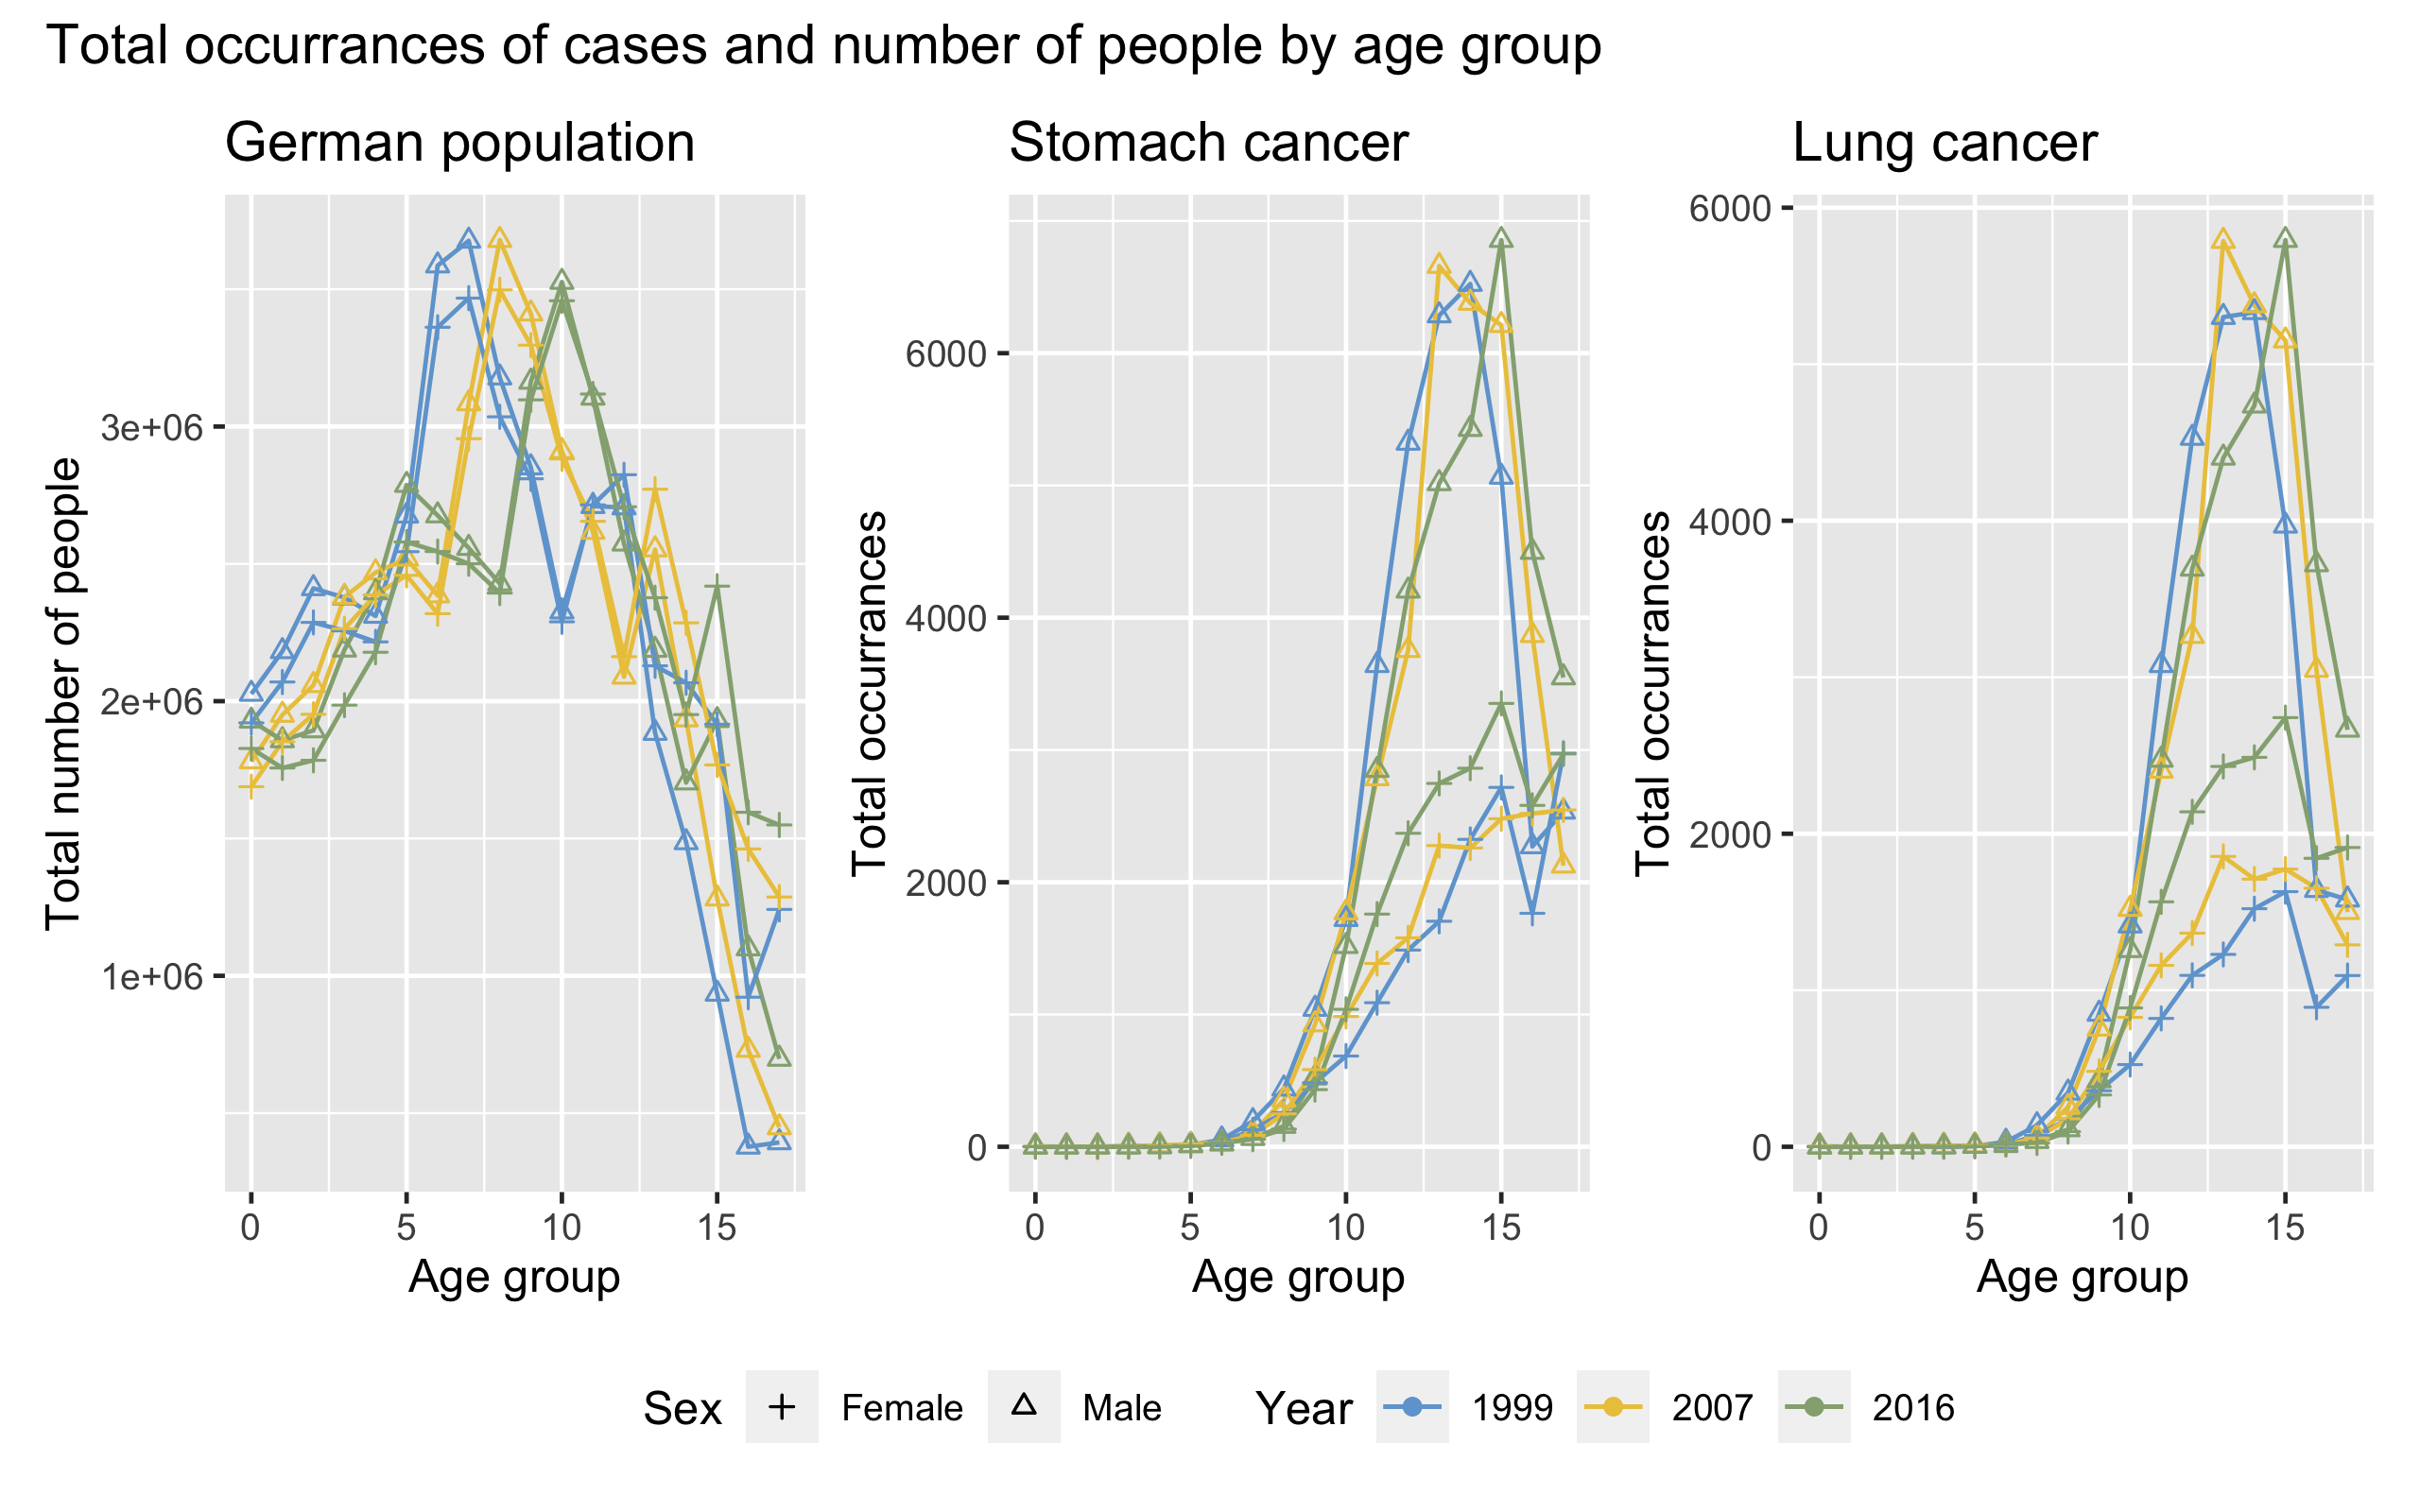
\includegraphics[width=\linewidth]{real-data/real-data-univariate/Figures/data-age-total.png}
    \end{subfigure}
    
    \begin{subfigure}[b]{.6\linewidth}
        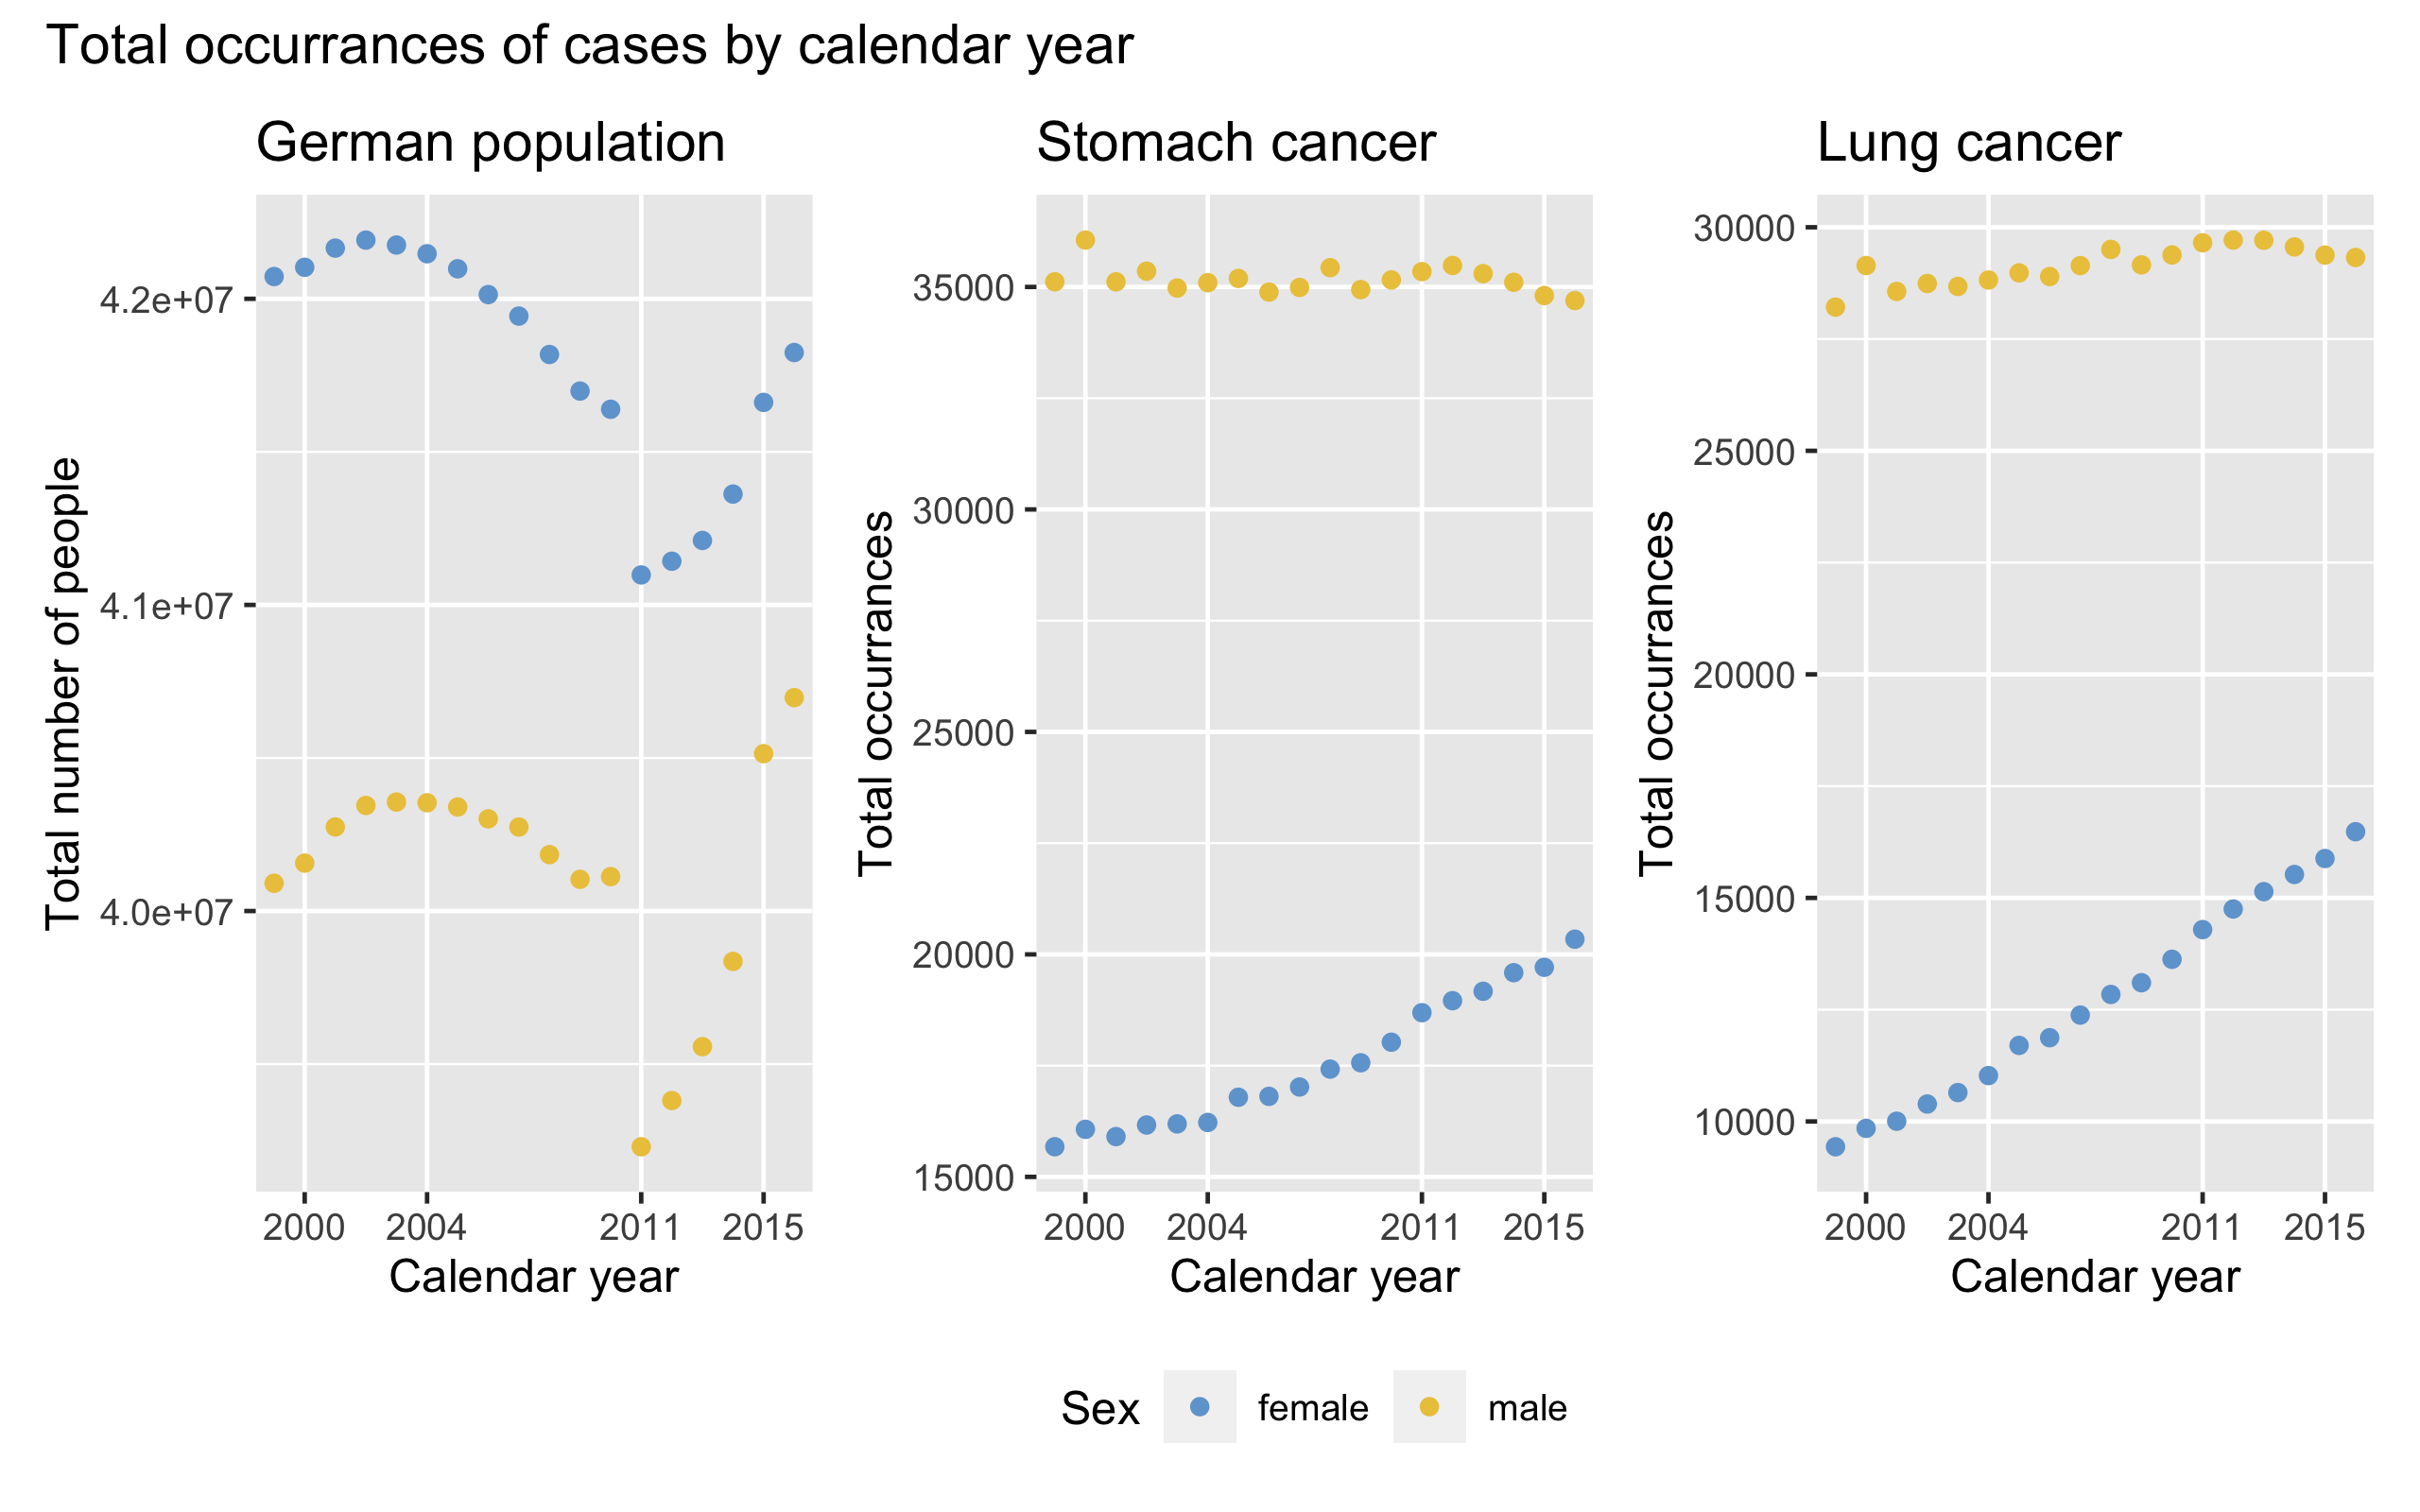
\includegraphics[width=\linewidth]{real-data/real-data-univariate/Figures/data-year-total.png}
    \end{subfigure}
    \caption{The observed population for Germany and the observed cases for lung and stomach cancer deaths. \textit{Left:} The data is summed over all years for each age group. \textit{Right:} The data is summed over all age groups for each year. \texcolor{myDarkBlue}{TODO: Change axis labels.}}
    \label{fig:data-total}
\end{figure}

\newpar Figure \ref{fig:data-rate} present the observed mortality rates for years 1999, 2005, 2011 and 2016, for each age group and cohort. We observe that for younger ages, the mortality rates are close to zero for both lung and stomach cancer. For the years 2005, 2011 and 2016 we see that we do not have observations for the  mortality rates for older cohorts (lower cohort index $k$). On the other side, we see that younger cohorts, at around $k > 60$, have mortality rates that are close to zero for all years. From the left-most part of Figure \ref{fig:data-rate} we see that the male and female mortality rates behave differently over the periods, for both lung ans stomach cancer. As previously indicated, the female mortality rates are in general higher in 2016 compared to 1999, while the opposite is the case for male mortality. This difference is especially apparent for the lung cancer mortality. 

\begin{figure}
    \centering
    \begin{subfigure}[b]{.6\linewidth}
        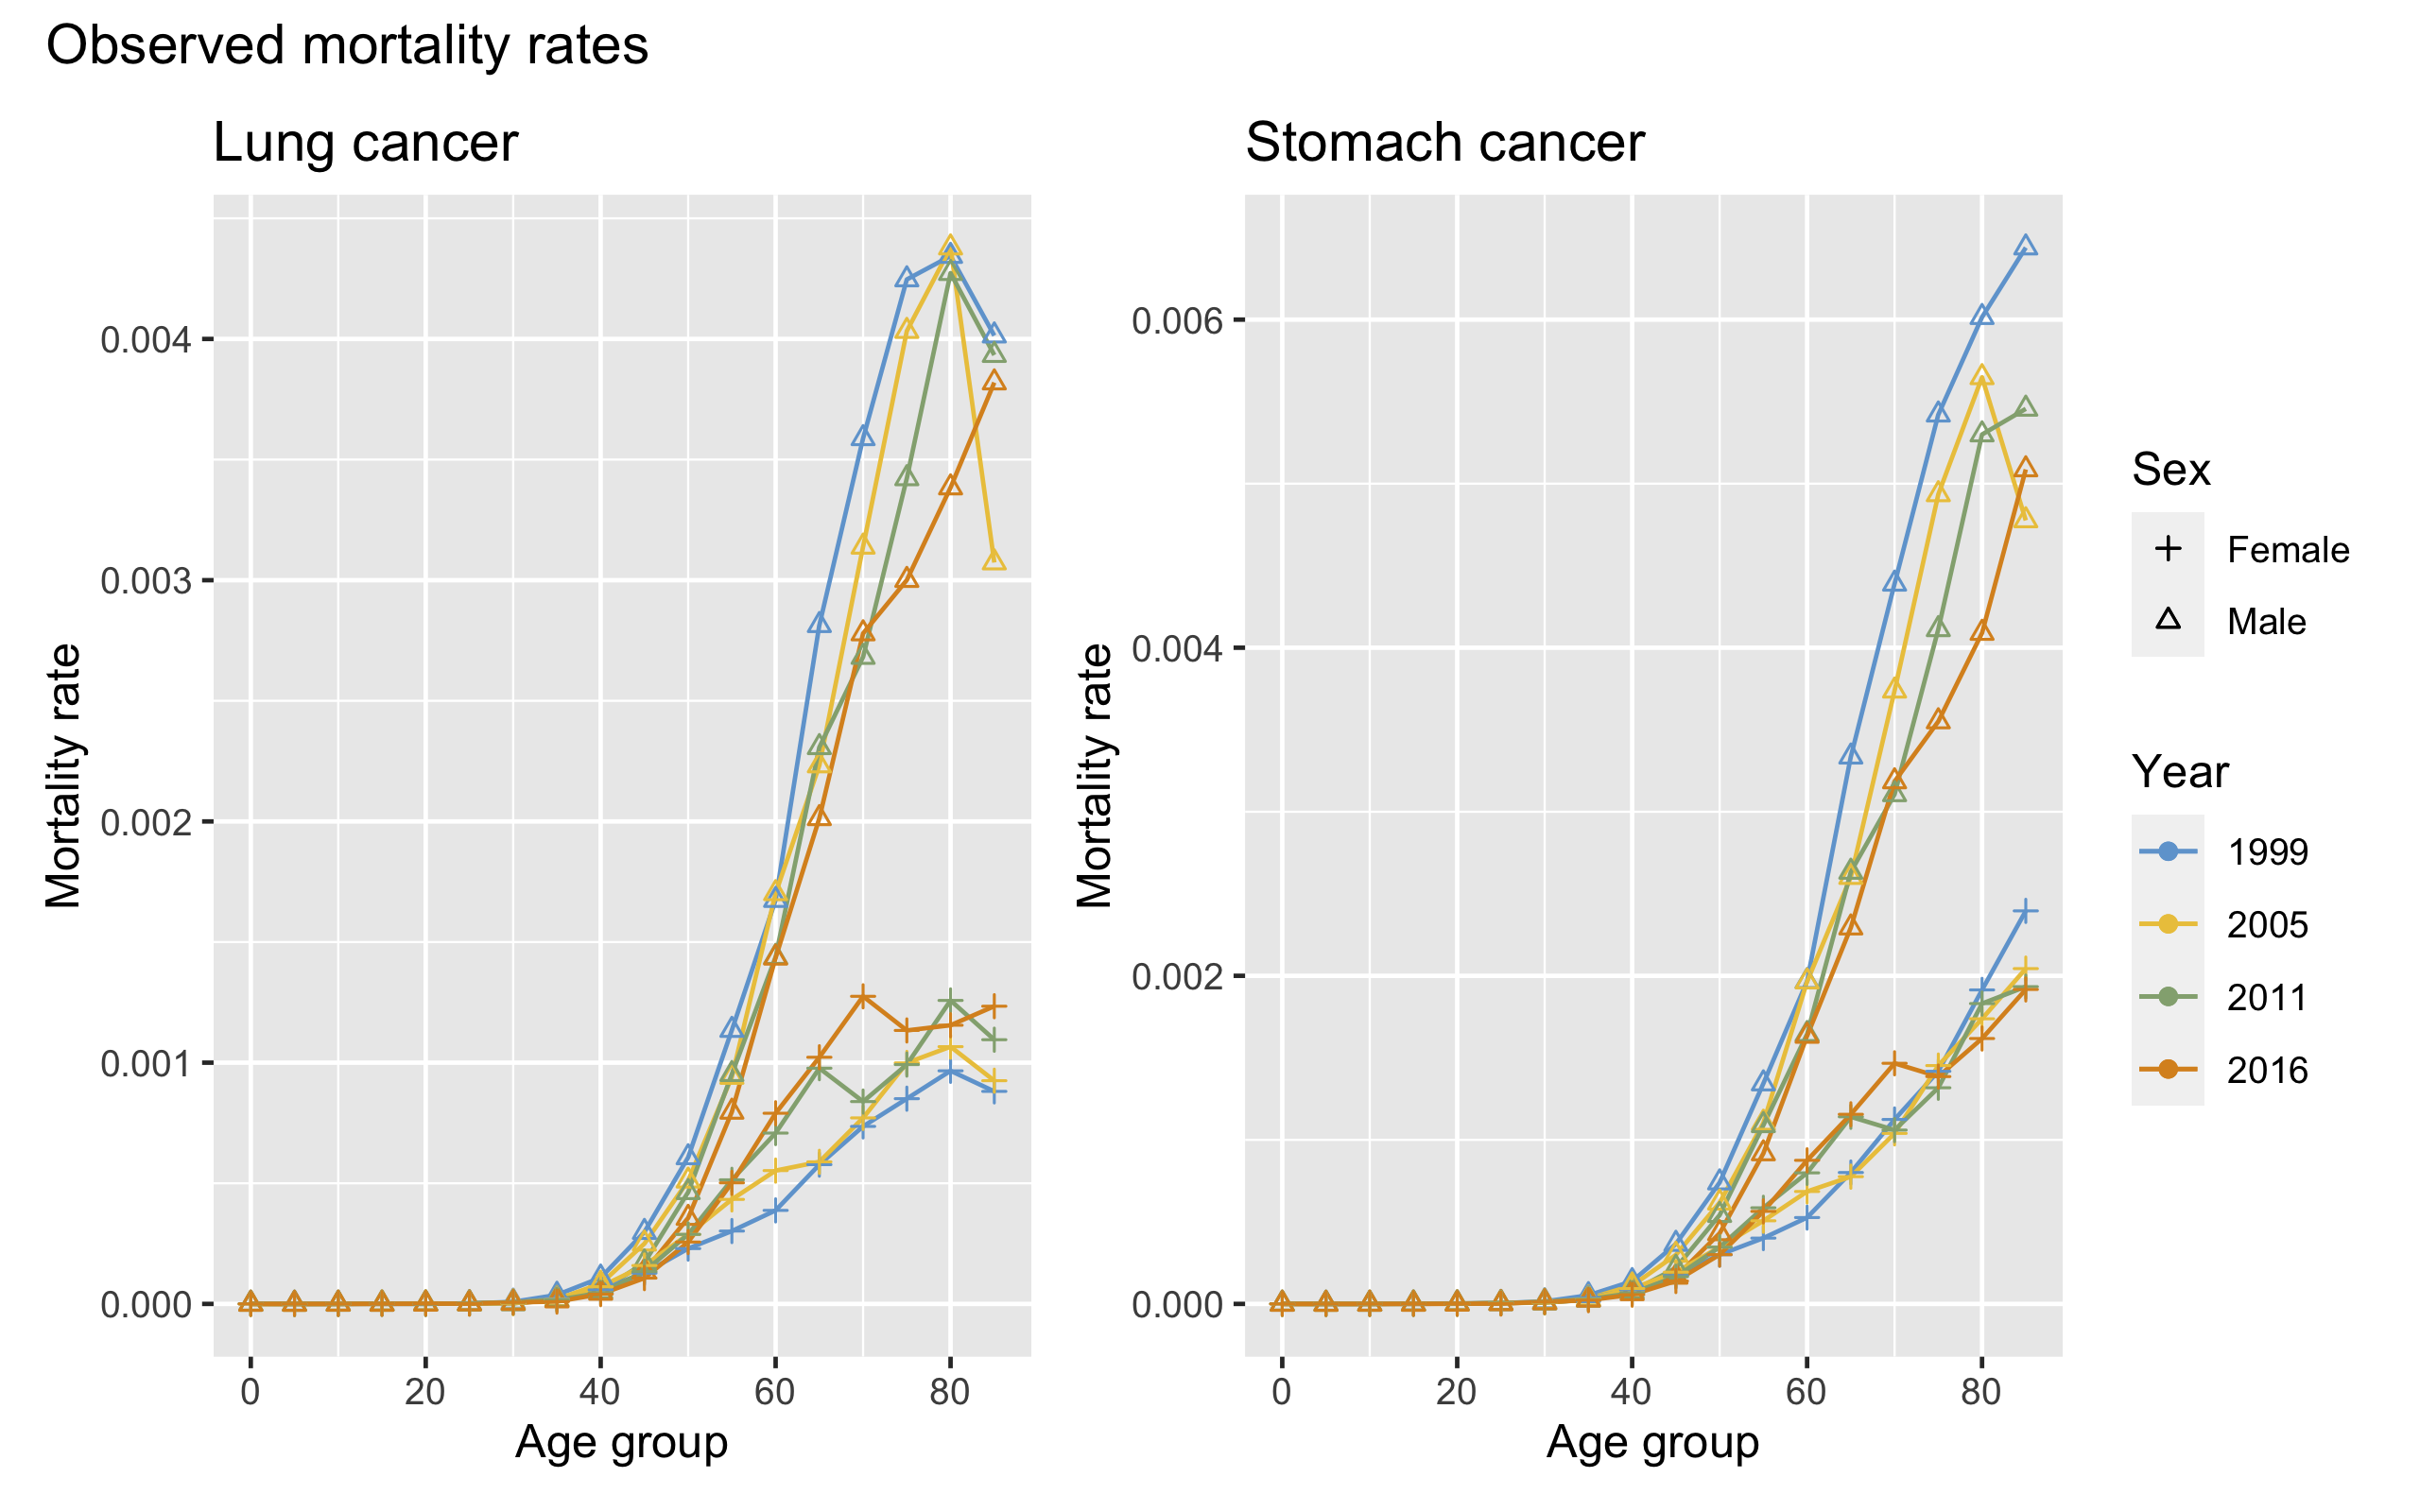
\includegraphics[width=\linewidth]{real-data/real-data-univariate/Figures/data-age-rate.png}
    \end{subfigure}
    
    \begin{subfigure}[b]{.6\linewidth}
        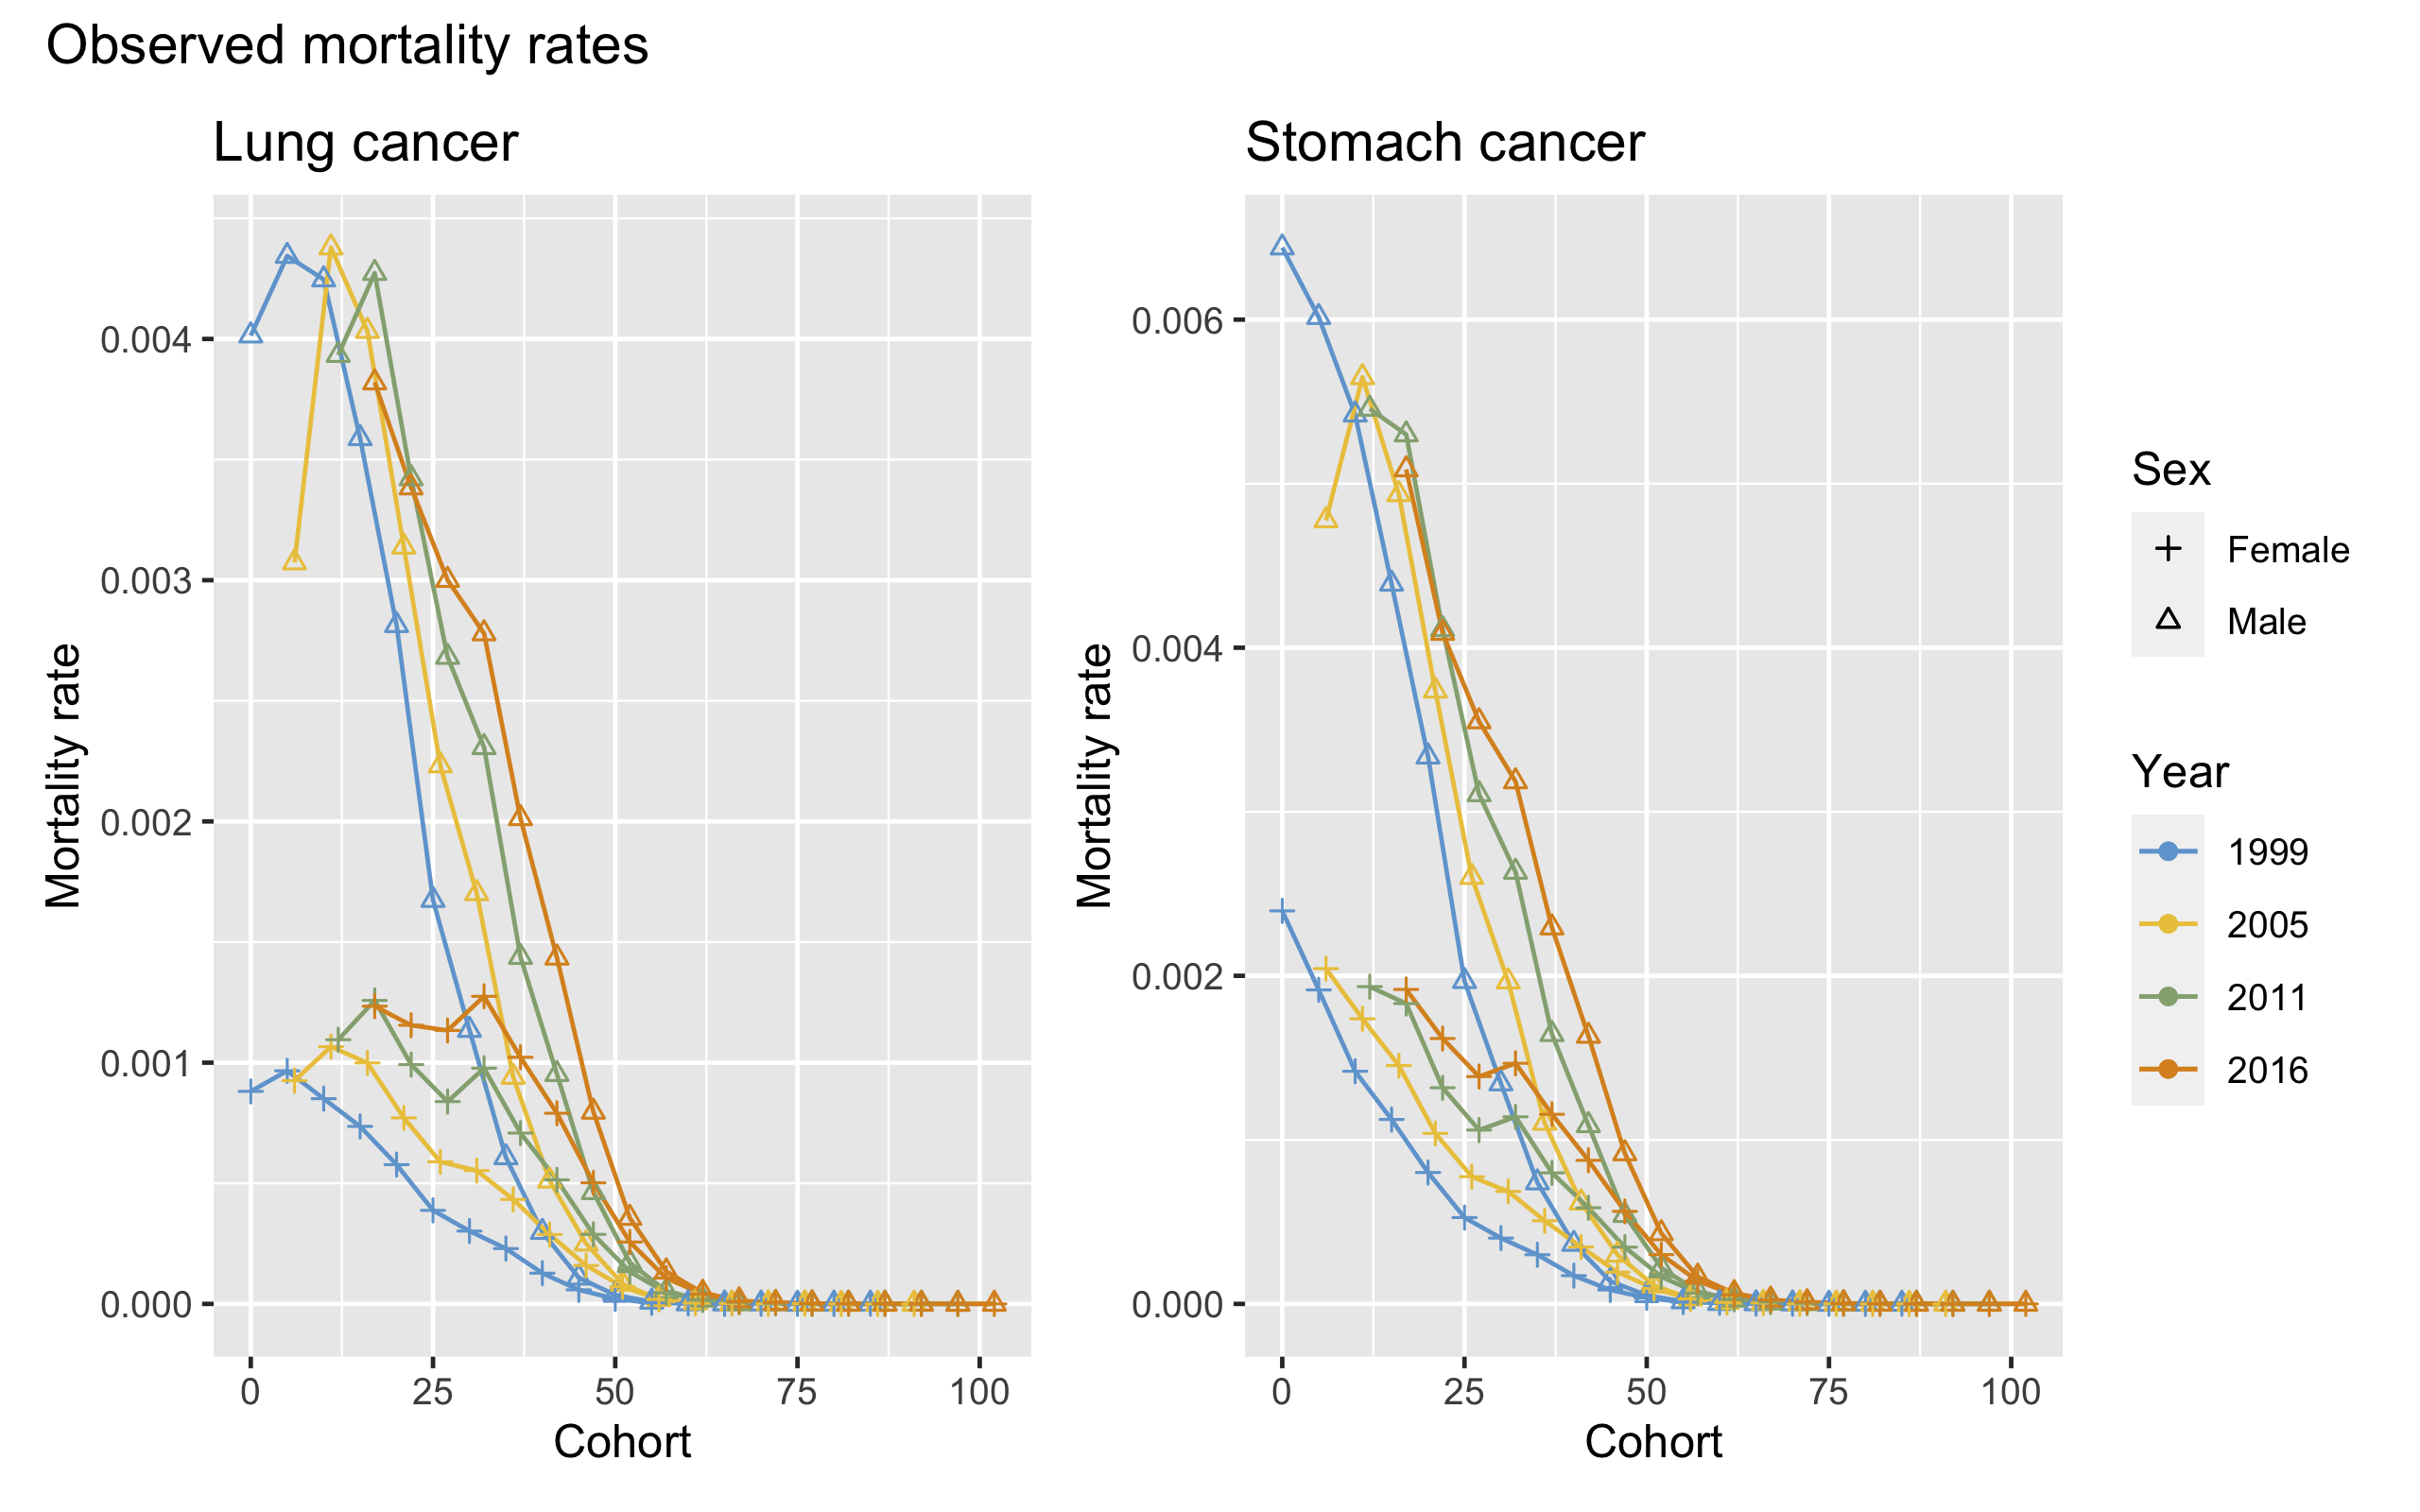
\includegraphics[width=\linewidth]{real-data/real-data-univariate/Figures/data-cohort-rate.png}
    \end{subfigure}
    \caption{The observed mortality rates for the German lung and stomach cancer data, for the years 1999, 2005, 2011 and 2016.}
    \label{fig:data-rate}
\end{figure}

\subsection{Fitting the Lee-Carter Models to the Whole Population}
\label{sec:LC-full-data}
We begin by fitting the Lee-Carter models to the whole population to investigate how estimation with \inlabru behaves when applied to real-life data. We use the same inference procedure as described in Section \ref{sec:implementationInlabru} and the script used to produce the results can be found at 
\path{real-data/real-data-univariate/uv-fit-full-data.R}.

\newpar The resulting estimated effects, as well as the estimated mortality rates, from fitting the LC-model to the lung cancer data are displayed in Figure \ref{fig:uv-full-data-LC-l}. Firstly, we observe, from the lower right plot, that the estimated mortality rates fit well with the observed mortality rates. The value of the intercept is $\approx -9$, corresponding to an overall mortality level at $e^{-9} \sim 10^{-4}$. The age effect $\alpha_x$, has a clear increasing trend, as expected since we have seen, from e.g. Figure \ref{fig:data-rate}, that the lung cancer mortality rates increases with age. The estimated value of $\phi$ is negative, indicating an overall decreasing time trend. As discussed in \ref{sec:GermanCancerData}, this is in line with the observed male mortality rates, but not necessarily the female mortality rates. Furthermore, we observe that the estimated $\beta_x$ have quite wide confidence bounds for younger ages, but with a clear decreasing trend for older ages. Finally, we note that the confidence bounds of $\kappa_t$ are quite wide and centered mostly around zero. This could be an indication that the effect of $\kappa_t$, which we interpret as the variation in the period effect, is not significant. 

\begin{figure}[h!]
    \centering
    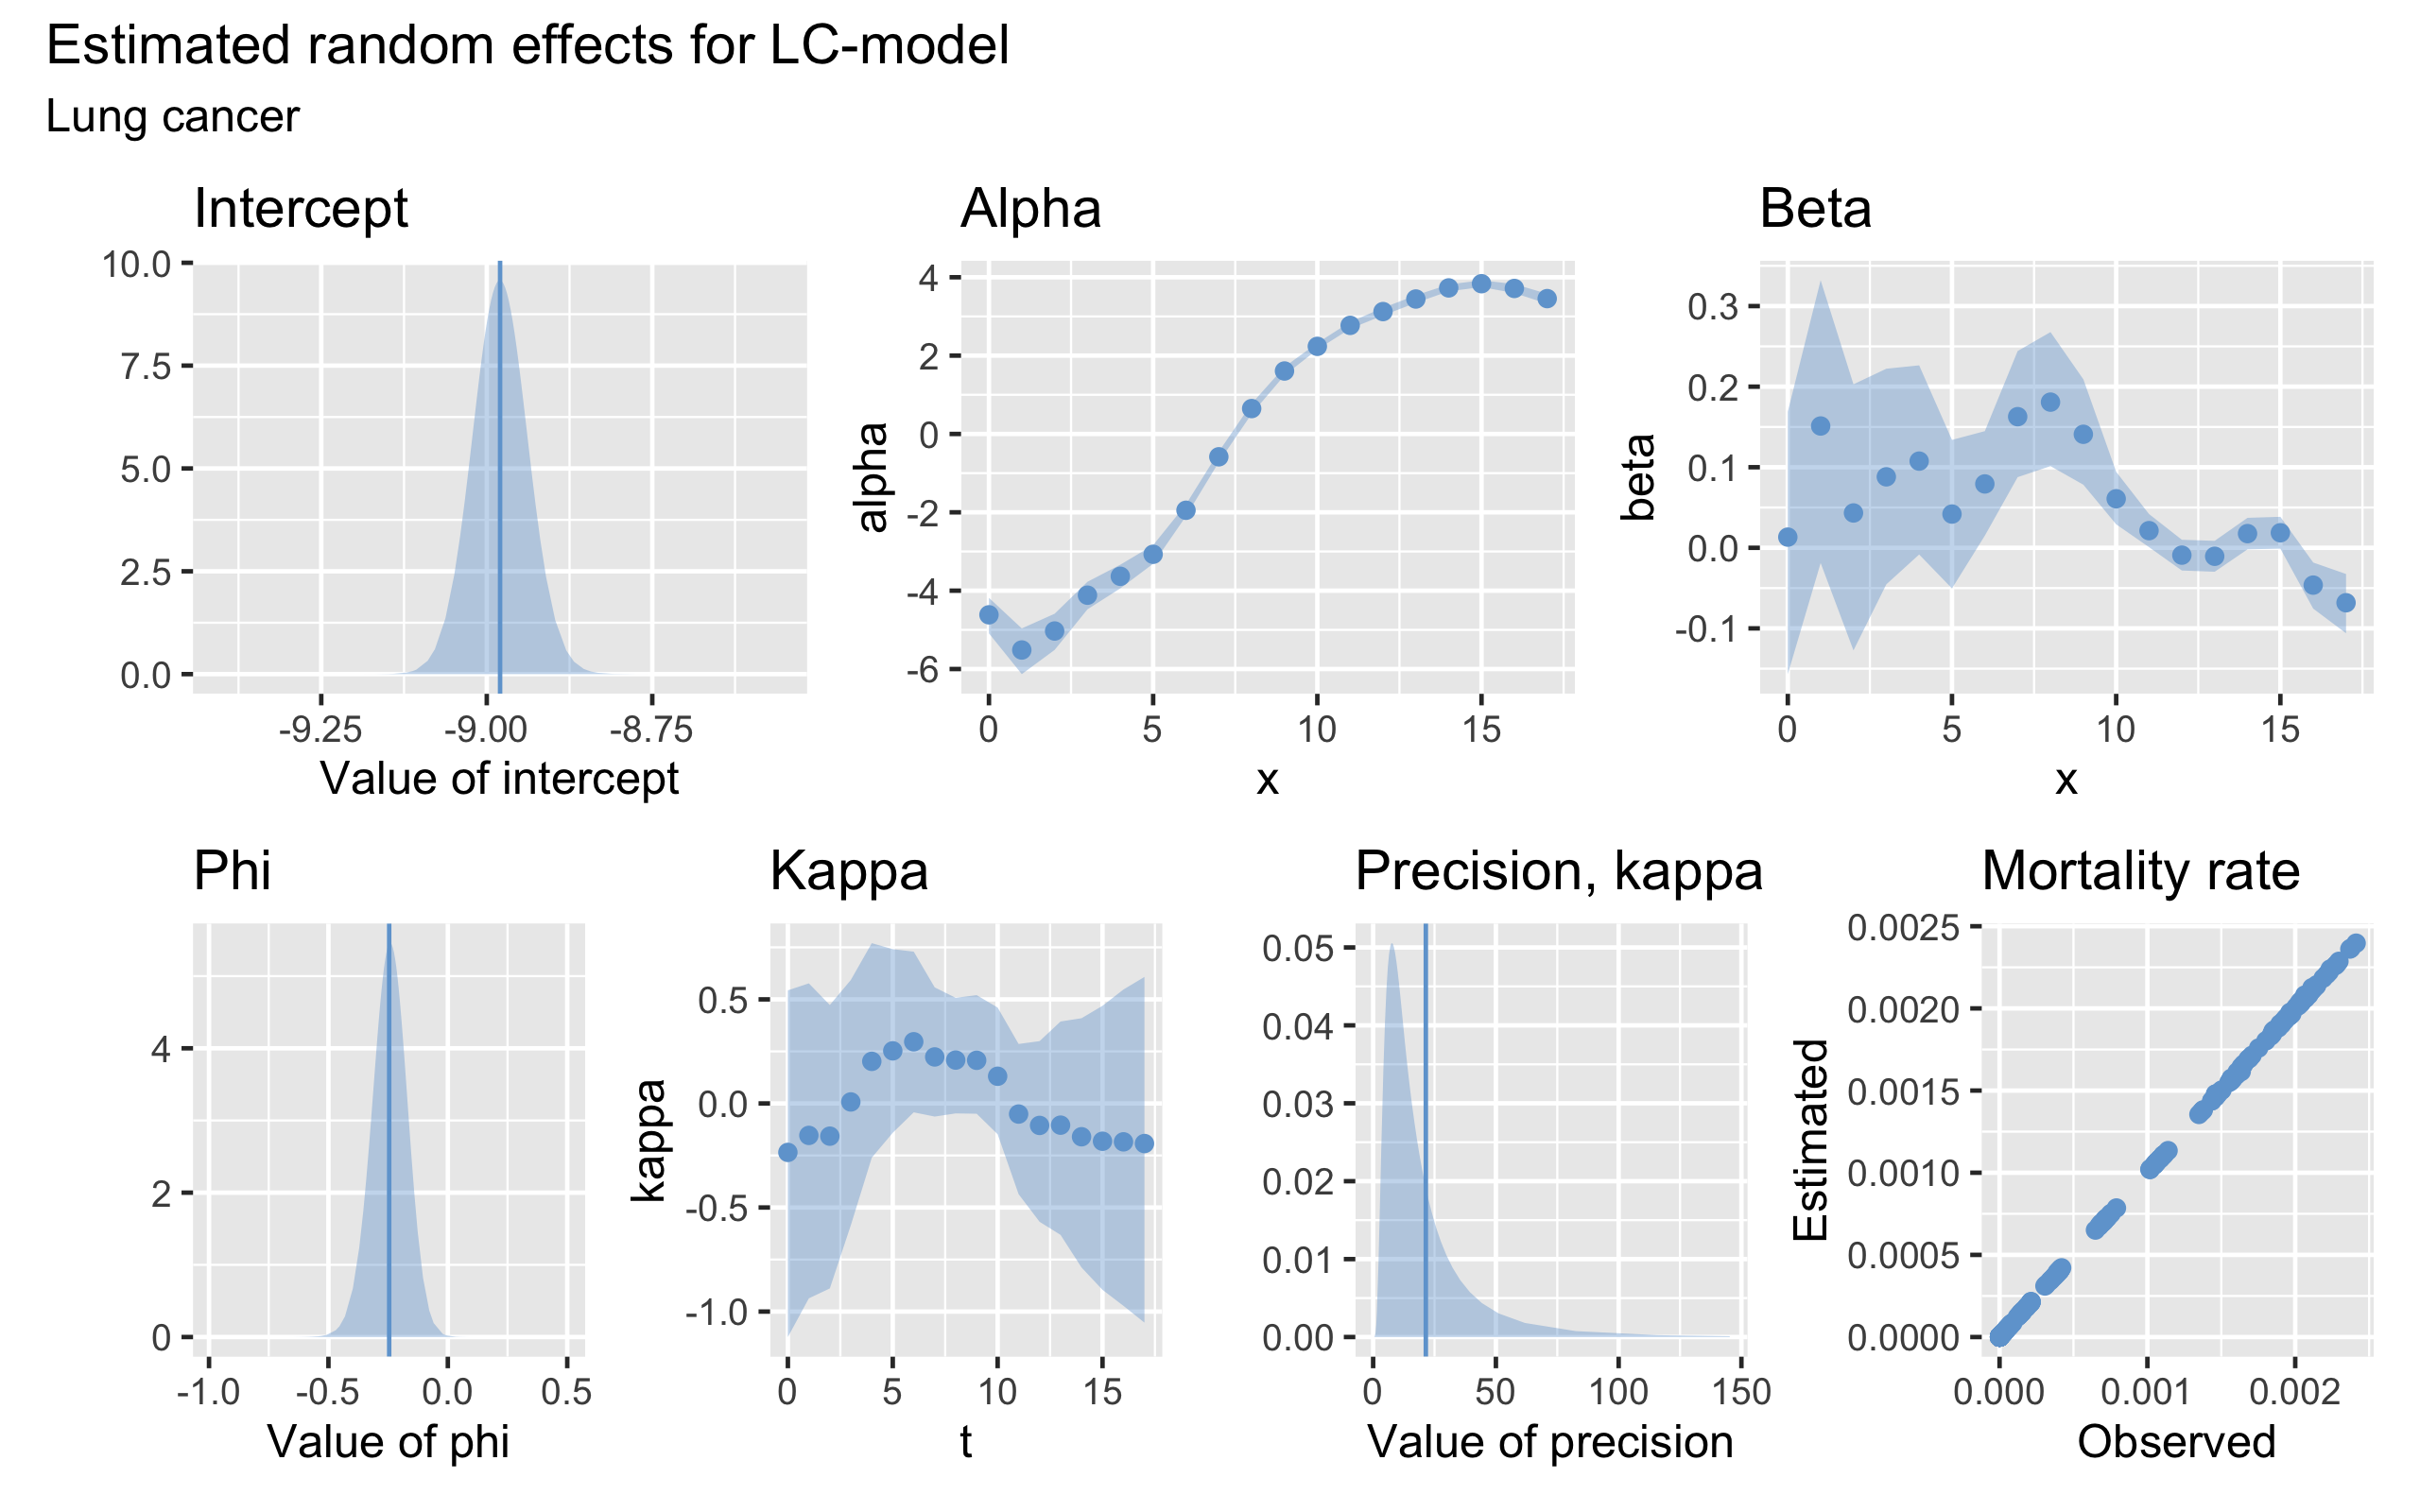
\includegraphics[width=0.85\linewidth]{real-data/real-data-univariate/Figures/uv-full-data-lc-l.png}
    \caption{The estimation results from fitting the LC-model to the lung cancer data. The lower right plot show the estimated mean values of the mortality rates plotted against the observed mortality rates $Y_{x,t}^{\text{lung}}$. The "Precision, kappa" plot the estimated marginal distribution of the precision $\tau_\kappa$ for the period effect $\kappa_t$. The remaining plots display the mean and 95\% confidence bounds of the estimations of the intercept $\mu$ and the random effects $\alpha_x$, $\beta_x$, $\phi$ and $\kappa_t$.}
    \label{fig:uv-full-data-LC-l}
\end{figure}

\newpar The results from fitting the LC-model to the stomach cancer data are quite similar to the lung cancer results, with some minor differences. The plots of these results are included in the Appendix, in Figure \ref{fig:uv-full-data-LC-s}. The estimated values of $\kappa_t$ for stomach cancer seem even less significant than the ones for the lung cancer. Also, the estimated values of $\beta_x$ has a less clear decrease with older ages. 

\begin{figure}[h!]
    \centering
    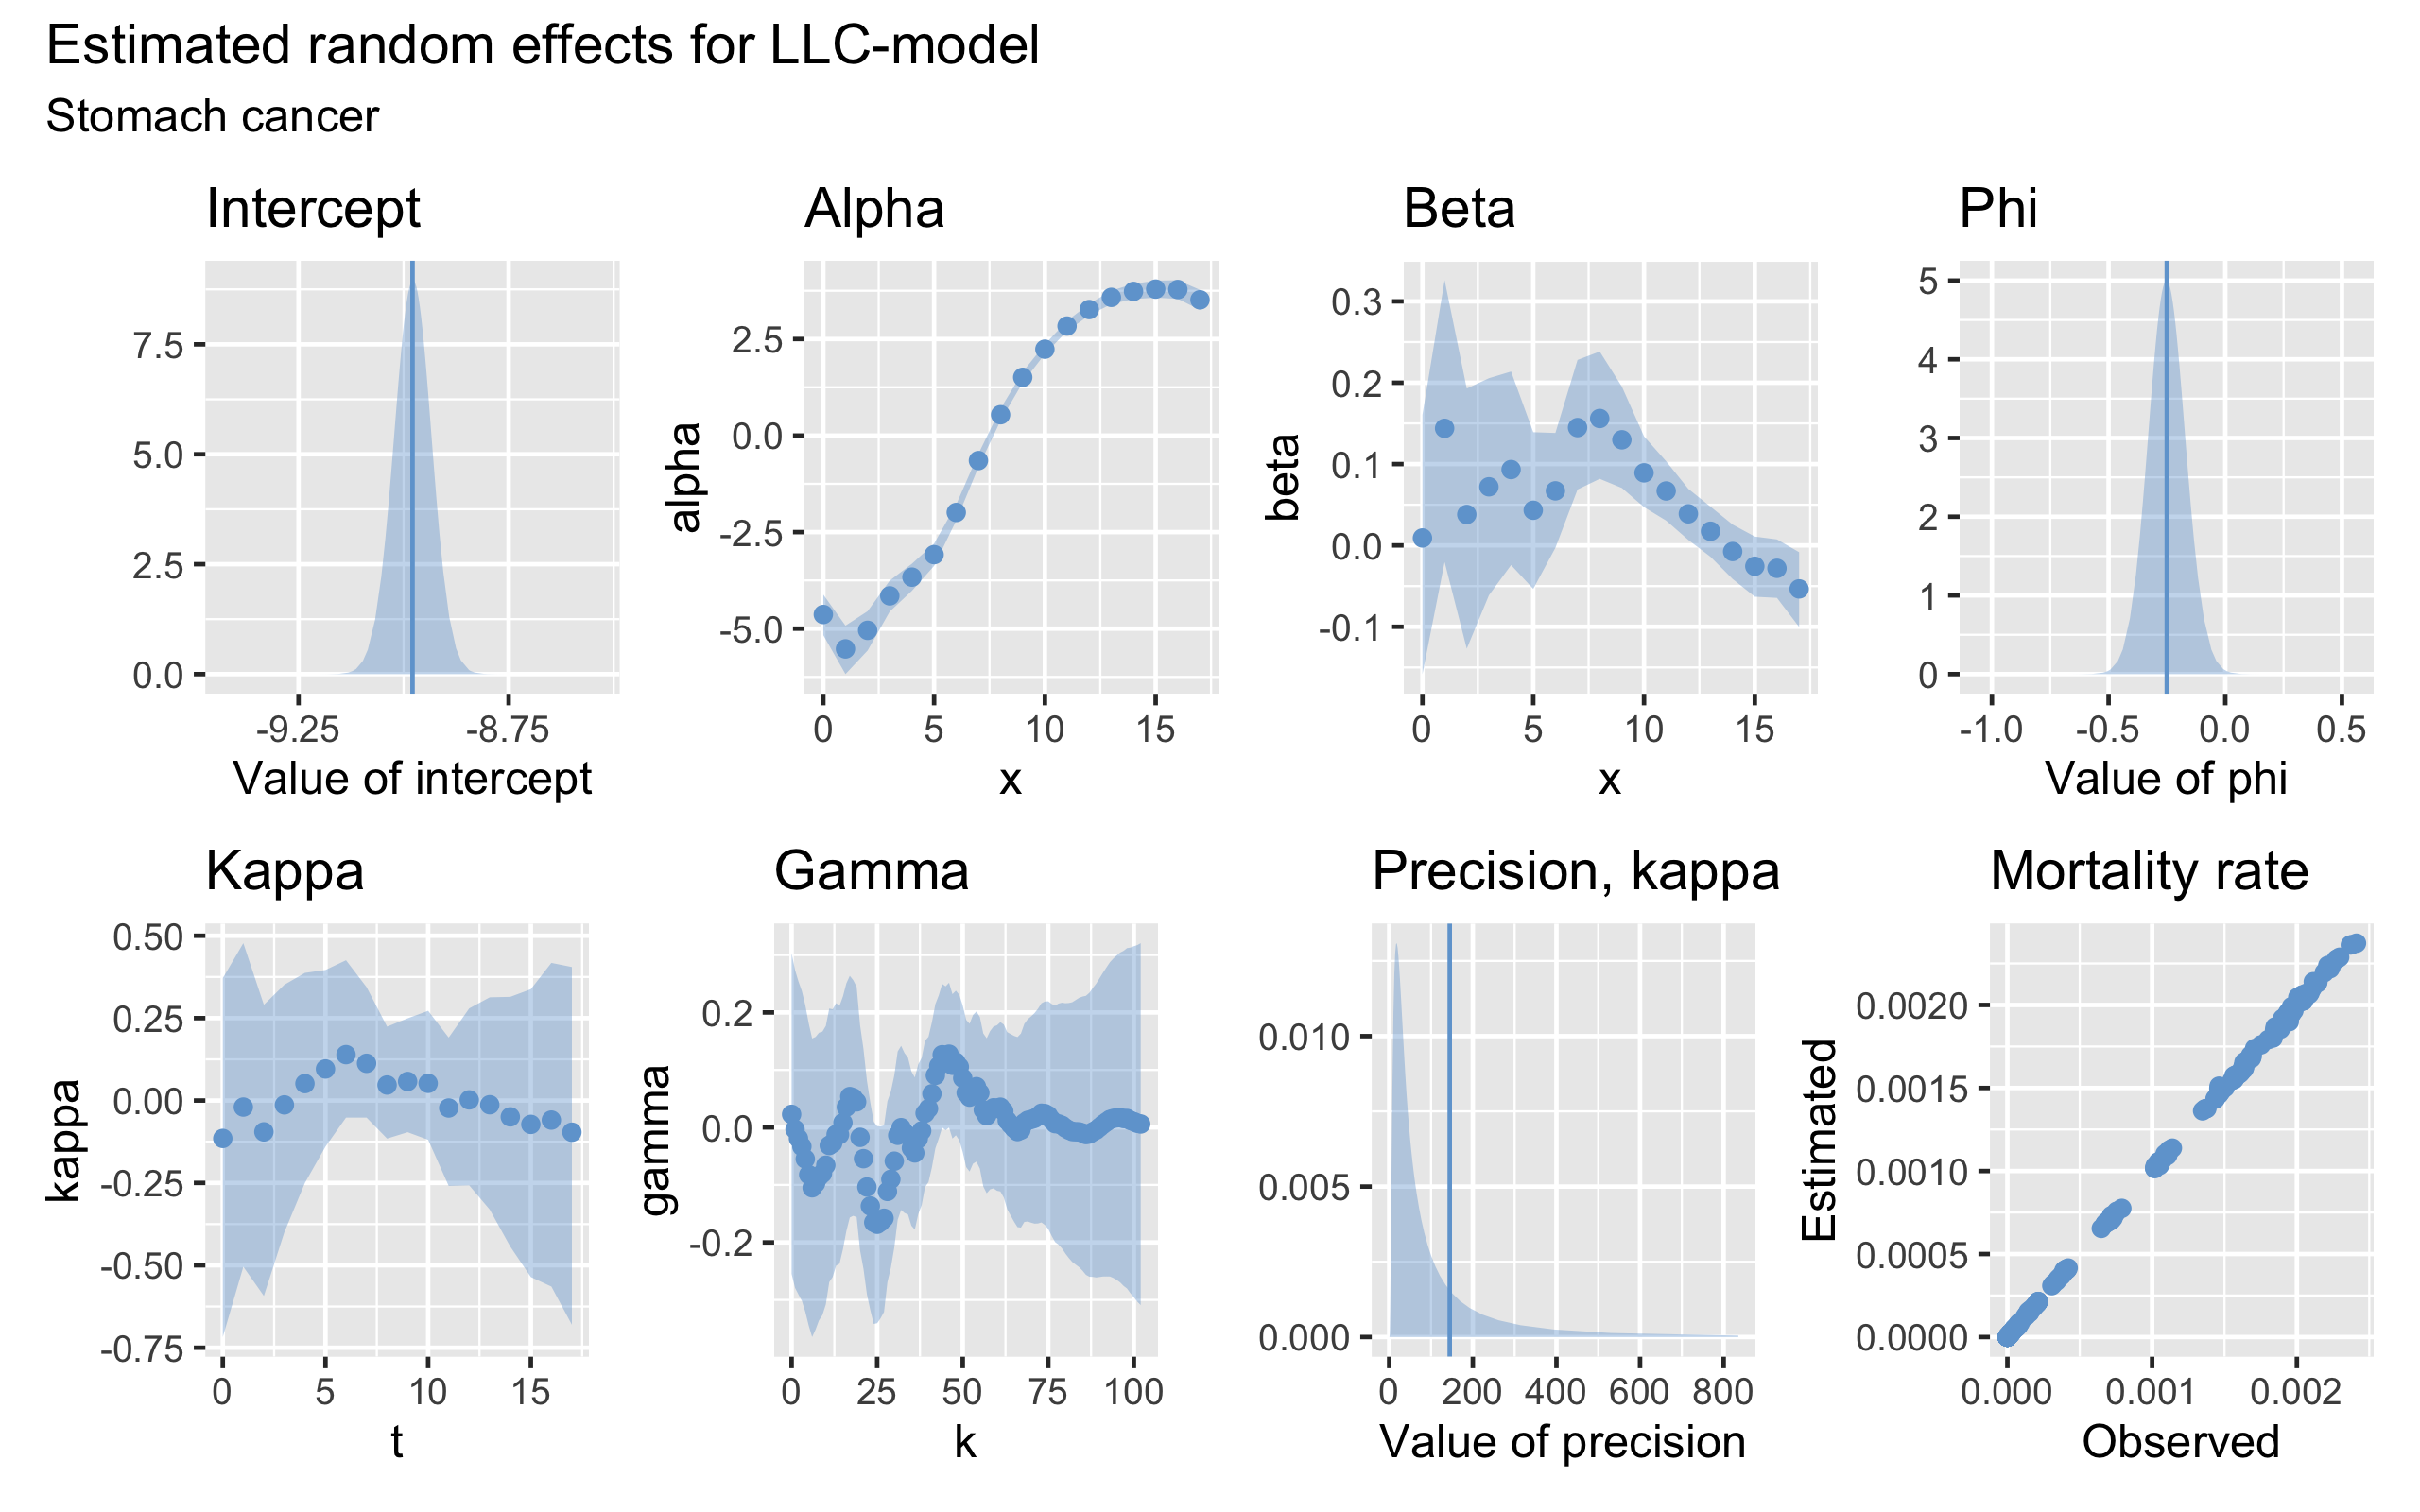
\includegraphics[width=0.85\linewidth]{real-data/real-data-univariate/Figures/uv-full-data-lcc-l.png}
    \caption{The estimation results from fitting the LCC-model to the lung cancer data. The layout of the plots is similar to that of Figure \ref{fig:uv-full-data-LC-l}, with an inclusion of the estimated cohort effect $\gamma_k$.}
    \label{fig:uv-full-data-LCC-l}
\end{figure}

\newpar The results from fitting the LCC-model to lung cancer data are displayed in Figure \ref{fig:uv-full-data-LCC-l}. It should be noted that \inlabru uses more than 50 iterations to converge for this case, and so the result presented here is the value found after 50 runs. This in an indication that finding an optimal linearization point for the LCC-model for the lung cancer data is difficult. Since the estimated mortality rates seem to fit well with the observed mortality rates, we choose to not discard the LCC-model for the lung cancer data because of this. The trends of the estimated values for the intercept, $\phi$, $\alpha_x$, $\beta_x$ and $\kappa_t$ are quite similar to that of the LC-model. We observe that there is large variations in the estimated values for the cohort effect $\gamma_k$, with a peak at around $k = 50$ (corresponding to birth years around 1960). \textcite{RieblerThesis2010} have discussed similar periodicity in the cohort effect in APC-models, that arise from unidentifiability when the age- and period-intervals are of different lengths. Since we observe strong similarities between the nature of the identifiability issues described by \textcite{RieblerThesis2010} and the estimated cohort effects here, we treat this result with some scepticism. We do then not conclude that the variability in the estimated cohort effects capture actual cohort-specific variability in lung cancer mortality rates. 

\begin{figure}[h!]
    \centering
    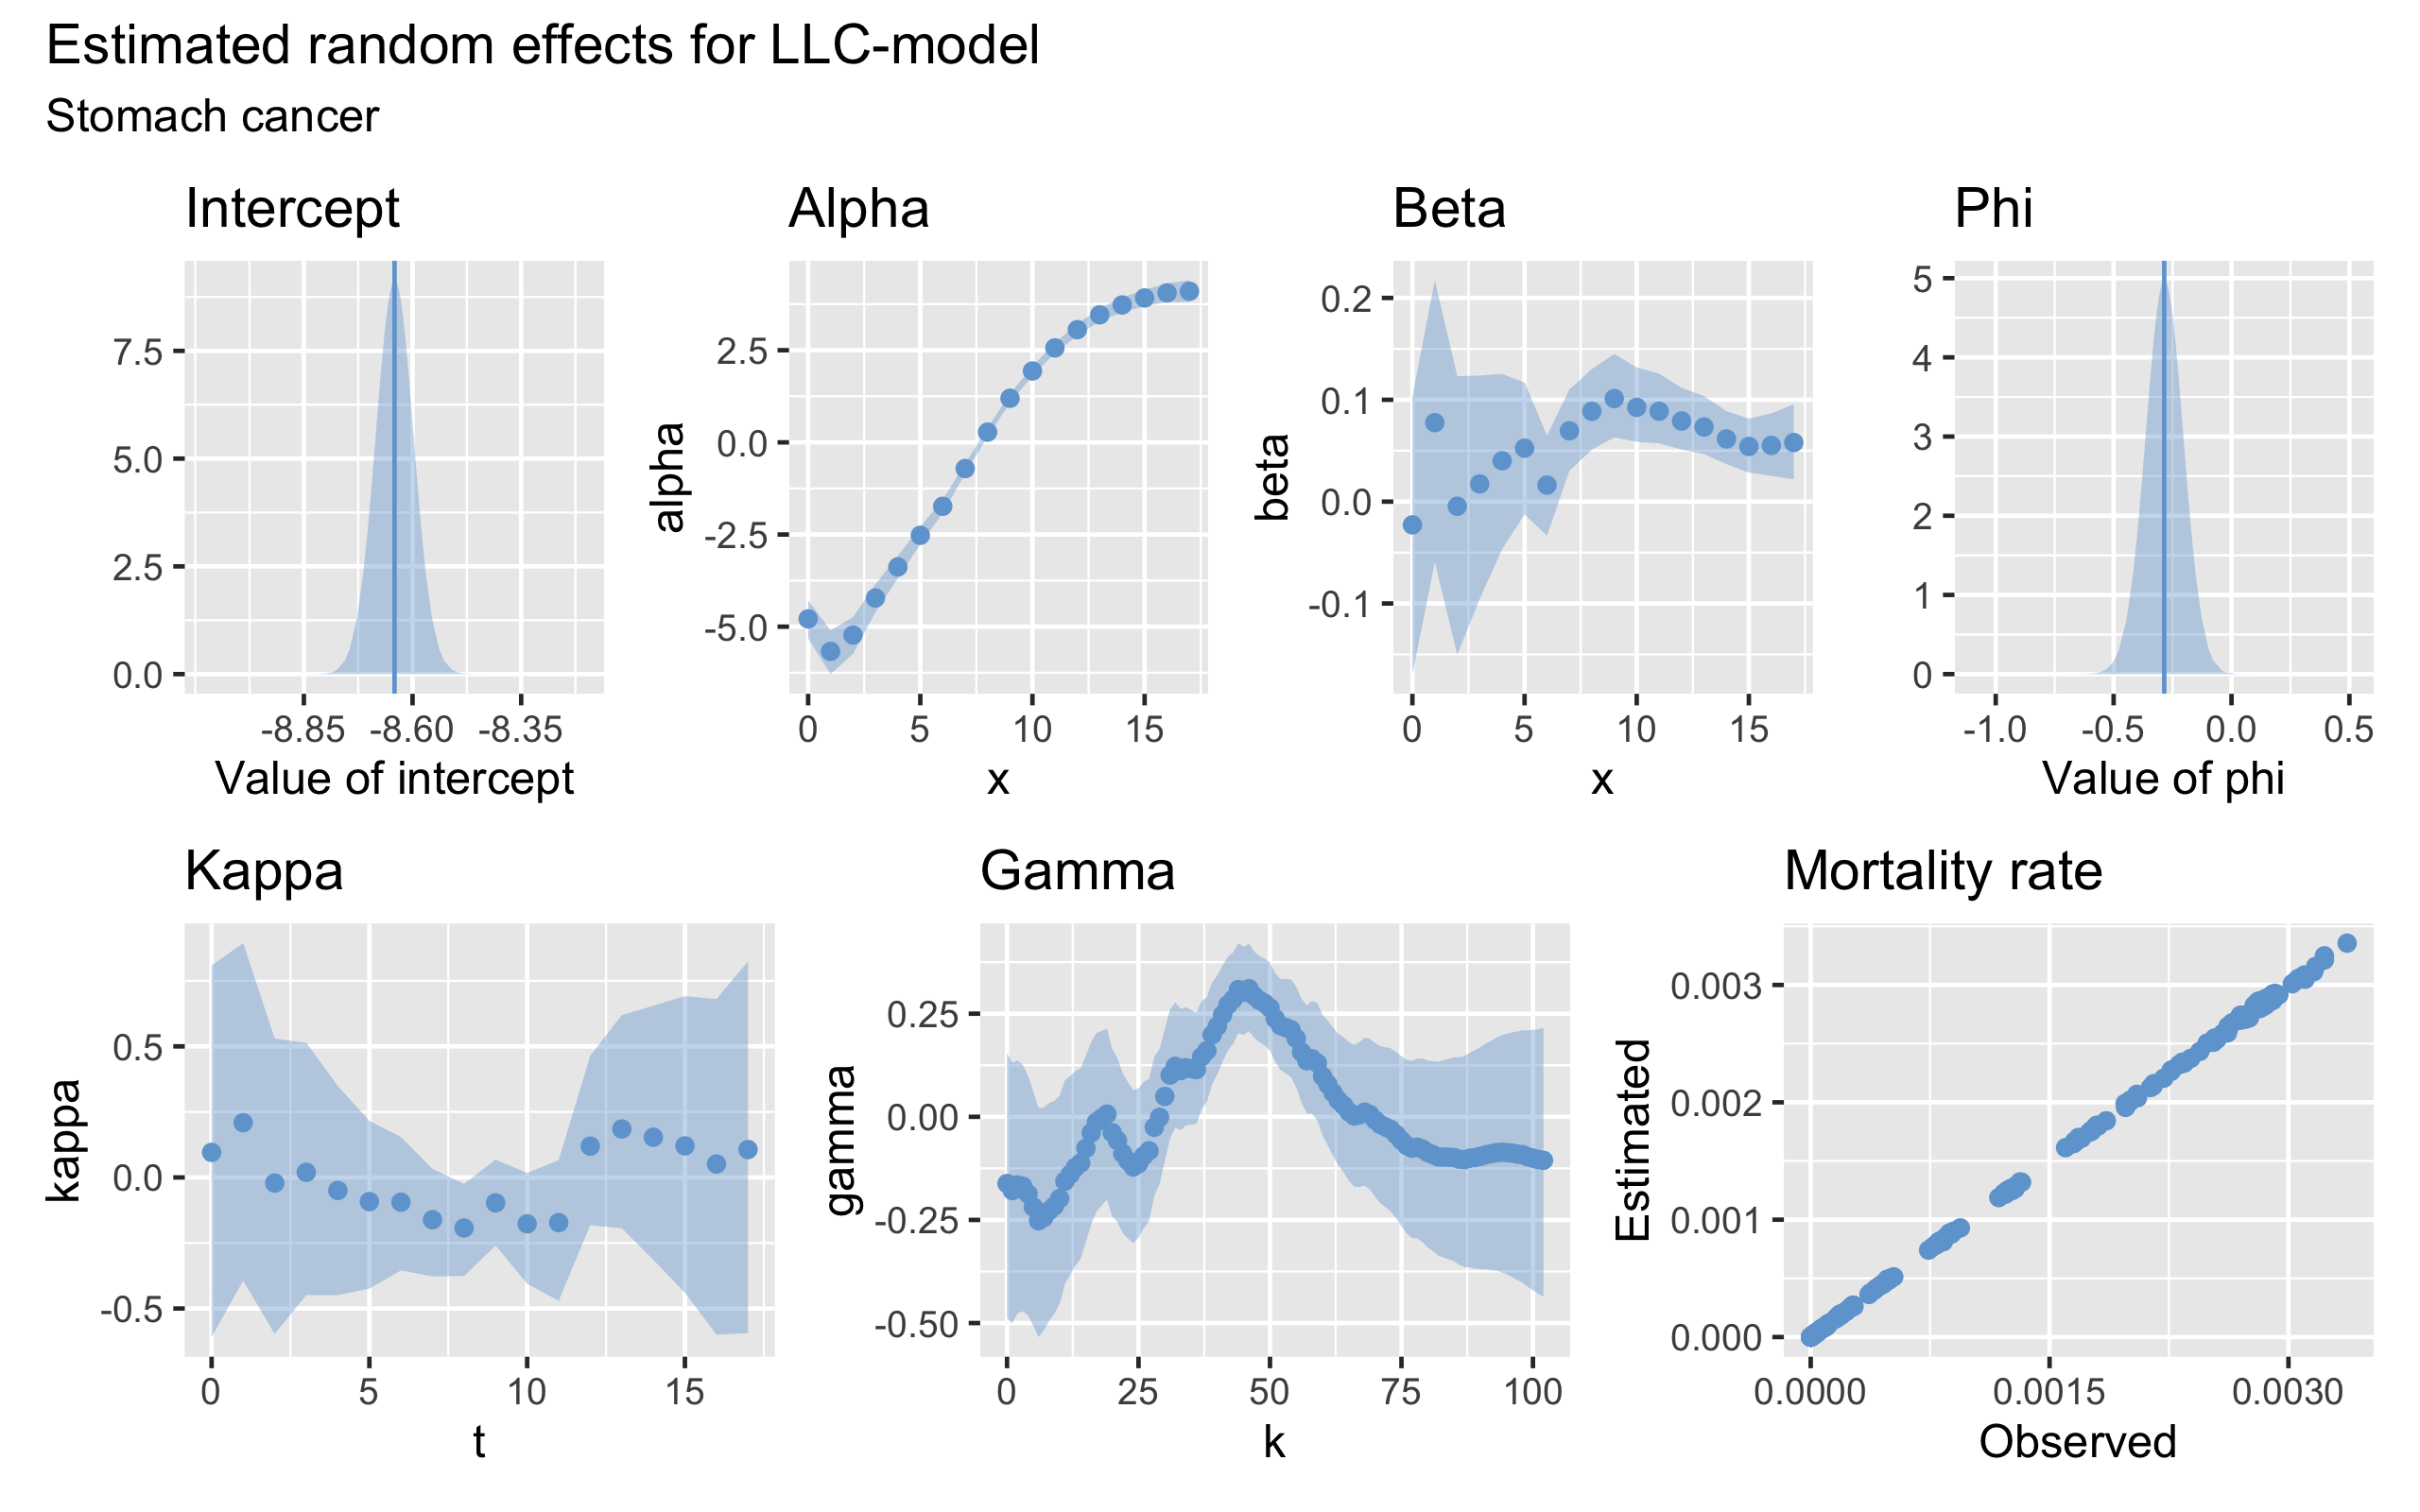
\includegraphics[width=0.85\linewidth]{real-data/real-data-univariate/Figures/uv-full-data-lcc-s.png}
    \caption{The estimation results from fitting the LCC-model to the stomach cancer data. The layout of the plots is similar to that of Figure \ref{fig:uv-full-data-LC-l}, with an inclusion of the estimated cohort effect $\gamma_k$.}
    \label{fig:uv-full-data-LCC-s}
\end{figure}

\newpar The results from fitting the LCC-model to stomach cancer data are displayed in Figure \ref{fig:uv-full-data-LCC-s}. The overall results are quite similar to the previously discussed results. We observe some variability in $\gamma_k$, similar to the one discussed for the lung-cancer estimations, but to a lesser degree. For stomach cancer as well, $\gamma_k$ has a peak at around $k = 50$. Additionally, we observe a difference in the trend of $\beta_x$ compared for the estimated $\beta_x$ for lung cancer, as it decreases much less with age. We observe this tendency when comparing the LC-model fits for the two cancer types as well, but to a lesser degree. Recalling that $\beta_x$ can be interpreted as the age-specific sensitivity to period-related change in mortality, we interpret this as an indication of larger period-related differences in cancer mortality for older age groups in stomach cancer compared to lung cancer. We finally note that for lung cancer, some values of $\beta_x$ are less than zero for the oldest age groups (this can be seen in Figures \ref{fig:uv-full-data-LC-l} and \ref{fig:uv-full-data-LCC-l}). These negative values of $\beta_x$ will then change the sign of the period effects, indicating an increase in mortality rates over time for the oldest age groups. 

% To get an overview of the dataset and the performance of the LC model on these datasets, we begin by fitting the LC and the LCC model to the full datasets and compare it to plots of the data. 

% \newpar Figures \ref{fig:data-by-age}, \ref{fig:data-by-year} and \ref{fig:data-by-cohort} display percent-wise deaths by lung - and stomach cancer, by age groups, years and cohorts (birth years) respectively. Figure \ref{fig:LC-full-dataset} display the random effects obtained by fitting the LC-model to the two data sets, as well as the estimated predictor. Figure \ref{fig:LCC-full-dataset} displays the results from fitting the LCC-model to the stomach cancer data set. 

% \newpar From the Figure \ref{fig:LC-full-dataset} and Figure \ref{fig:LCC-full-dataset} we see that $\alphav$ is the random effect that is modeled with the highest precision for both the LC-model and the LCC-model. This indicates a clear tendency of change in the mortality rate for different age groups, with a higher mortality rate for older age groups. Figure \ref{fig:data-by-age} confirms this, as it shows a much higher mortality rate for older age groups, for both males and females. 
% \newpar We observe from Figures \ref{fig:LC-full-dataset} and \ref{fig:LCC-full-dataset} that there is much higher uncertainty related to the estimation of the period effects, $\kappav$ and $\phi\cdot t$. The estimated $\kappav$ seemes in both cases to be almost insignificant, with wide confidence bounds centered around zero. The $\phi \cdot t$ effect on the other hand, does show a clear tendency of a decreasing mortality rate for higher years.  We also observe a clear tendency in the cohort-effects. 

\subsection{Prediction in the Univariate Case}
\label{sec:uv-pred}
We now compare prediction results for the univariate LC- and LCC-models (see Equations \ref{eq:LC-rewritten} and \ref{eq:LCC-rewritten}) to prediction results for the APC1- and APC2-models (see Section \ref{sec:BayesianInferenceAPC}). Due to the possible insignificance of the $\kappa_t$ effect observed in the previous section, we include an additional version of the LCC-model, where we omit the $\beta_x\cdot \kappa_t$ term, which gives the predictor
\begin{equation}
    \eta_{x,t} = \mu + \alpha_x + \beta_x\cdot \phi \cdot t + \gamma_k + \epsilon_{x,t}.
\end{equation}
We refer to this model as the LCC-linear model, since it only has a linear period term $\phi \cdot t$. By including this model, we can investigate if a reduced version of the model performs better. The code used to produce these results can be found in the \texttt{GitHub} repostitory, under \texttt{real-data/real-data-univariate/predict-long-term.R}. 

\begin{figure}[h!]
    \centering
    \begin{subfigure}[b]{.75\linewidth}
        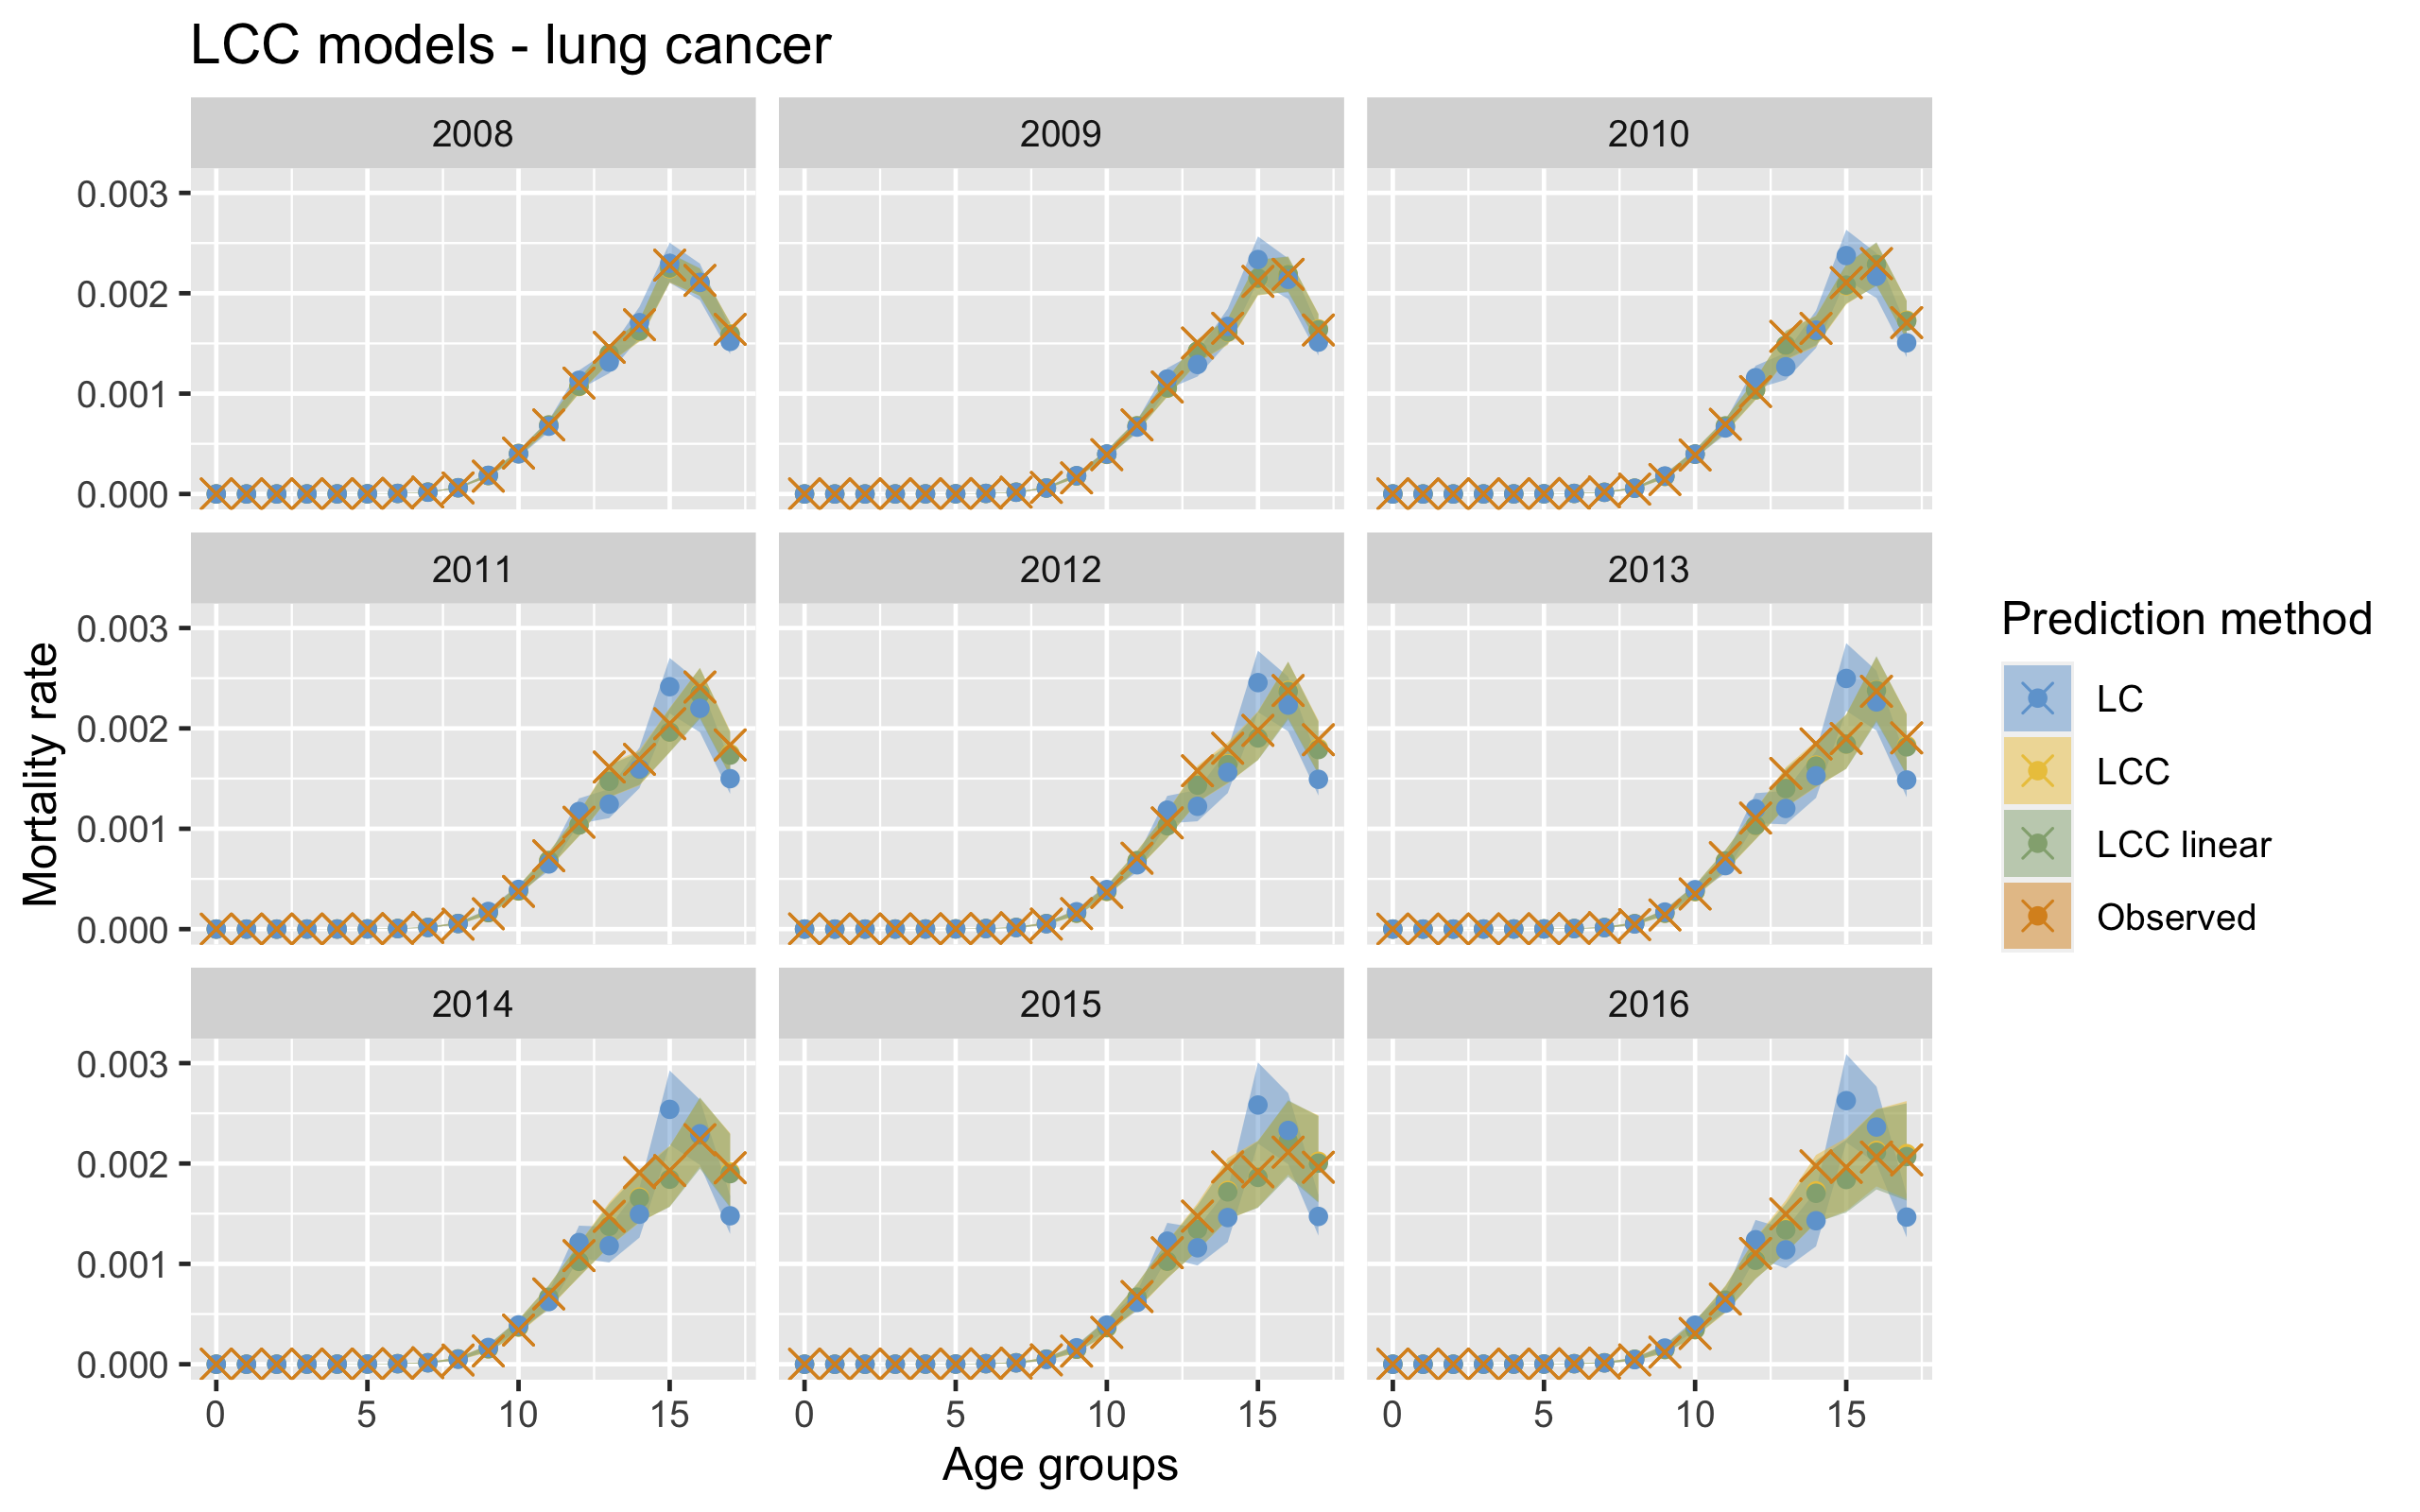
\includegraphics[width=\linewidth]{real-data/real-data-univariate/Figures/univariate-LCC-by-age-lung.png}
        \caption{The prediction results plotted for each of the years that were predicted, with the age groups along the horizontal axis.}
        \label{fig:uv-LCC-lung-top}
    \end{subfigure}
    
    \begin{subfigure}[b]{.75\linewidth}
        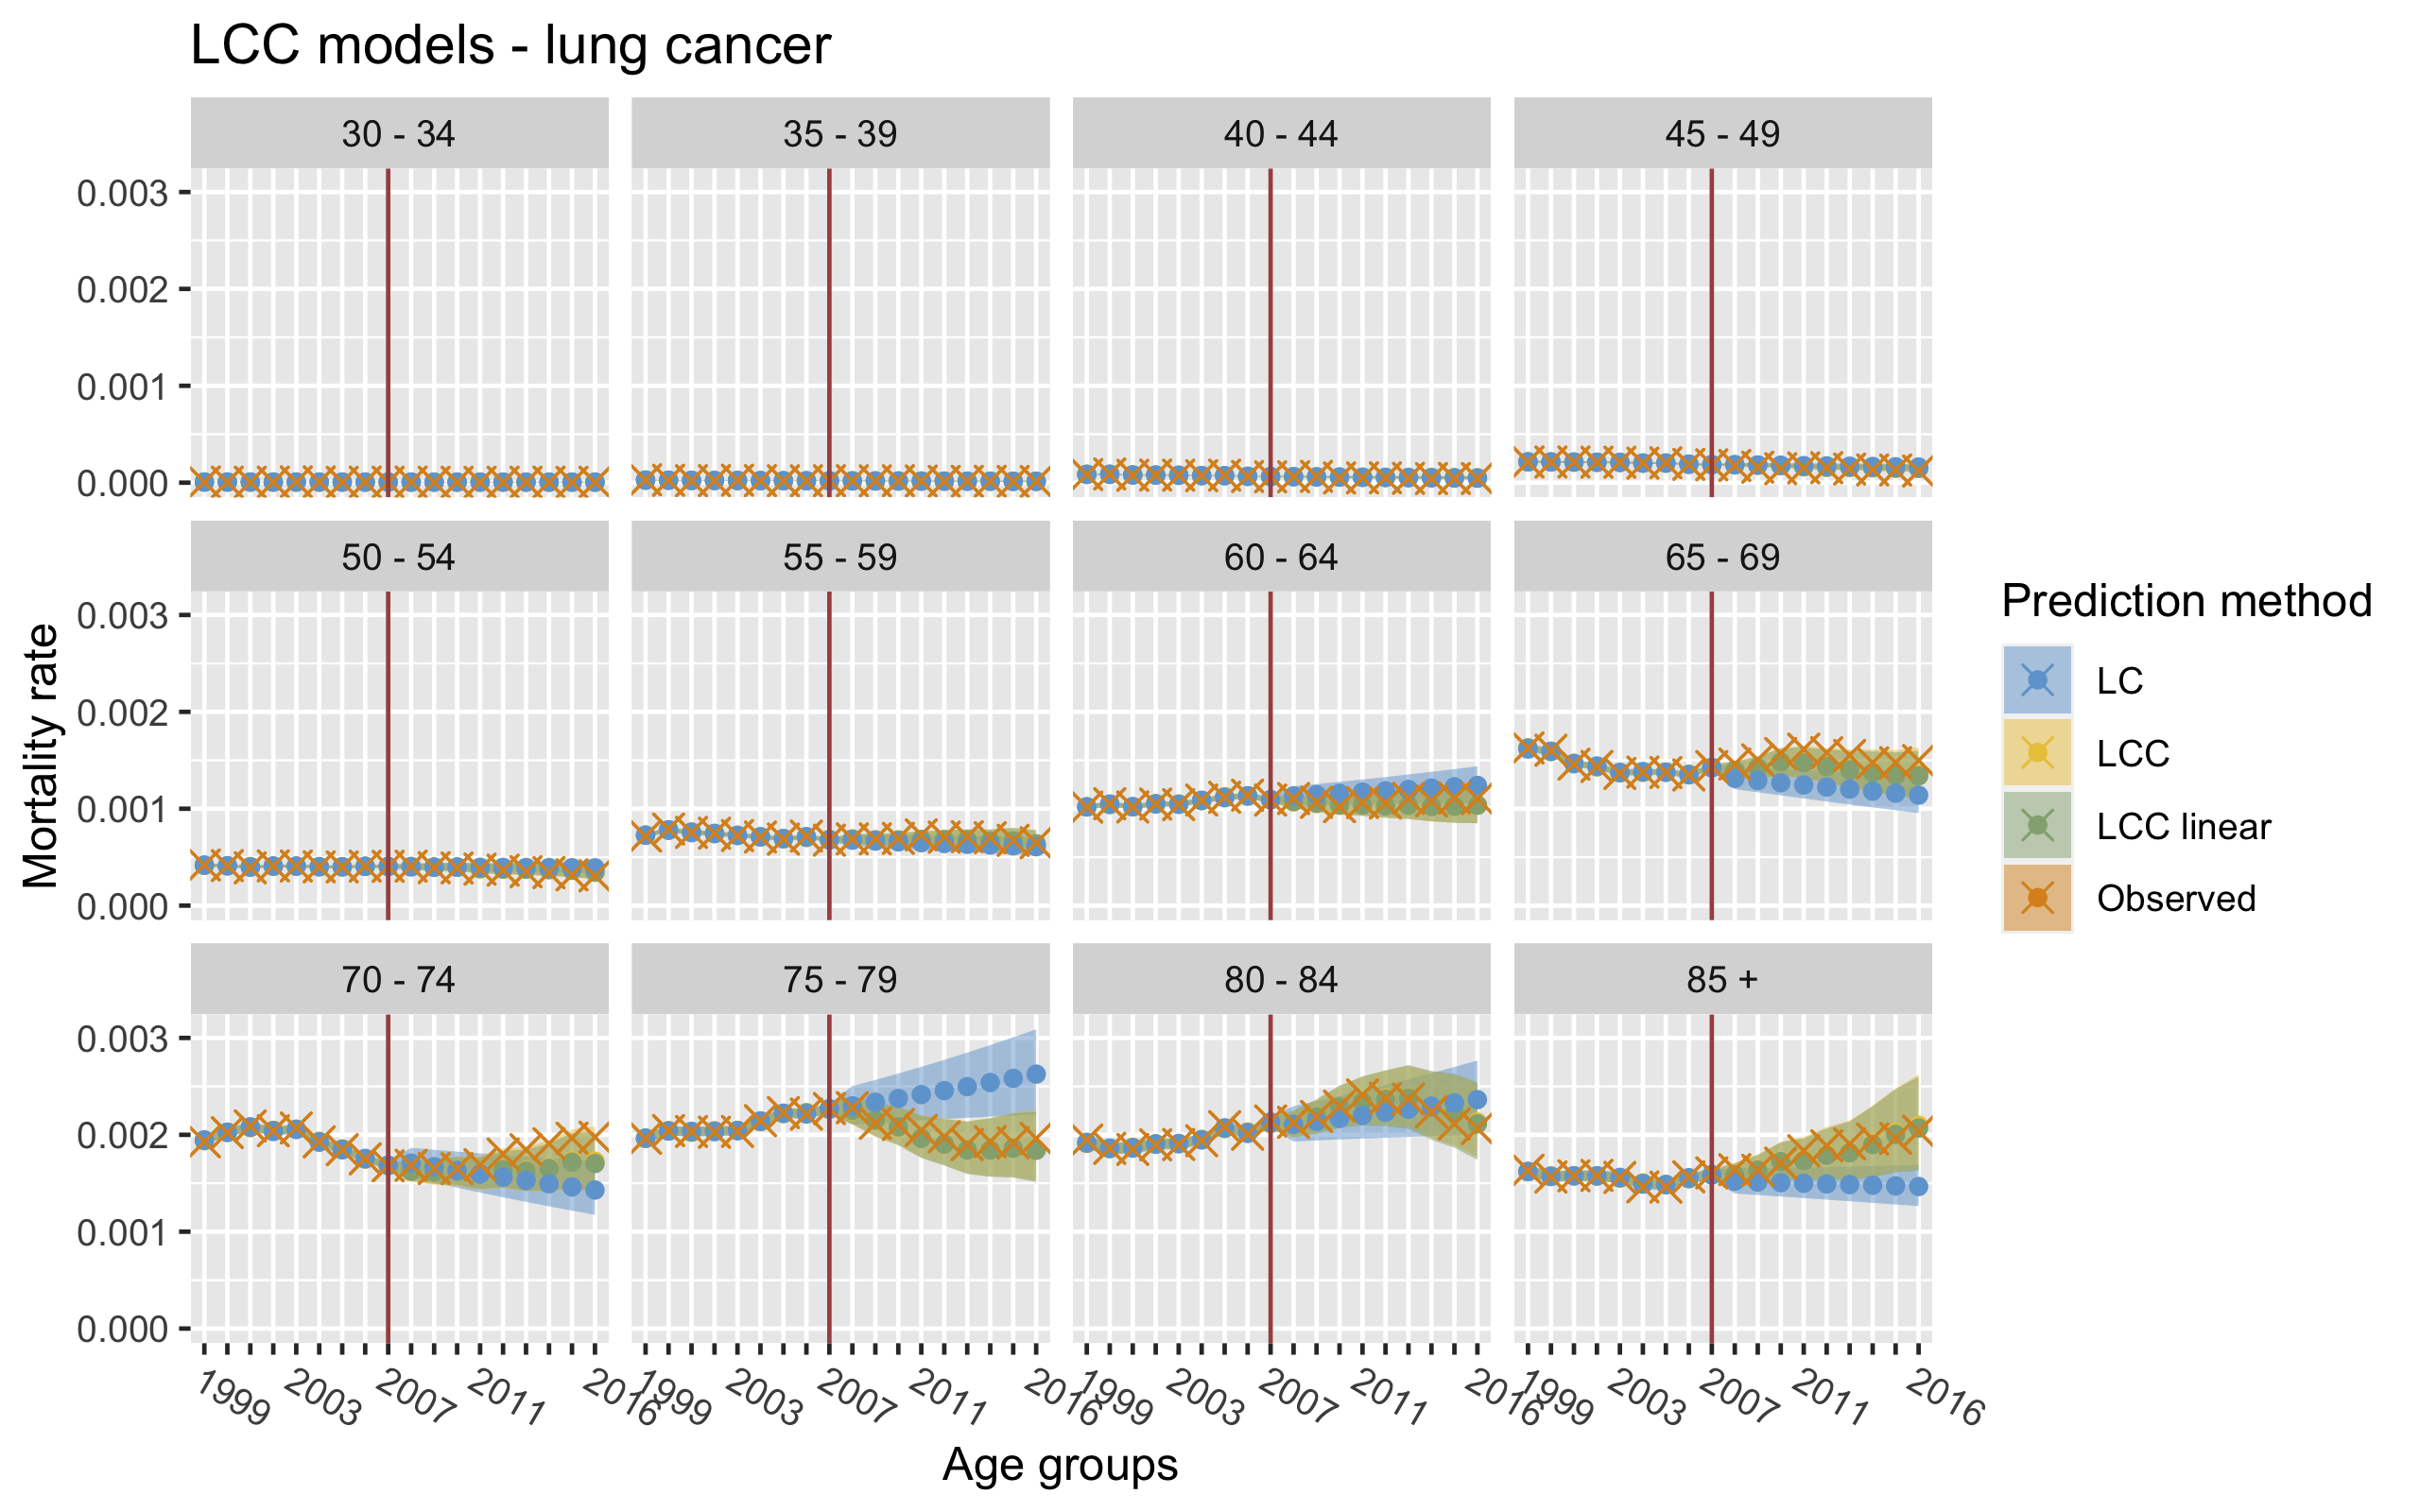
\includegraphics[width=\linewidth]{real-data/real-data-univariate/Figures/univariate-LCC-by-period-lung.png}
        \caption{The prediction results plotted for each age group that are 30 years and older, with the calendar years along the horizontal axis. The red line marks the beginning of the predicted periods. }
        \label{fig:uv-LCC-lung-bottom}
    \end{subfigure}
    \caption{The mean values and the 95\% confidence bounds of the predicted expected lung cancer mortality rates produced by inference with three Lee-Carter types of models on data of German lung cancer (circles), together with the corresponding observed mortality rates $Y_{x,y}^{\text{lung}}$ (crosses).
    }
    \label{fig:uv-LCC-lung}
\end{figure}

\begin{figure}[h!]
    \centering
    \begin{subfigure}[b]{.75\linewidth}
        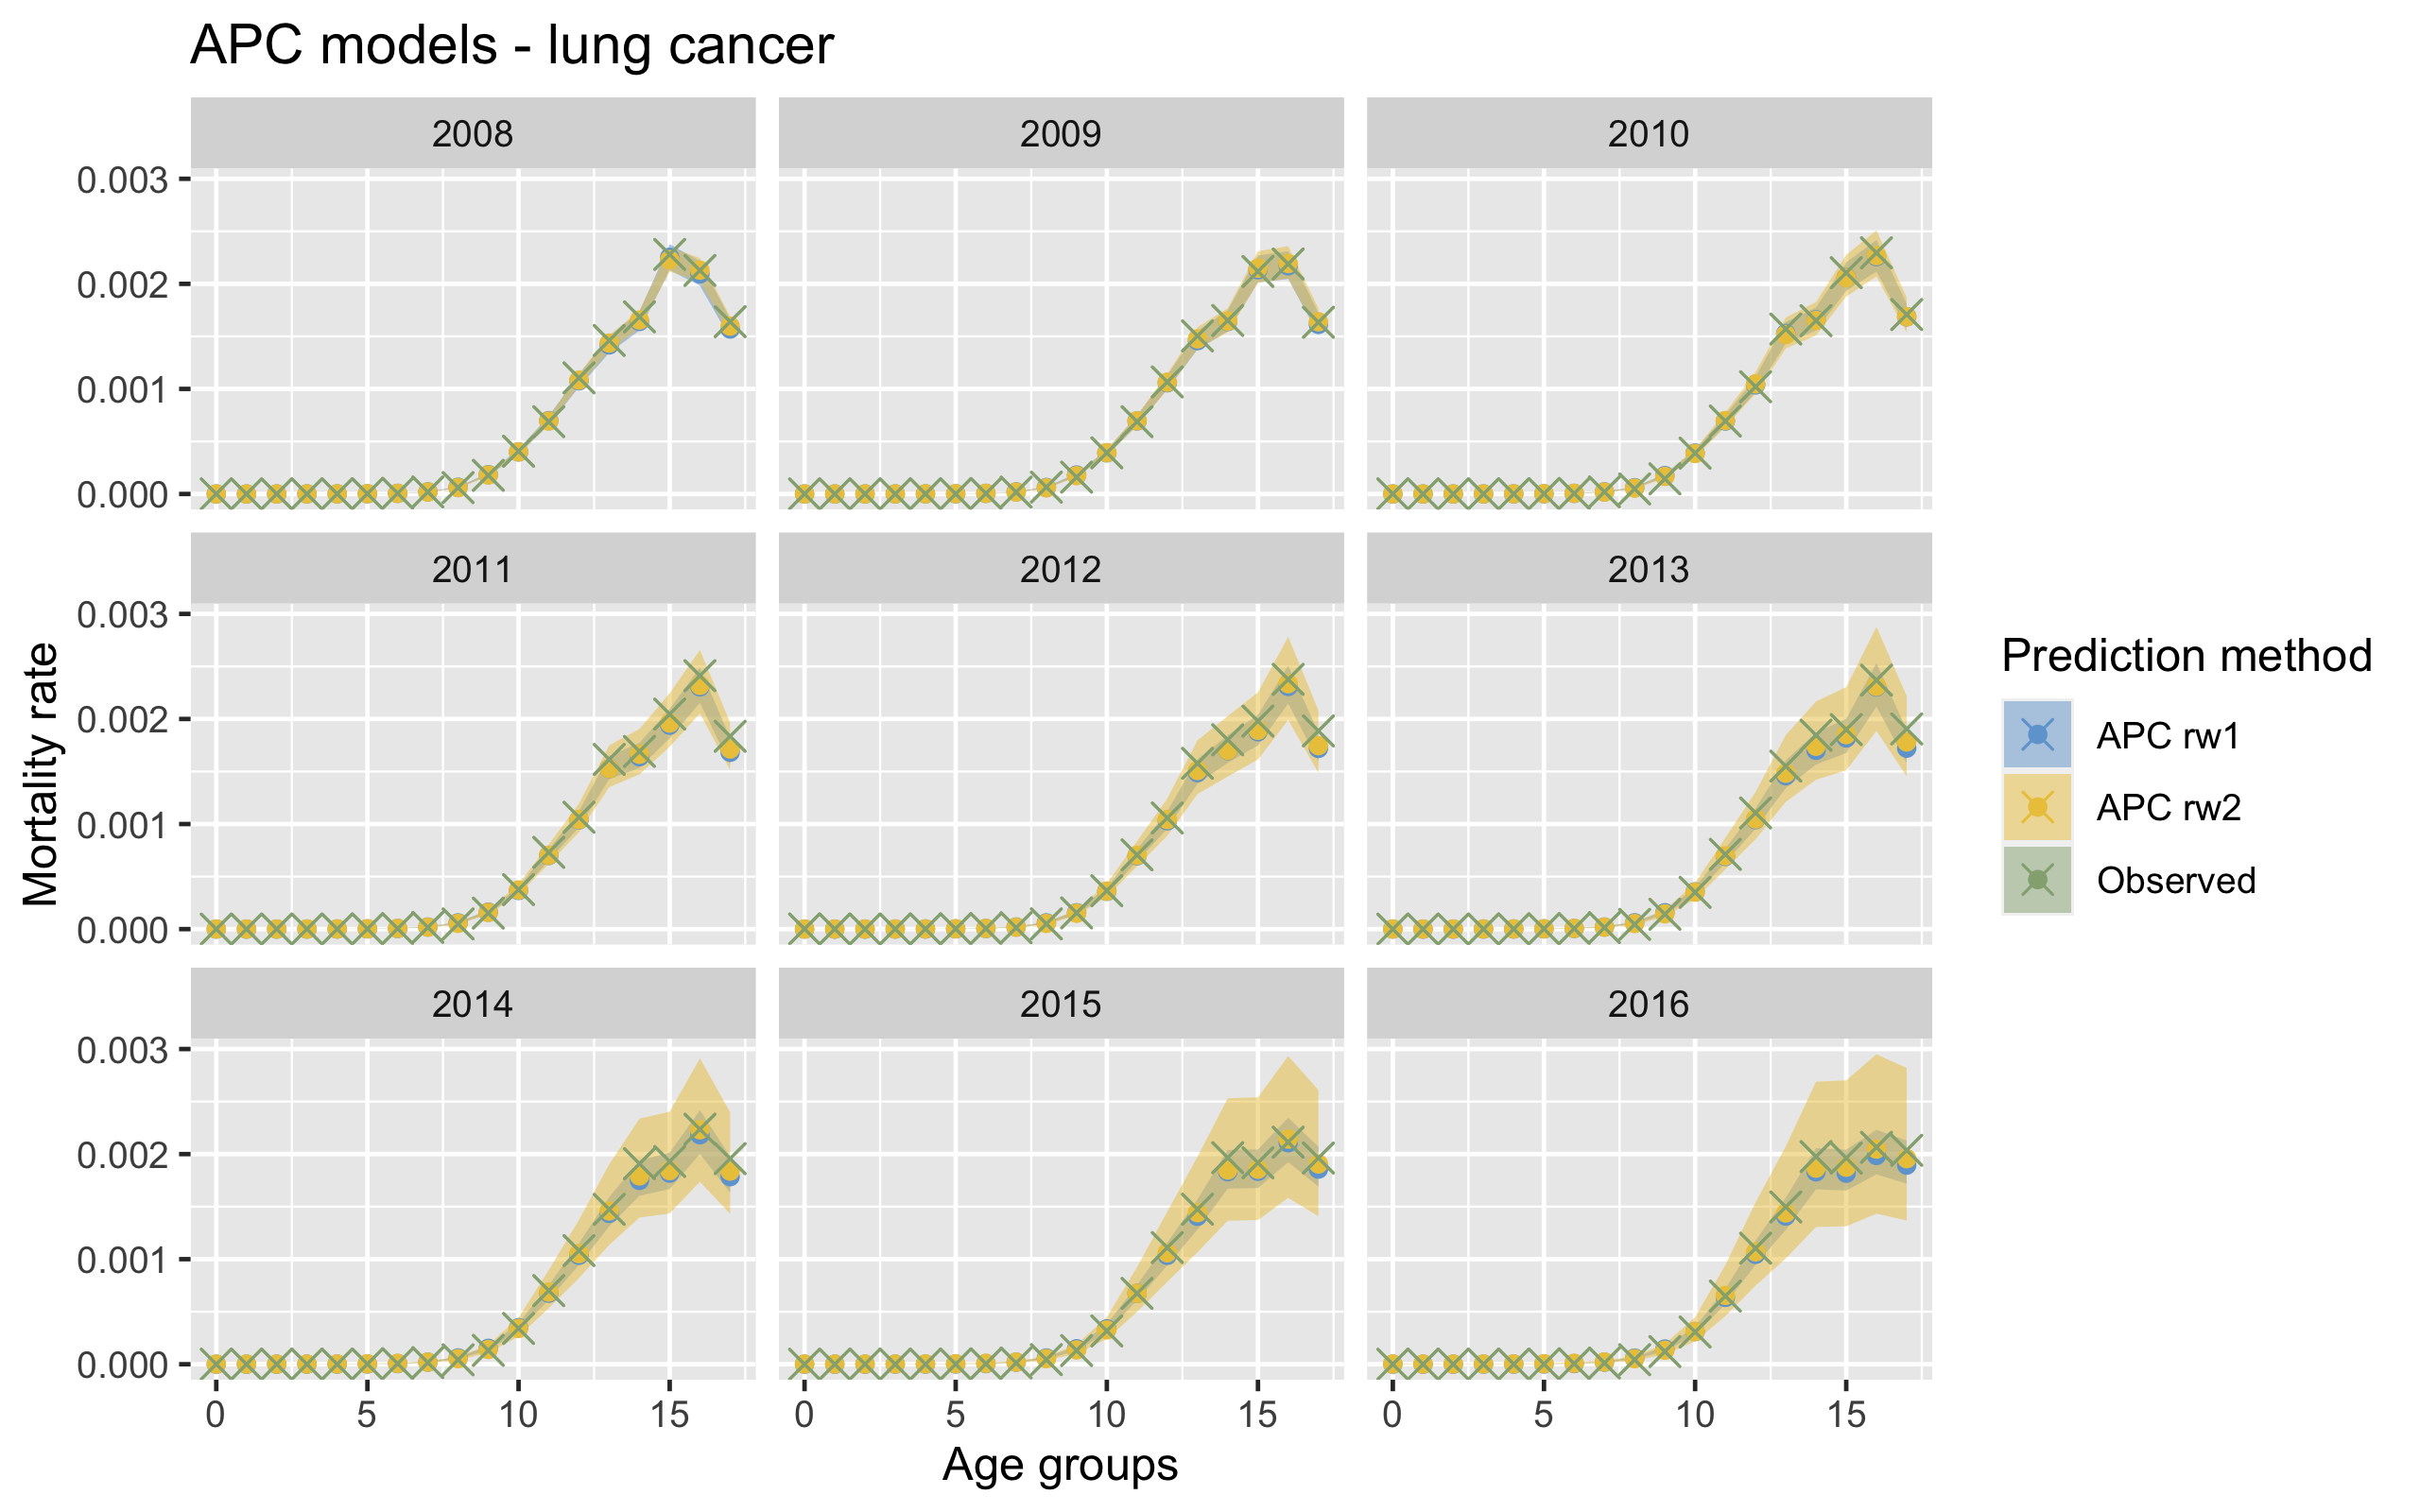
\includegraphics[width=\linewidth]{real-data/real-data-univariate/Figures/univariate-APC-by-age-lung.png}
        \label{fig:uv-APC-lung}
    \end{subfigure}
    
    \begin{subfigure}[b]{.75\linewidth}
        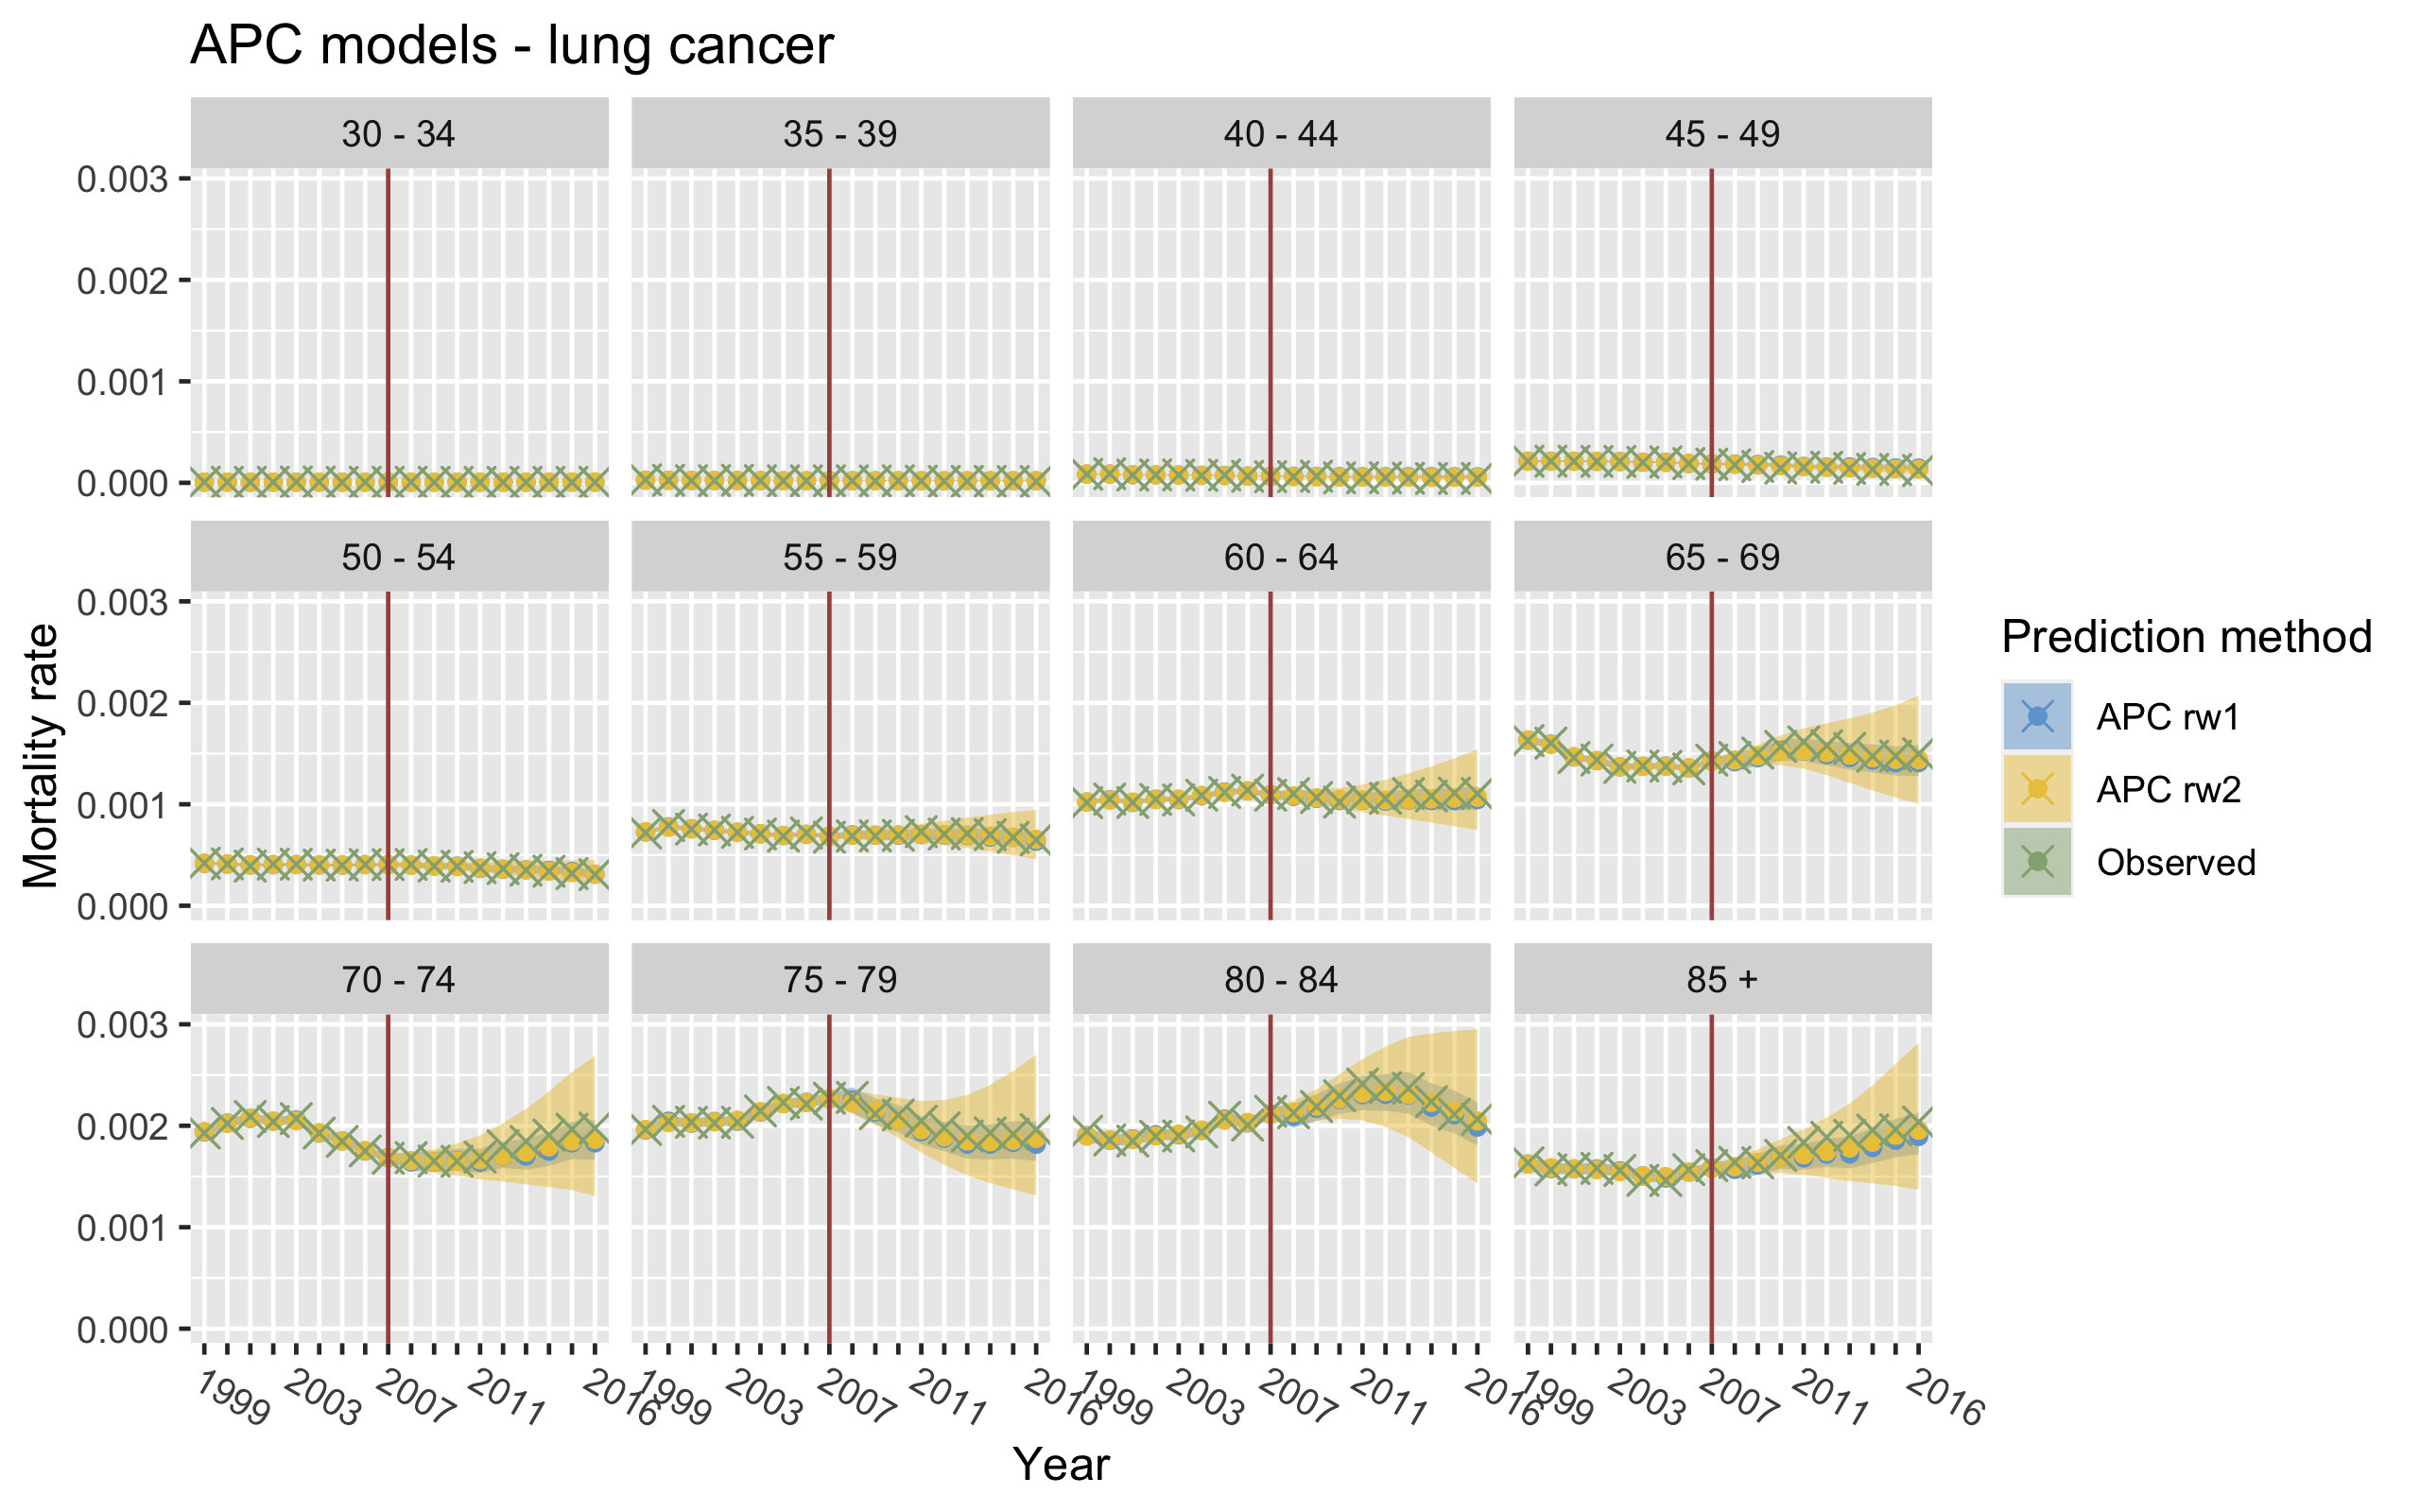
\includegraphics[width=\linewidth]{real-data/real-data-univariate/Figures/univariate-APC-by-period-lung.png}
        \label{fig:uv-APC-lung-bottom}
    \end{subfigure}
    \caption{The mean values and the 95\% confidence bounds of the predicted expected lung cancer mortality rates produced by inference with the APC1- and the APC2-model on data of German lung cancer (circles), together with the corresponding observed mortality rates $Y_{x,y}^{\text{lung}}$ (crosses). The layout of the plots is similar to that of Figure \ref{fig:uv-LCC-lung}}
    \label{fig:uv-APC-lung}
\end{figure}

\begin{table}[h!]
    \begin{center}
        \begin{tabular}{l |c c c }
            Model & MSE &   MDSS & Contained 95\%-interval\\
            \hline
            APC1    & 3.896e-9 & -19.27    & 0.7778 \\
            APC2    & 2.174e-9 & -19.88    & 0.8889 \\
            LC      & 5.144e-8 & -16.02    & 0.6204 \\
            LCC     & 4.746e-9 & -20.12    & 0.9907 \\
            LCC-linear      & 5.238e-9 & -20.01    & 0.9722 \\
        \end{tabular}
        \caption{Score statistics for different models applied to the lung cancer data, calculated for predictions where $x > 5$.}\label{tbl:uv-lung-5}
    \end{center}
\end{table}

\newpar Figures \ref{fig:uv-LCC-lung} and \ref{fig:uv-APC-lung} display the prediction results for lung cancer mortality, using the Lee-Carter and the APC methods, respectively. We present the predictions for each predicted year, with age groups along the x-axis (the left-most image in the figures) and for each age group, with all years along the x-axis (right-most image in the figures). For the images where results are displayed by age groups, we only show the results for ages above 30. This is simply because the real and predicted mortality rates are very close to zero for younger ages, so these results are not very interesting. The red line marks the division between fitted and predicted mortality rates. 

\newpar The score statistics for these results are displayed in Table \ref{tbl:uv-lung-5}. For younger ages, below ca. 30 years old, the mortality rates for both lung- and stomach cancer are very low, almost at zero. All methods gives a prediction very close to zero with narrow prediction intervals for these ages, and we are more interested in evaluating the prediction methods for mortality rates that are significantly greater than zero. Therefore, we omit the prediction values for $x \leq 5$, corresponding to ages less than 30, when calculating the score statistics. We then get a better impression of the quality of the prediction of non-zero mortality rates. 

Table \ref{tbl:uv-stomach-5} show the same results for predictions of stomach cancer mortality, and the corresponding plotted results are displayed in Figures \ref{fig:uv-LCC-stomach} and \ref{fig:uv-APC-stomach} in the appendix. 
\newpar From Figures \ref{fig:uv-LCC-lung} and \ref{fig:uv-LCC-stomach}, we observe that for both lung and stomach cancer, the LCC and LCC-linear models produce significantly better predictions than the LC-model. This difference is especially apparent for the older age groups. The LCC- and the LCC-linear models seem, from the plotted results, to give very similar, and quite good, predictions. These observations are confirmed by the score statistics in Tables \ref{tbl:uv-lung-5} and \ref{tbl:uv-stomach-5}. The MDSS for the LC-model is clearly higher than the MDSS for the LCC and the LCC-linear models, which is a clear indication that the LC-model performs worse than the others. The LCC and the LCC-linear models have very similar score statistics. The MDSS for the LCC model is slightly lower than the MDSS for the LCC-linear model, both for lung and stomach cancer, indicating that the former gives better predictions. Since this was our original proposed model, and we do not seem to gain performance in prediction by omitting the non-linear period term $\kappa_t$, we keep this model in our following investigation. Still, we underline that it seems like most of the period-related variability in the mortality rates can be explained by a linear trend.

\begin{table}
    \begin{center}
        \begin{tabular}{l |c c c }
            Model & MSE &   MDSS & Contained 95\%-interval\\
            \hline
            APC1     & 1.969e-9 & -19.12    & 0.7963 \\
            APC2     & 5.840e-9 & -19.52    & 0.9167 \\
            LC      & 6.851e-8 & -15.50    & 0.5926 \\
            LCC     & 1.112e-8 & -19.46    & 0.9352 \\
            LCC-linear      & 1.141e-8 & -19.39    & 0.8889
        \end{tabular}
        \caption{Score statistics for different models applied to the stomach cancer data, calculated for predictions where $x > 5$.}\label{tbl:uv-stomach-5}
    \end{center}
\end{table}

\newpar For the two APC models, APC1 and APC2, it is less clear which model perform the best. Figures \ref{fig:uv-APC-lung} and \ref{fig:uv-APC-stomach} display the results from using the APC models to predict lung and stomach cancer mortality. Firstly, we note that both the APC1 and APC2-models seem to predict the mortality rates well, both for lung and stomach cancer. We observe that for both cancer types, the APC2-model produces predictions with wider prediction intervals than the APC1-model does. We also observe that the prediction intervals from the APC2-model is widening with more recent years (the predictions get less sharp further into the future). This tendency is not as clear for the APC1-model. For lung cancer mortality, we observe from Figure \ref{fig:uv-APC-lung} that the APC2 predictions might be slightly more accurate than the APC1 predictions. We especially see this tendency for older age groups. From Tables \ref{tbl:uv-lung-5} and \ref{tbl:uv-stomach-5} we observe that the APC2 model has a slightly lower MDSS for both cancer types.
However, we note that it seems like what age we set as the cut-off when calculating the MDSS influence which of the APC1 and APC2-models get the lowest MDSS. The score statistics calculated using only ages where $x > 8$ for the lung cancer prediction are displayed in Table \ref{tbl:uv-lung-8}, and corresponding score statistics for the stomach cancer predictions are included in Table \ref{tbl:uv-stomach-8} in the appendix. We observe that for these predictions, the APC1-model has a slightly lower MDSS than the APC2-model. We also see that the percentage of observations contained in the 95\% prediction intervals are higher for the APC2-model, while the MSE is lower for the APC1 compared to the APC2-model. This is in line with the wide prediction intervals for the APC2-model that we observe from the plotted results. We interpret this as an indication that for stomach and lung cancer, the APC1-model is better suited to model mortality rates for older age groups. Still, since we originally decided to calculate the score statistics using all ages from 30 years and older ($x > 5$), we will base our following investigation on these scores and consider only the APC2-model from this point on. 

\begin{table}[h!]
    \begin{center}
        \begin{tabular}{l |c c c }
            Model & MSE &   MDSS & Contained 95\%-interval\\
            \hline
            APC1    & 5.174e-9 & -18.74    & 0.9136 \\
            APC2    & 2.889e-9 & -18.64    & 0.9753 \\
            LC         & 6.859e-8 & -12.95    & 0.4938 \\
            LCC        & 6.322e-9 & -18.49    & 0.9877 \\
            LCC-linear & 6.977e-9 & -18.40    & 0.9753 \\
        \end{tabular}
        \caption{Score statistics for different models applied to the lung cancer data, calculated for predictions where $x > 8$.}\label{tbl:uv-lung-8}
    \end{center}
\end{table}

\begin{figure}[h!]
    \centering
    \begin{subfigure}[b]{.75\linewidth}
        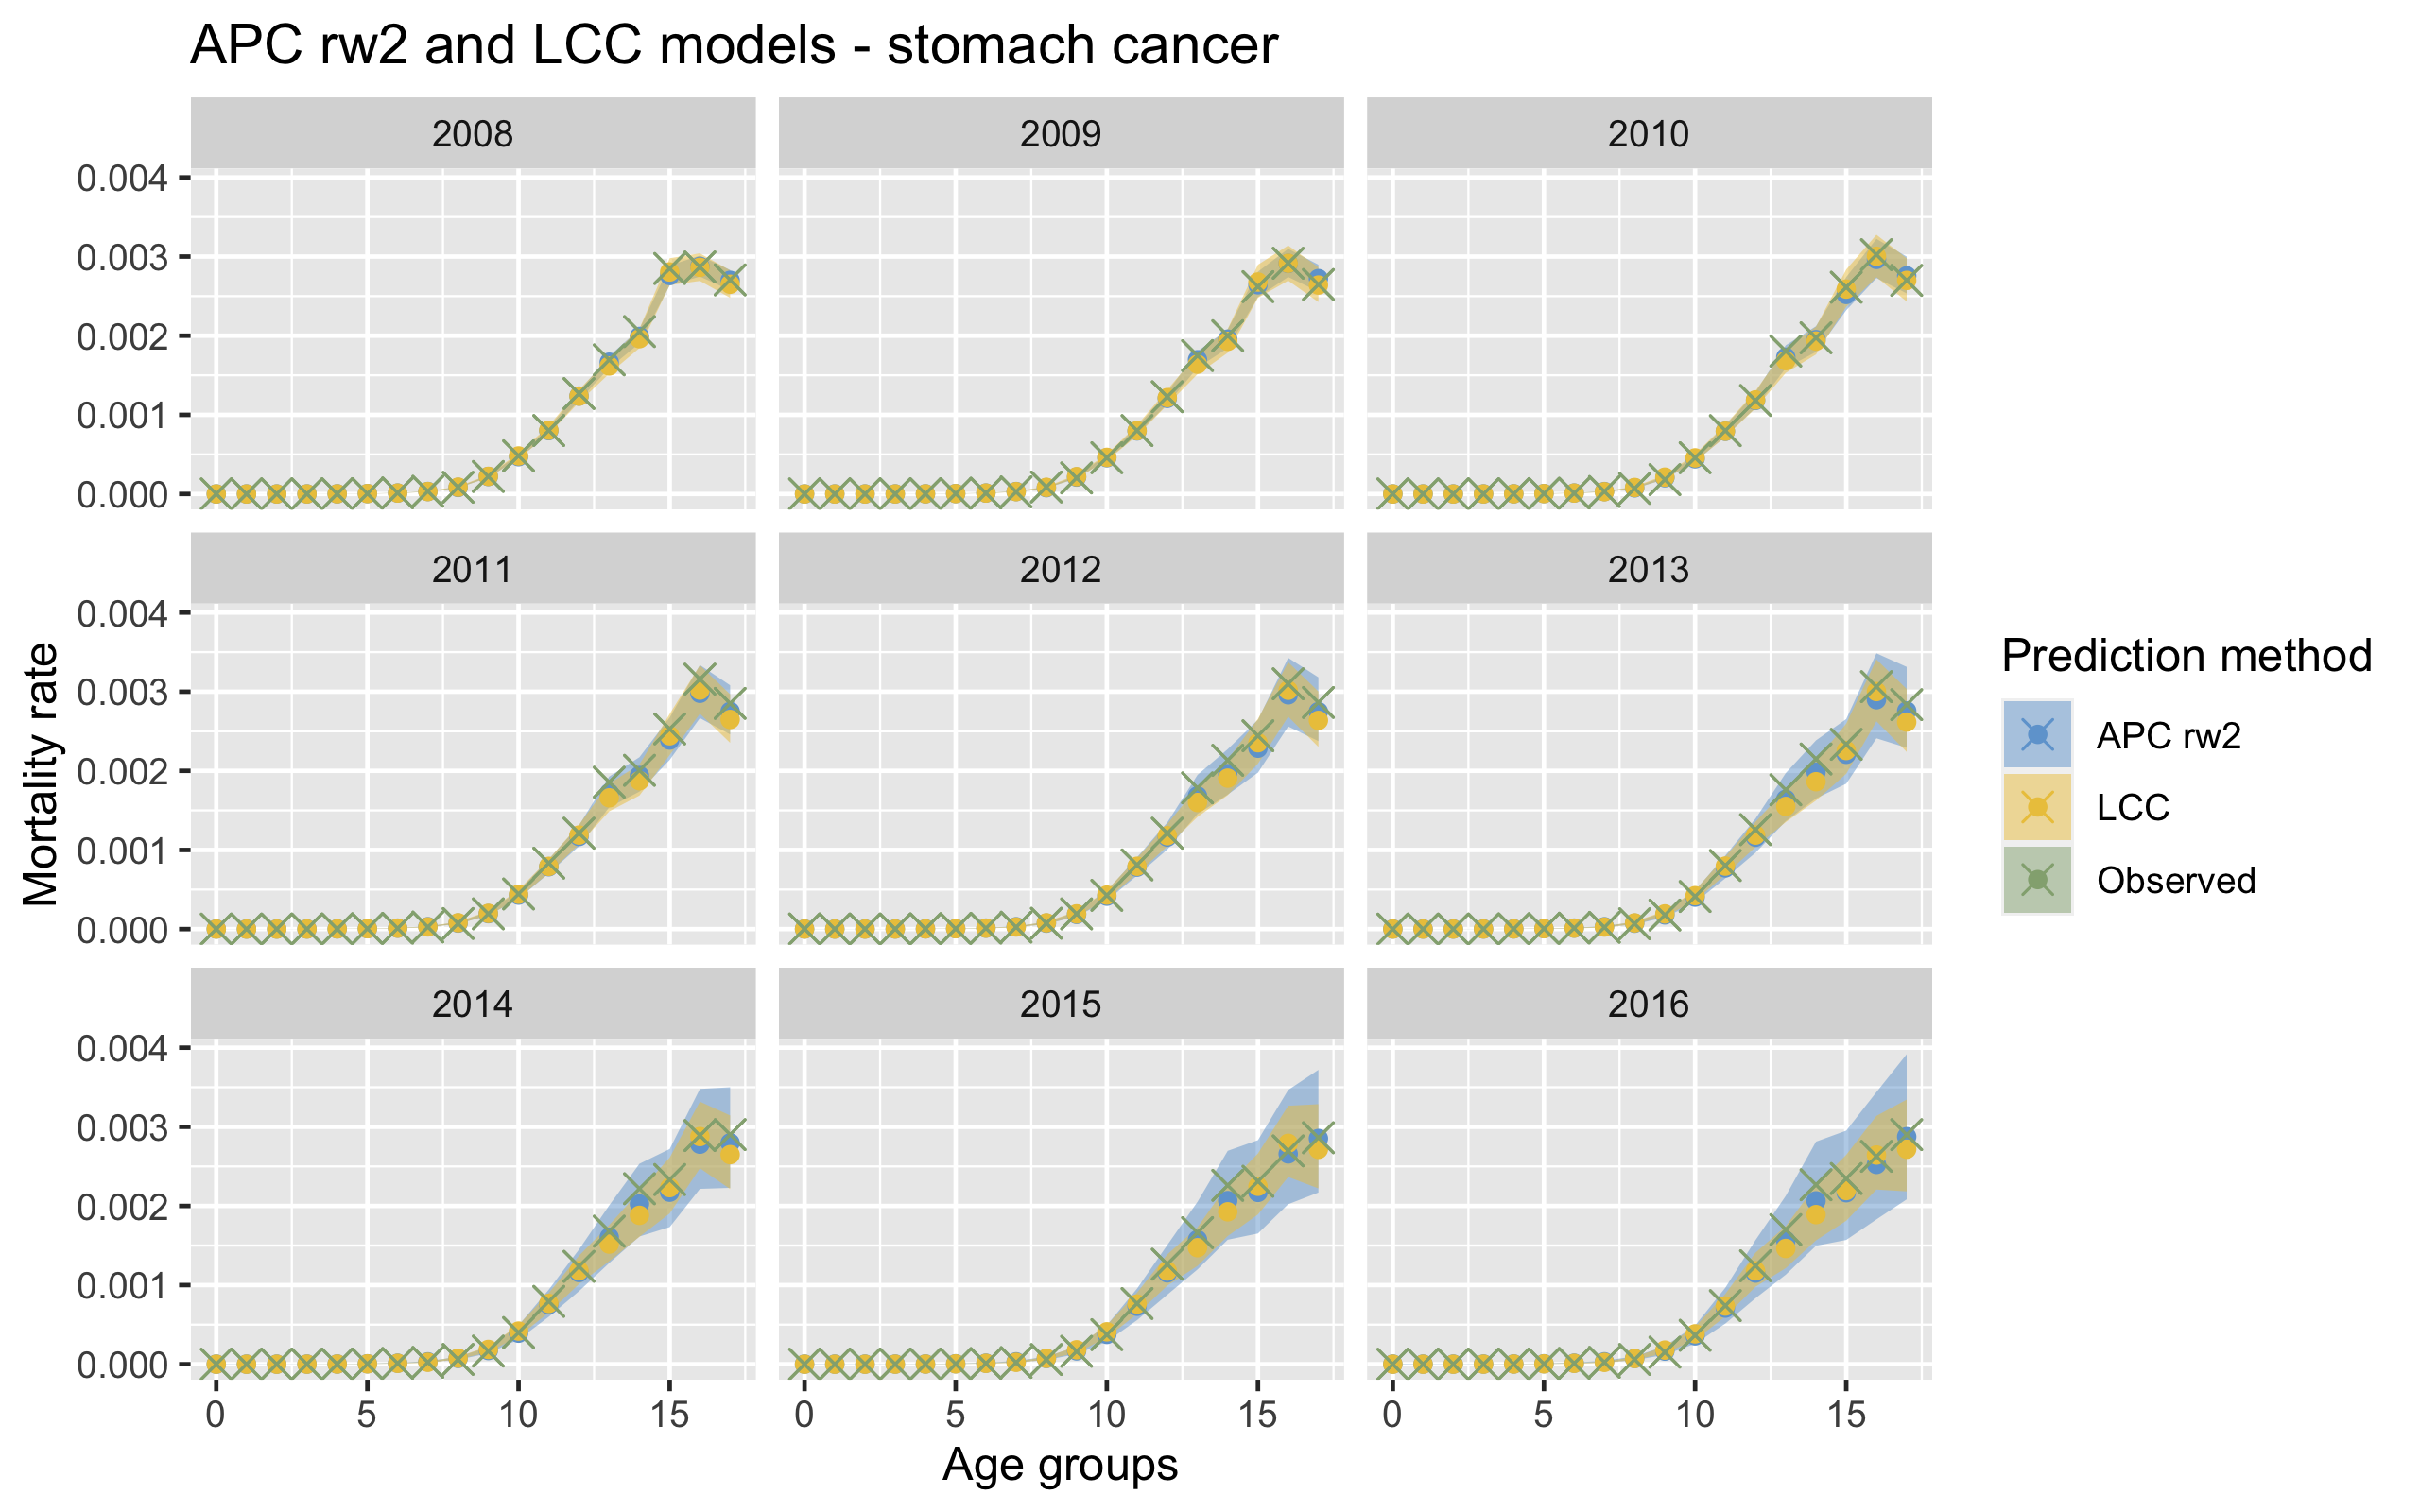
\includegraphics[width=\linewidth]{real-data/real-data-univariate/Figures/univariate-comparison-by-age-lung.png}
        \label{fig:uv-comparison-lung-top}
    \end{subfigure}
    
    \begin{subfigure}[b]{.75\linewidth}
        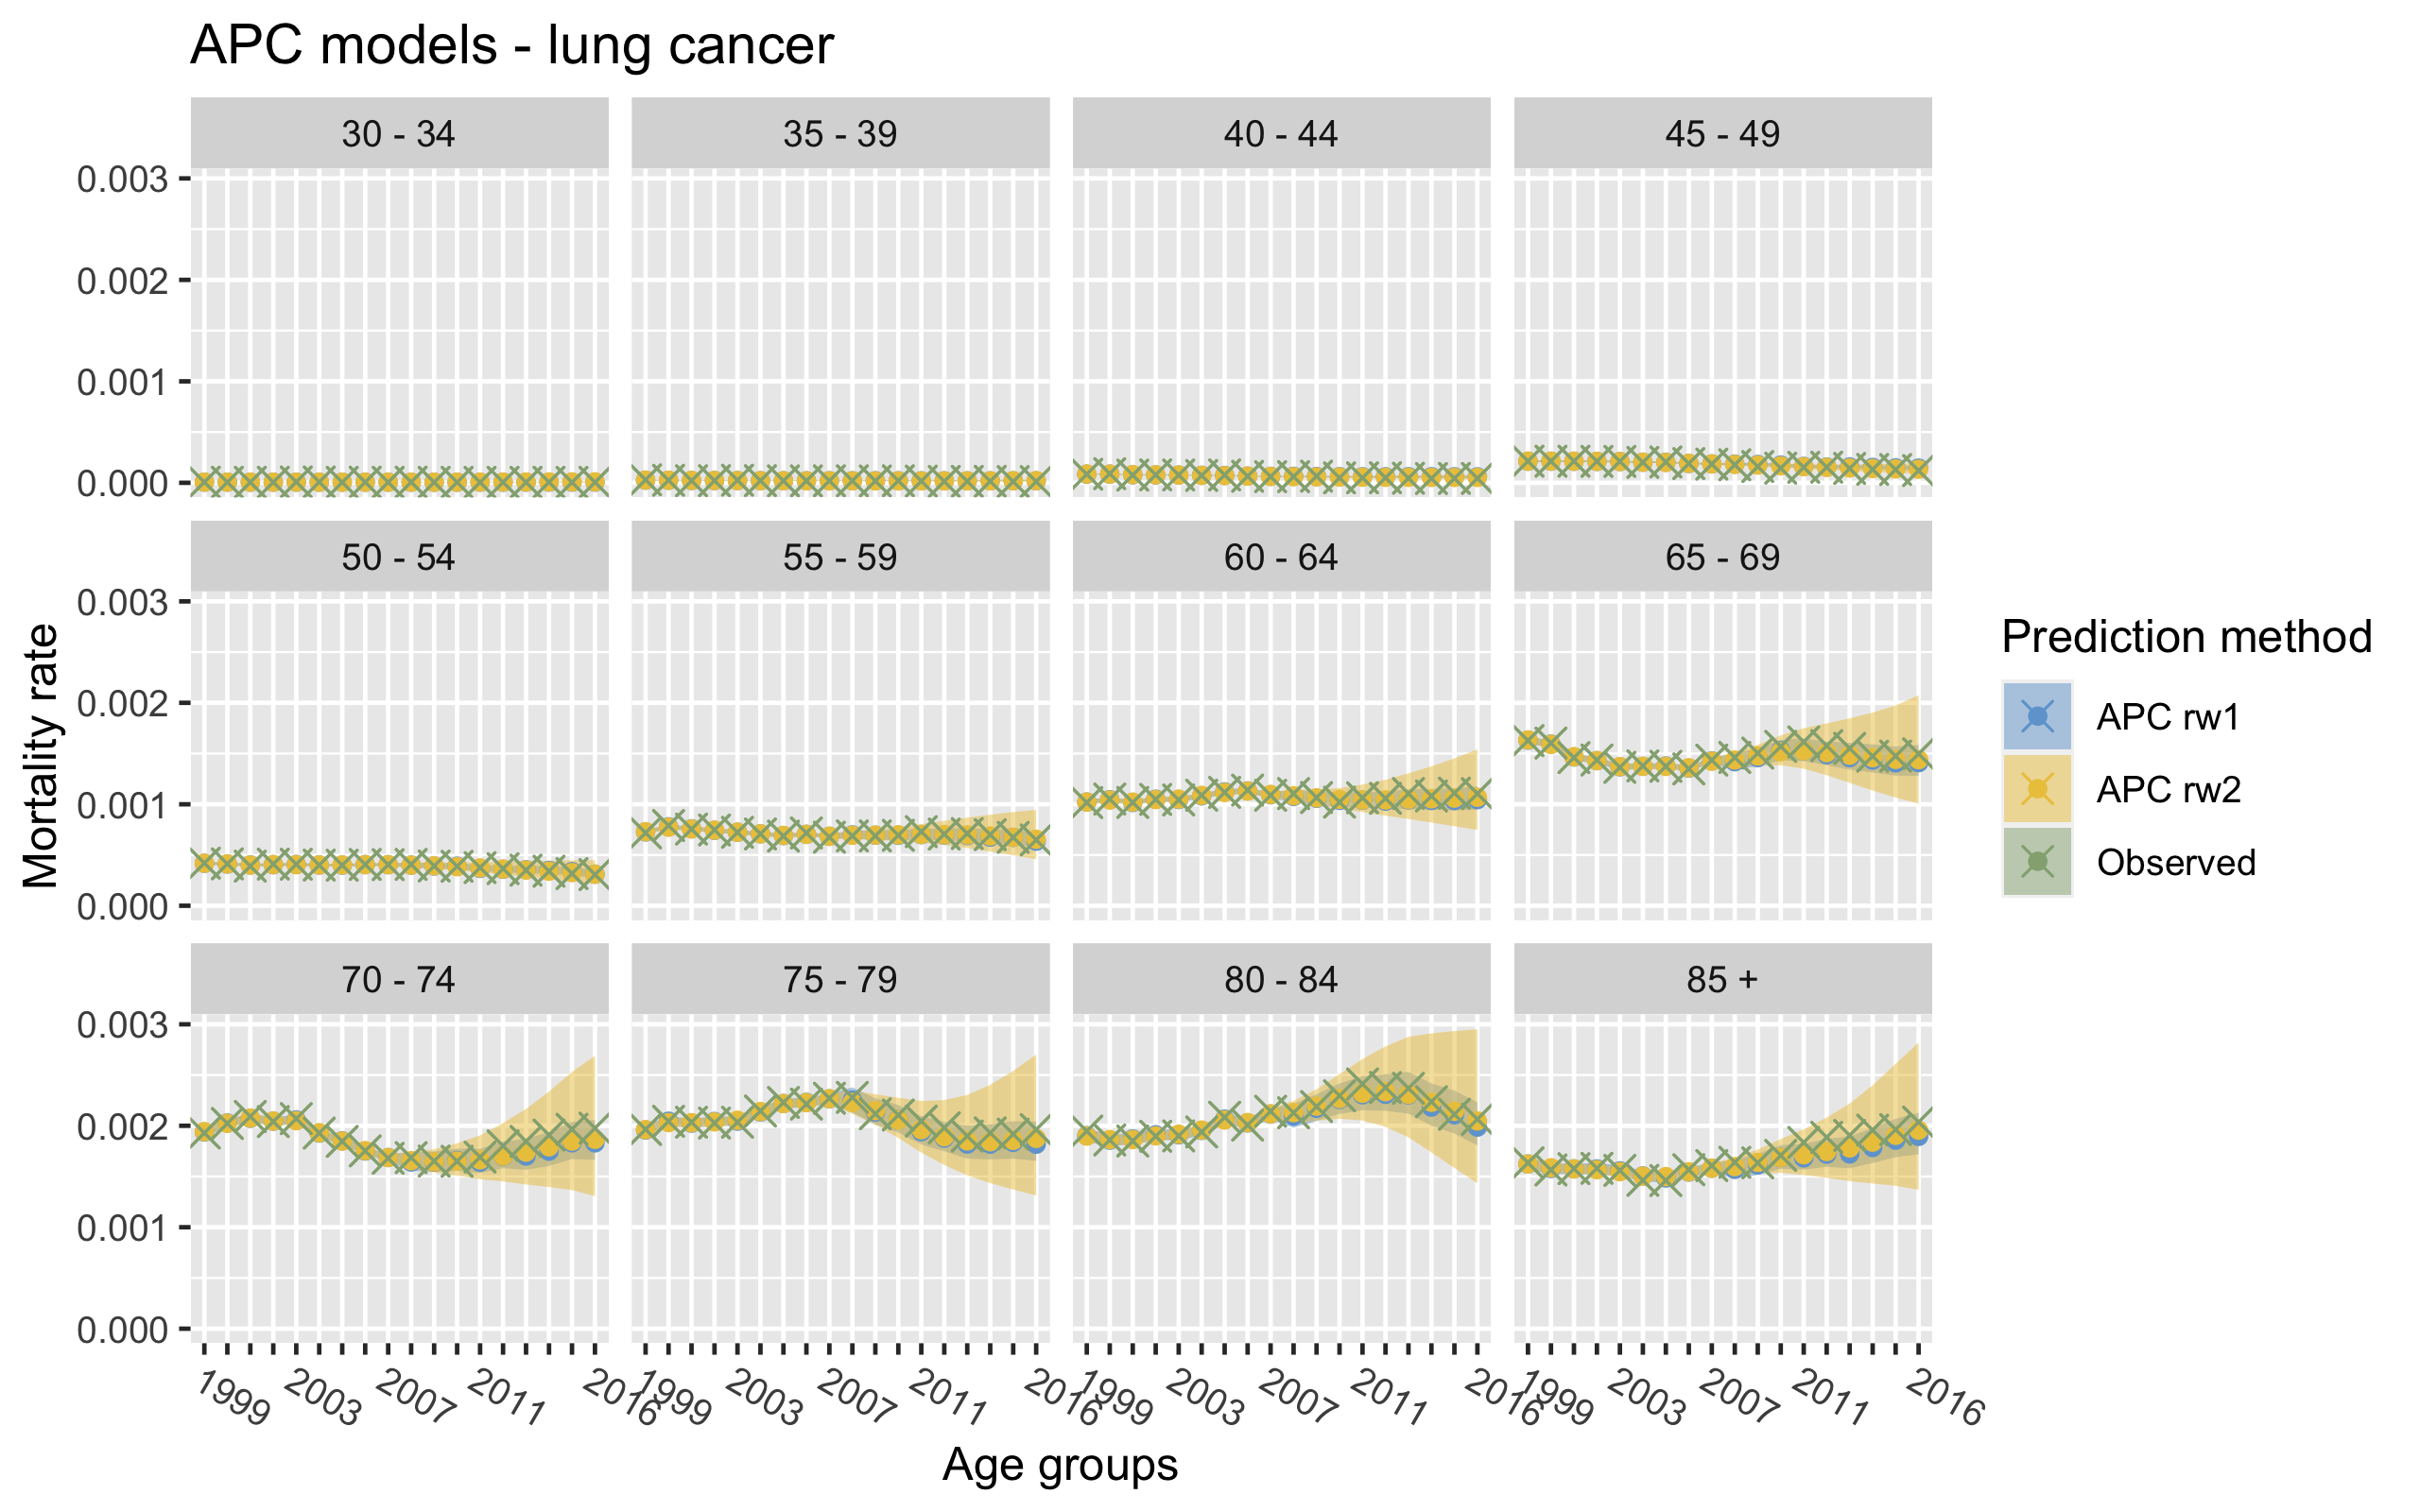
\includegraphics[width=\linewidth]{real-data/real-data-univariate/Figures/univariate-comparison-by-period-lung.png}
        \label{fig:uv-comparison-lung-bottom}
    \end{subfigure}
    \caption{The mean values and the 95\% confidence bounds of the predicted expected lung cancer mortality rates produced by inference with the APC2- and the LCC-model on data of German lung cancer (circles), together with the corresponding observed mortality rates $Y_{x,y}^{\text{lung}}$ (crosses). The layout of the plots is similar to that of Figure \ref{fig:uv-LCC-lung}}
    \label{fig:uv-comparison-lung}
\end{figure}

\begin{figure}[h!]
    \centering
    \begin{subfigure}[b]{.6\linewidth}
        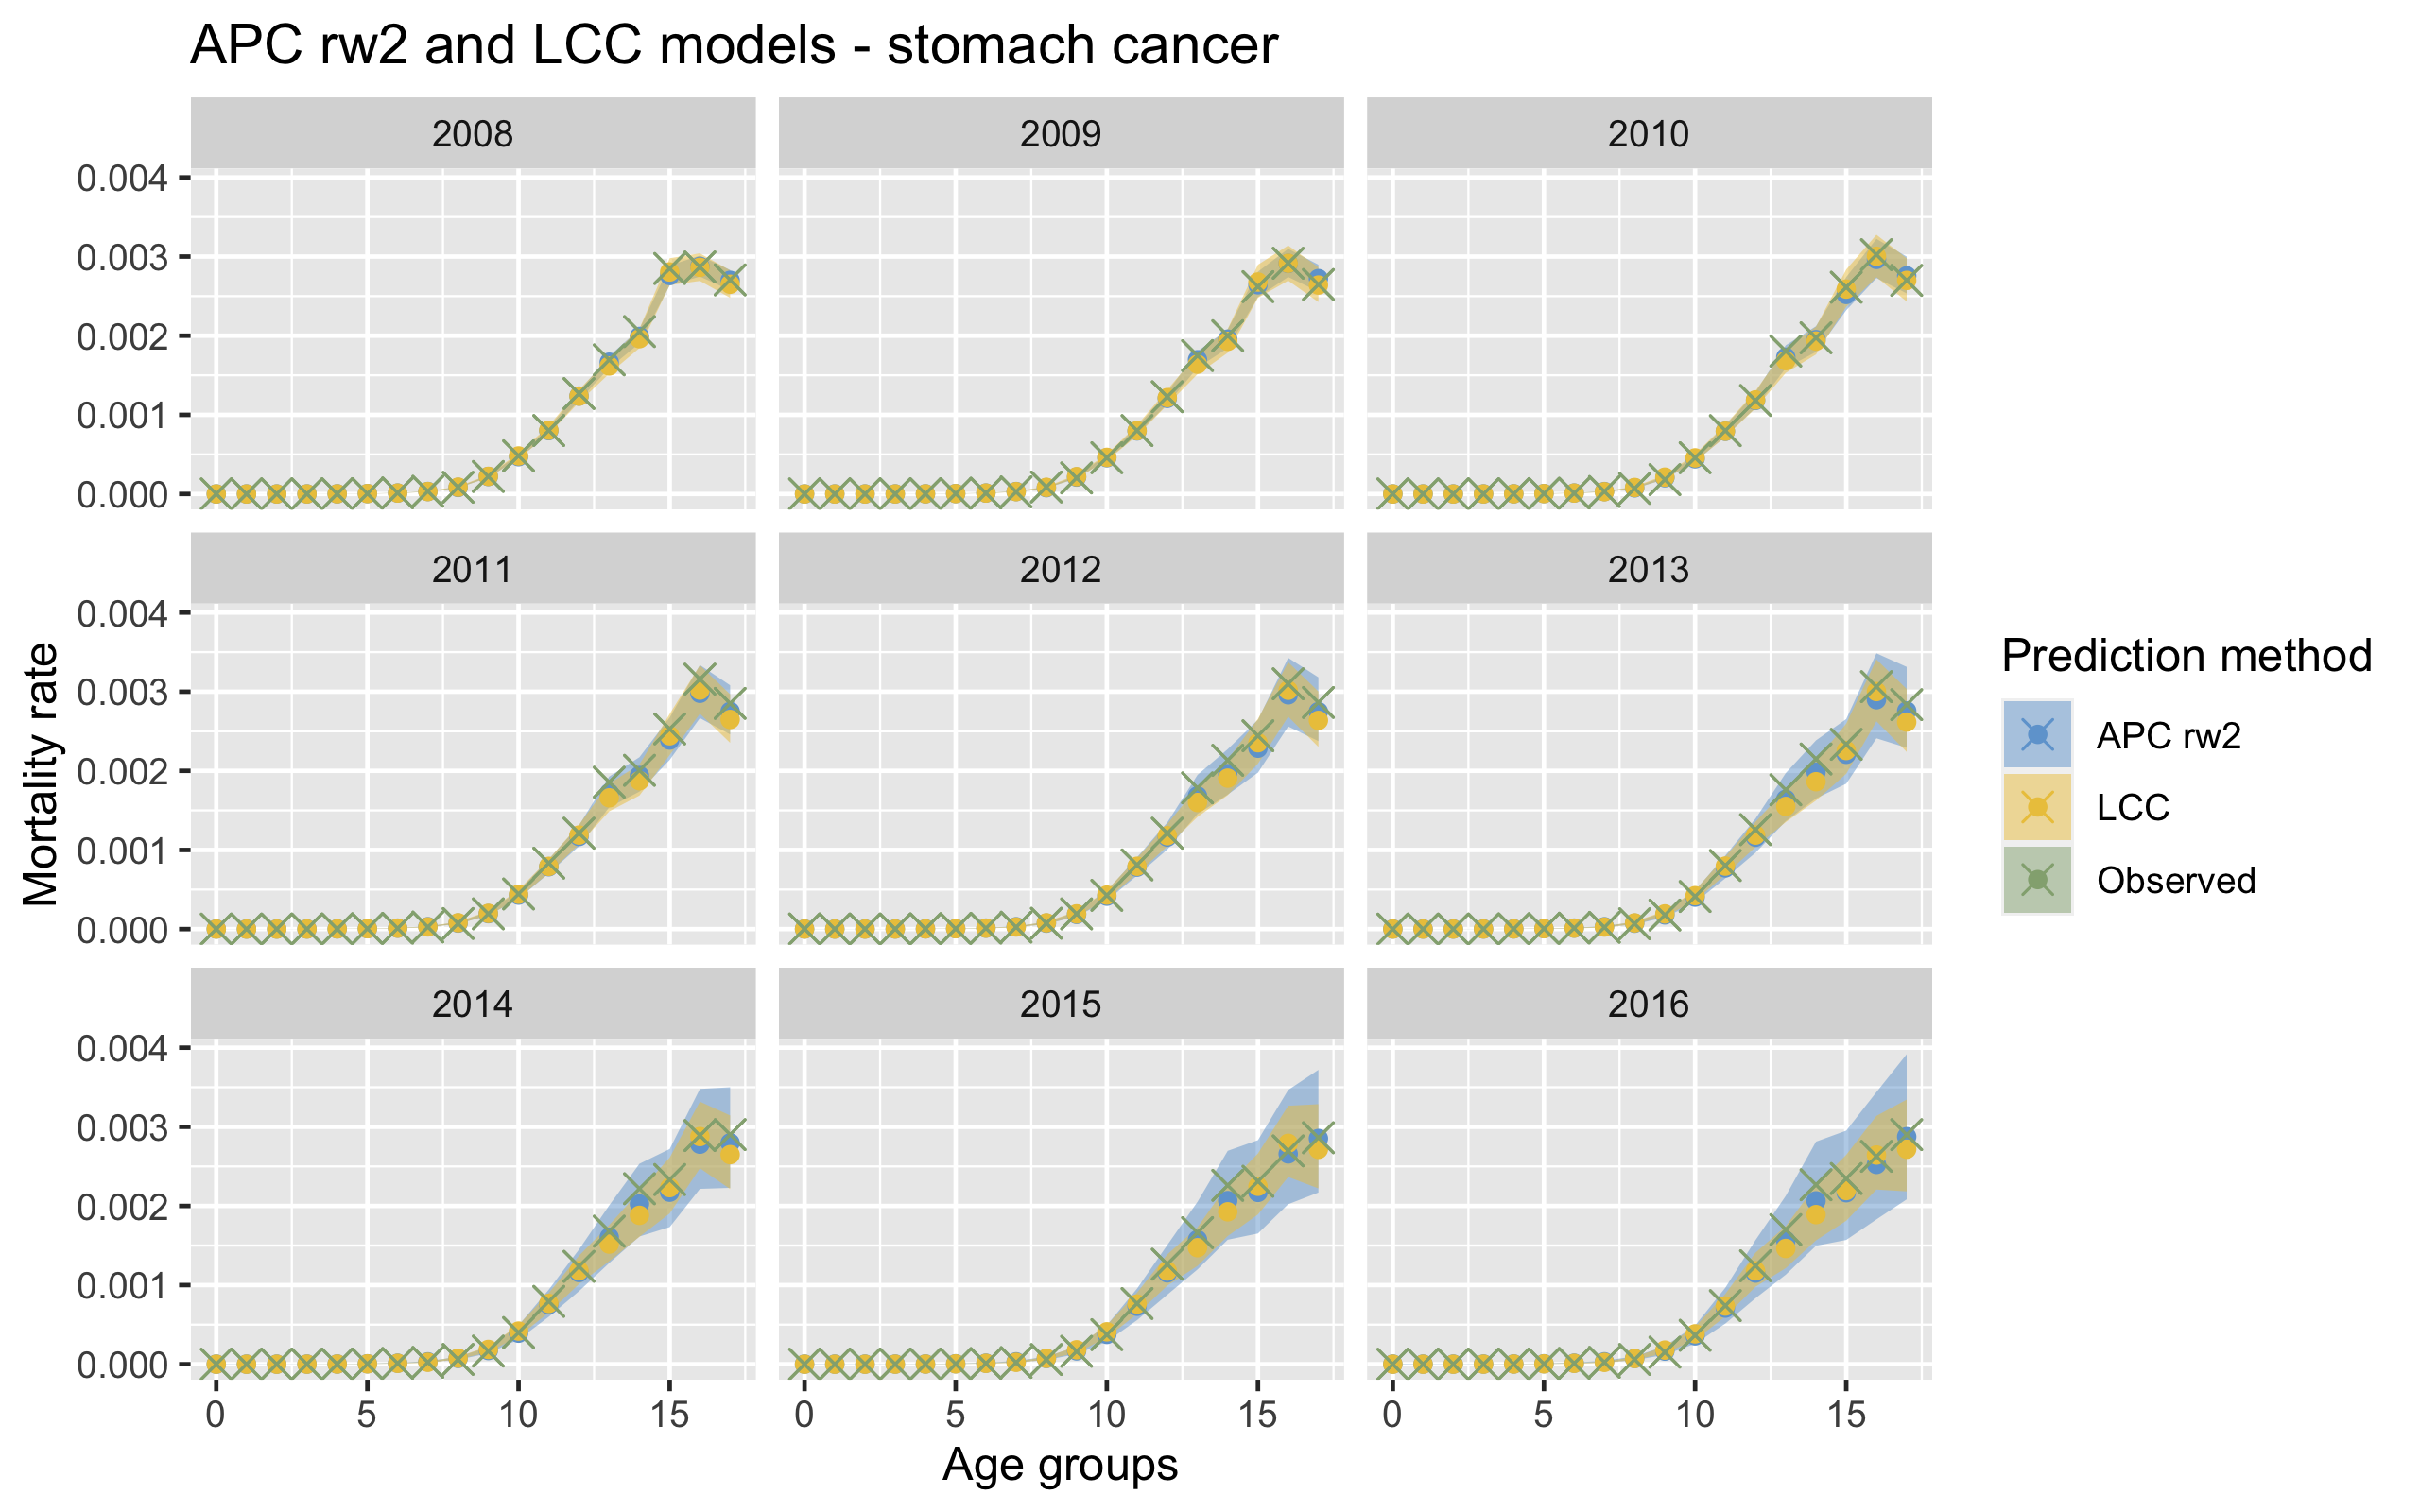
\includegraphics[width=\linewidth]{real-data/real-data-univariate/Figures/univariate-comparison-by-age-stomach.png}
        \label{fig:uv-comparison-stomach-top}
    \end{subfigure}
    
    \begin{subfigure}[b]{.6\linewidth}
        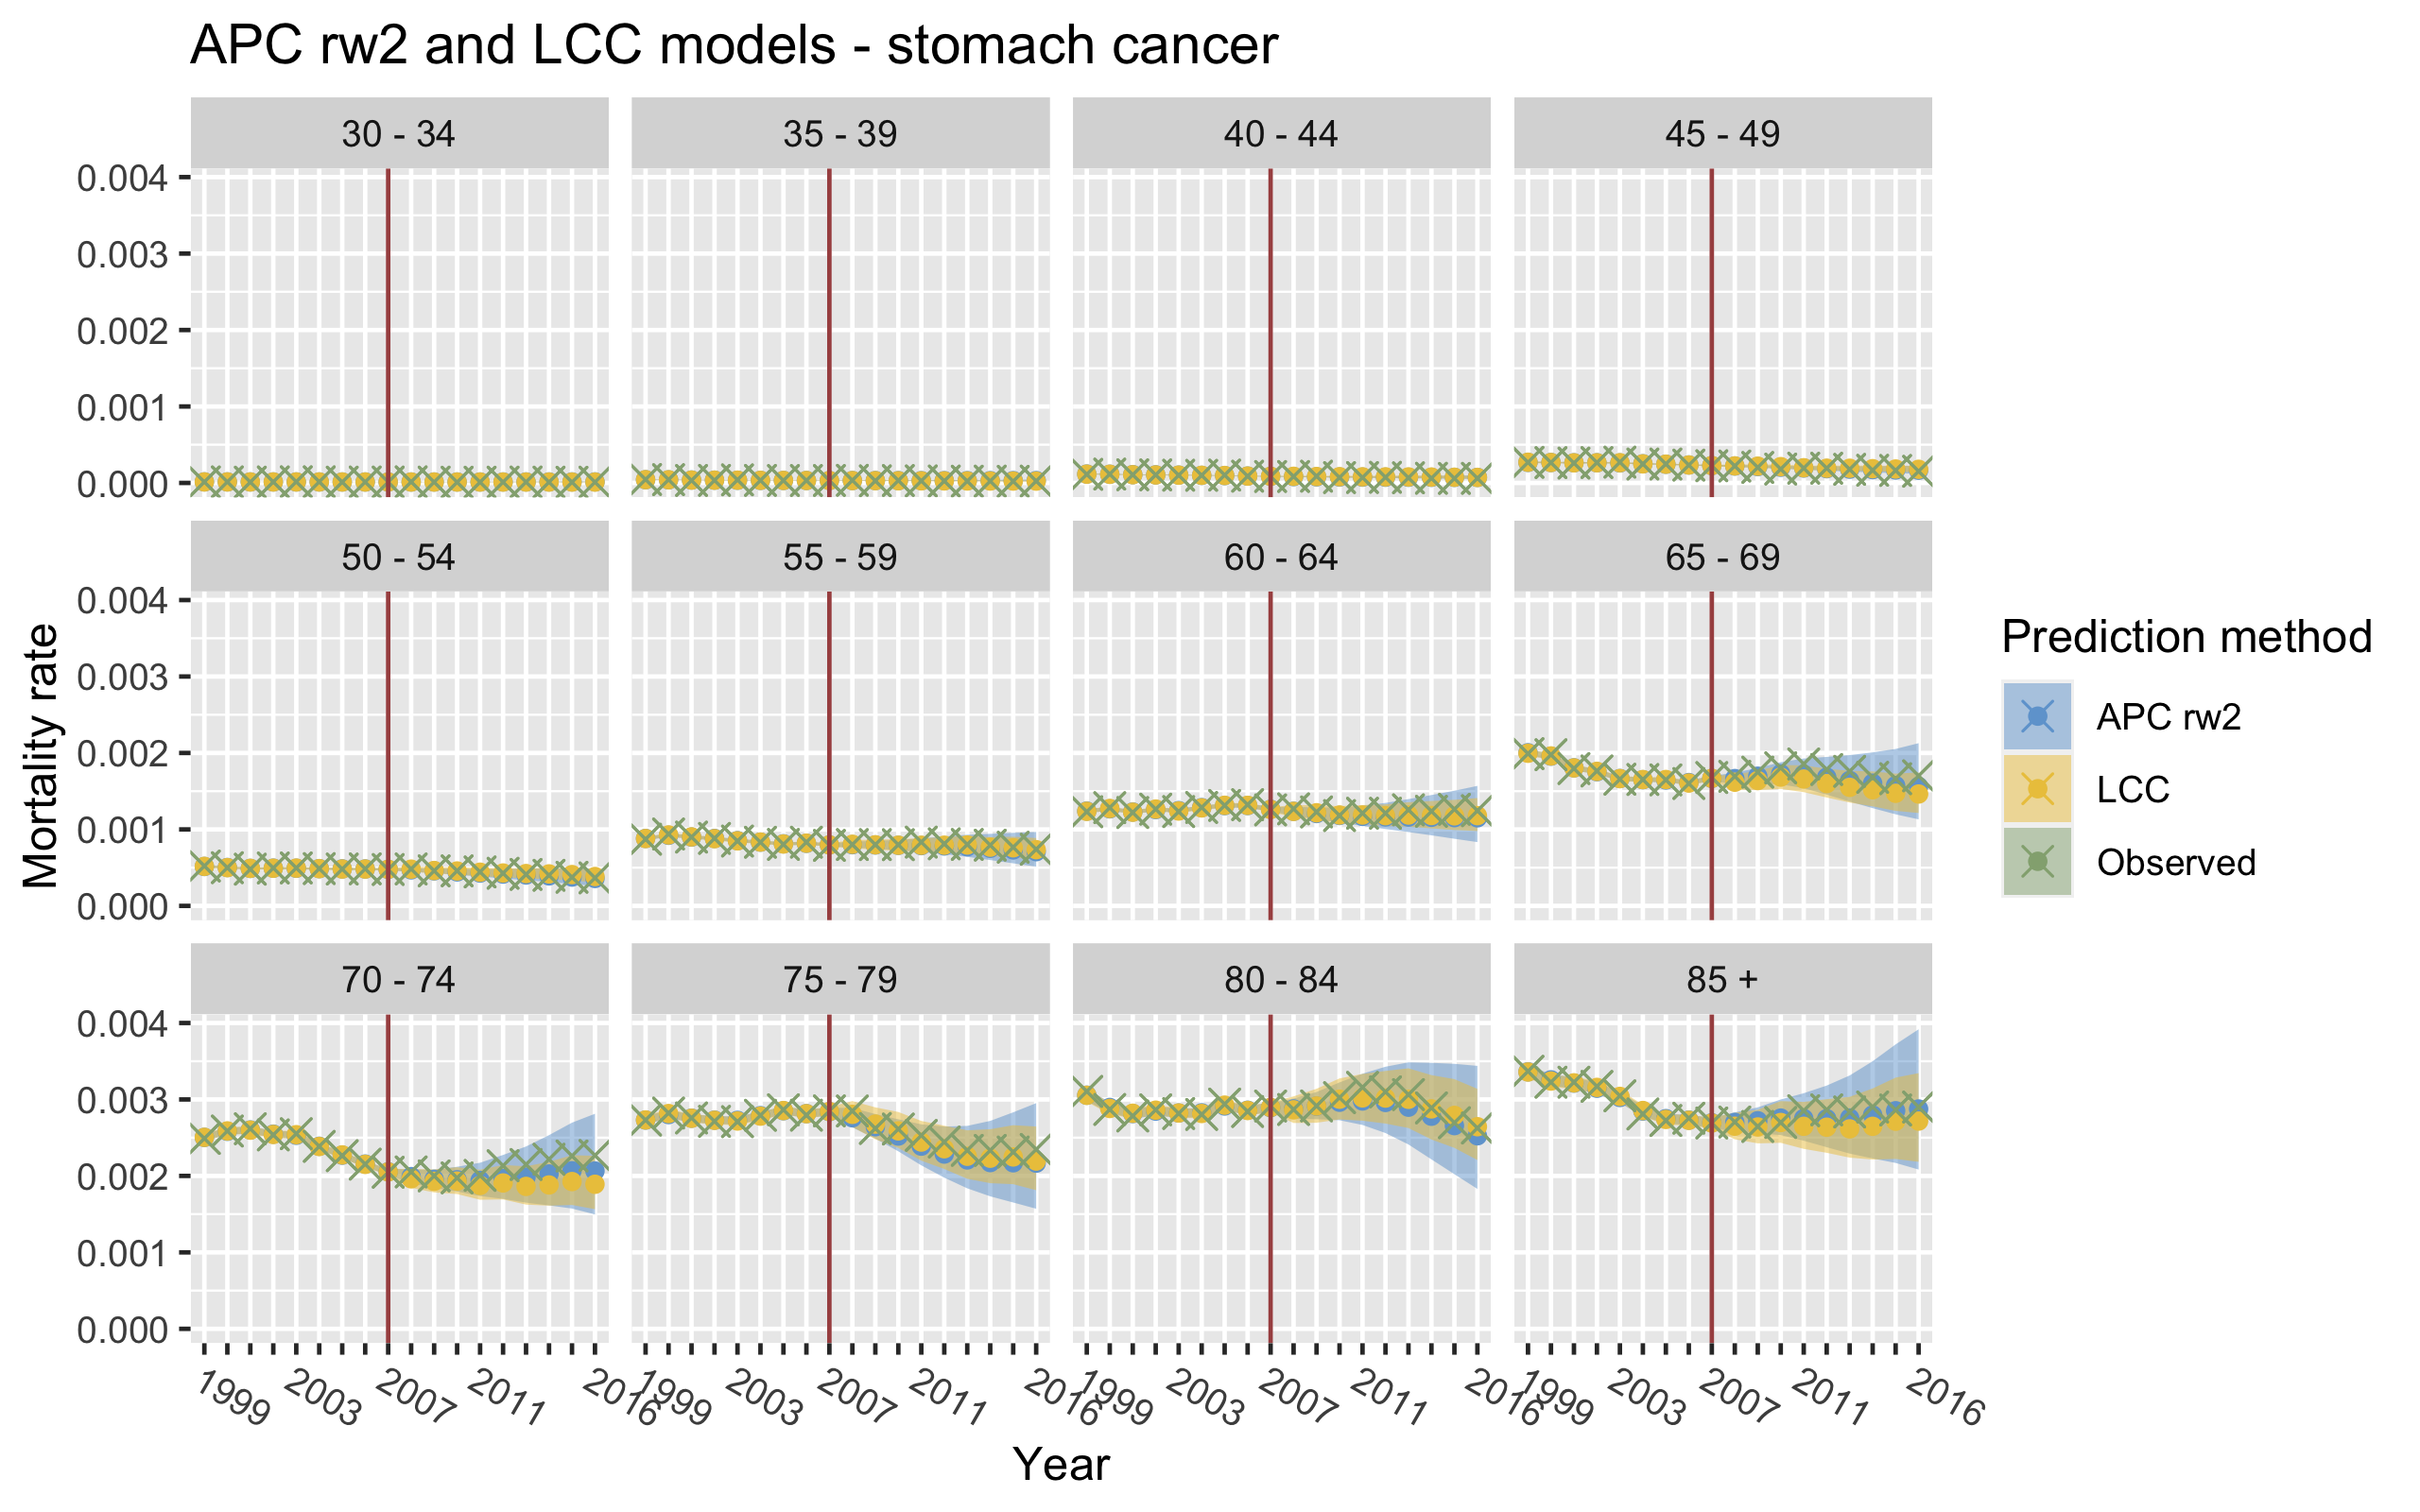
\includegraphics[width=\linewidth]{real-data/real-data-univariate/Figures/univariate-comparison-by-period-stomach.png}
        \label{fig:uv-comparison-stomach-bottom}
    \end{subfigure}
    \caption{The mean values and the 95\% confidence bounds of the predicted expected stomach cancer mortality rates produced by inference with the APC2- and the LCC-model on data of German stomach cancer (circles), together with the corresponding observed mortality rates $Y_{x,y}^{\text{stomach}}$ (crosses). The layout of the plots is similar to that of Figure \ref{fig:uv-LCC-lung}}
    \label{fig:uv-comparison-stomach}
\end{figure}

Figures \ref{fig:uv-comparison-lung} and \ref{fig:uv-comparison-stomach} display a comparison of the results from the Lee-Carter and the APC models with the lowest MDSS, the LCC- and the APC2-models, for lung and stomach cancer. For both cancer types, the APC2-model has a lower MDSS than the LCC-model does (see Tables \ref{tbl:uv-lung-5} and \ref{tbl:uv-stomach-5}), and we see from the plotted results that the APC2-model seems to be slightly more accurate than the LCC-model. We do, however note that the prediction intervals are narrower for the LCC-model predictions for both cancer types.

\newpage
\subsection{Prediction in the Multivariate Case}
\label{sec:pred-mv}

From the plots of the cancer mortality data in Section \ref{sec:GermanCancerData}, we observe a clear difference in male and female mortality rates, for both cancer types. The investigation of multivariate models with sex as a grouping factor, is then a natural next step in our analysis. We fit multivariate versions of Lee-Carter and APC models to the observed male and female cancer deaths, and use the male and female populations as the at-risk values. To avoid comparing too many different models, we test only the Lee-Carter and APC models that displayed the best MDSS in the univariate case, namely the LCC-model and the APC2-model (for both lung and stomach cancer). We use the approach described in Section \ref{sec:multivariateAPC} to obtain multivariate versions of the LCC- and APC2-model, namely keeping some of the random effects common across the sexes. It is not clear from the plots of the data which, if any, of the effects that should be kept common for male and female populations. Therefore, we find predictions using models with all combinations of common and separate age, period and cohort effects, and compare the results. We test the following versions of the LCC-model:
\begin{itemize}
    \item All common: $\eta_{x,t,s} = \mu_s + \alpha_x + \beta_x(\phi\cdot t + \kappa_t) + \gamma_k + \epsilon_{x,t,s}$
    \item Common age, period: $\eta_{x,t,s} = \mu_s + \alpha_x + \beta_x(\phi\cdot t + \kappa_t) + \gamma_{k,s} + \epsilon_{x,t,s}$
    \item Common age, cohort: $\eta_{x,t,s} = \mu_s + \alpha_x + \beta_x(\phi_s\cdot t + \kappa_{t,s}) + \gamma_{k} + \epsilon_{x,t,s}$
    \item Common period, cohort: $\eta_{x,t,s} = \mu_s + \alpha_{x,s} + \beta_{x,s}(\phi\cdot t + \kappa_t) + \gamma_{k} + \epsilon_{x,t,s}$
    \item Common age: $\eta_{x,t,s} = \mu_s + \alpha_x + \beta_x(\phi_s\cdot t + \kappa_{t,s}) + \gamma_{k,s} + \epsilon_{x,t,s}$
    \item Common period: $\eta_{x,t,s} = \mu_s + \alpha_{x,s} + \beta_{x,s}(\phi\cdot t + \kappa_{t}) + \gamma_{k,s} + \epsilon_{x,t,s}$
    \item Common cohort: $\eta_{x,t,s} = \mu_s + \alpha_{x,s} + \beta_{x,s}(\phi_s\cdot t + \kappa_{t,s}) + \gamma_{k} + \epsilon_{x,t,s}$
    \item No common: $\eta_{x,t,s} = \mu_s + \alpha_{x,s} + \beta_{x,s}(\phi_s\cdot t + \kappa_{t,s}) + \gamma_{k,s} + \epsilon_{x,t,s}$,
\end{itemize}
where $s \in \{0 = male, 1 = female\}$. Note that the "No common" version of the model is equivalent to fitting two separate univariate LCC-models to the male and female parts of the data. Note that we always keep $\beta_x$ common for the sexes in the models where we keep $\alpha_x$ common, and vice versa for the models where $\alpha_x$ is modelled separately for each sex. We could have included all versions where e.g. $\beta_x$ is modelled as a common effect and $\alpha_x$ is modelled separately, but we do not do this simply to reduce the number of models that we need to compare. For the APC2-model, we test the following multivariate versions:
\begin{itemize}
    \item APC: $\eta_{x,t,s}= \mu_{s} + \rho_x + \phi_t + \psi_k + \epsilon_{x,t,s}$ 
    \item APc: $\eta_{x,t,s}= \mu_{s} + \rho_x + \phi_t + \psi_{k,s} + \epsilon_{x,t,s}$ 
    \item ApC: $\eta_{x,t,s}= \mu_{s} + \rho_x + \phi_{t,s} + \psi_{k} + \epsilon_{x,t,s}$ 
    \item aPC: $\eta_{x,t,s}= \mu_{s} + \rho_{x,s} + \phi_{t} + \psi_{k} + \epsilon_{x,t,s}$ 
    \item aPc: $\eta_{x,t,s}= \mu_{s} + \rho_{x,s} + \phi_{t} + \psi_{k,s} + \epsilon_{x,t,s}$ 
    \item apC: $\eta_{x,t,s}= \mu_{s} + \rho_{x,s} + \phi_{t, s} + \psi_{k} + \epsilon_{x,t,s}$ 
    \item apc: $\eta_{x,t,s}= \mu_{s} + \rho_{x,s} + \phi_{t, s} + \psi_{k, s} + \epsilon_{x,t,s}$,
\end{itemize}
where $s \in \{0 = male, 1 = female\}$. Following \textcite{rieblerHeld2010}, we name the different versions of the APC2-model by capital letter for the common effects and shared letters for the male- and female-specific effects.  
% \newpar To fit these multivariate models with \inlabru, we need to change the implementation of the prediction compared to the implementation of the univariate models. To implement the multivariate models, we use two likelihoods, one for each sex. For the effects that will not be common for male and females, we include two identical model components, but named differently. These are included in one likelihood each. For the effects that are kept common, we only include one model component, which is used in both likelihoods. We only include male data in the male likelihood and female data in the female likelihood. Below, the part of the code used to produce predictions for the aPc-model is shown:

% \begin{verbatim}
% comp.aPc = ~ -1 + 
%   mu(s, model = "iid", hyper = list(prec = list(fixed = TRUE,
%     initial = log(0.001)))) +
%   rho0(x, model = "rw2", values = unique(stomach.cancer$x), constr = TRUE,
%     hyper = pc.prior, scale.model = TRUE) + 
%   rho1(x, model = "rw2", values = unique(stomach.cancer$x), constr = TRUE,
%     hyper = pc.prior, scale.model = TRUE) + 
%   phi(t, model = "rw2", values = unique(stomach.cancer$t), constr = TRUE,
%     hyper = pc.prior, scale.model = TRUE) + 
%   psi0(k, model = "rw2", values = unique(stomach.cancer$k), constr = TRUE,
%     hyper = pc.prior, scale.model = TRUE) + 
%   psi1(k, model = "rw2", values = unique(stomach.cancer$k), constr = TRUE,
%     hyper = pc.prior, scale.model = TRUE) + 
%   epsilon(xts, model = "iid", hyper = pc.prior)

% # define two different likelihoods and formulas, for male (0) and female (1):
% form.aPc.0 = cases ~ -1 + mu + rho0 + phi + psi0 + epsilon
% likelihood.aPc.0 = like(formula = form.aPc.0, family = "poisson",
%     data = /*data frame containing male mortality cases*/,
%     E = /*data frame containing male population*/)

% form.aPc.1 = cases ~ -1 + mu + rho1 + phi + psi1 + epsilon
% likelihood.aPc.1 = like(formula = form.aPc.1, family = "poisson",
%     data = /*data frame containing female mortality cases*/,
%     E = /*data frame containing female population*/)

% res.aPc = bru(components = comp.aPc,
%               likelihood.aPc.0,
%               likelihood.aPc.1,
%               options = list(/*Desired options*/
%               )) 
% \end{verbatim}
\newpar We perform the preciction analysis in the same way as for the univariate case, using the years 1999-2007 to fit the models and then predict the mortality for years 2008-2016. We again exclude the predictions for ages younger than 30 years old ($x \leq 5$) when we calculate the score statistics. The code used to produce the results in this section can be found at the \texttt{Github} repository under \path{/real-data/real-data-multivariate/Lung_cancer} and \path{/real-data/real-data-multivariate/Stomach_cancer}. We present the results for lung and stomach cancer, respectively, in the following two sections.

\import{}{Report/4-Real-data/mv-lung.tex}

\import{}{Report/4-Real-data/mv-stomach.tex}

\newpage
\subsection{Sensitivity analysis of hyperpriors}
Throughout our analysis, we have used the same informative priors for all hyperparameters, for both the Lee-Carter models and the APC-models, without considering the effect this choice have on the prediction results. To investigate how predictions with different hyperpriors could change our results, we run the analysis using the aPc-model with three different prior distributions, namely PC-priors with the parameters
\begin{equation}
    \begin{aligned}
        \mathbb{P}(1/\sqrt{\tau} > 1) & = 0.05 \\
        \mathbb{P}(1/\sqrt{\tau} > 3) & = 0.05 \\
        \mathbb{P}(1/\sqrt{\tau} > 1) & = 0.95.
    \end{aligned}
\end{equation}
The score statistics for the different runs are presented in Tables \ref{tbl:mv-sensitivity-lung} and \ref{tbl:mv-sensitivity-stomach}. We observe that the predictions using the different hyperpriors have very similar score statistics, an indication that our choice of hyperpriors did not significantly influence the result. 

% \begin{figure}[h!]
%     \centering
%     \begin{subfigure}[b]{.45\linewidth}
%         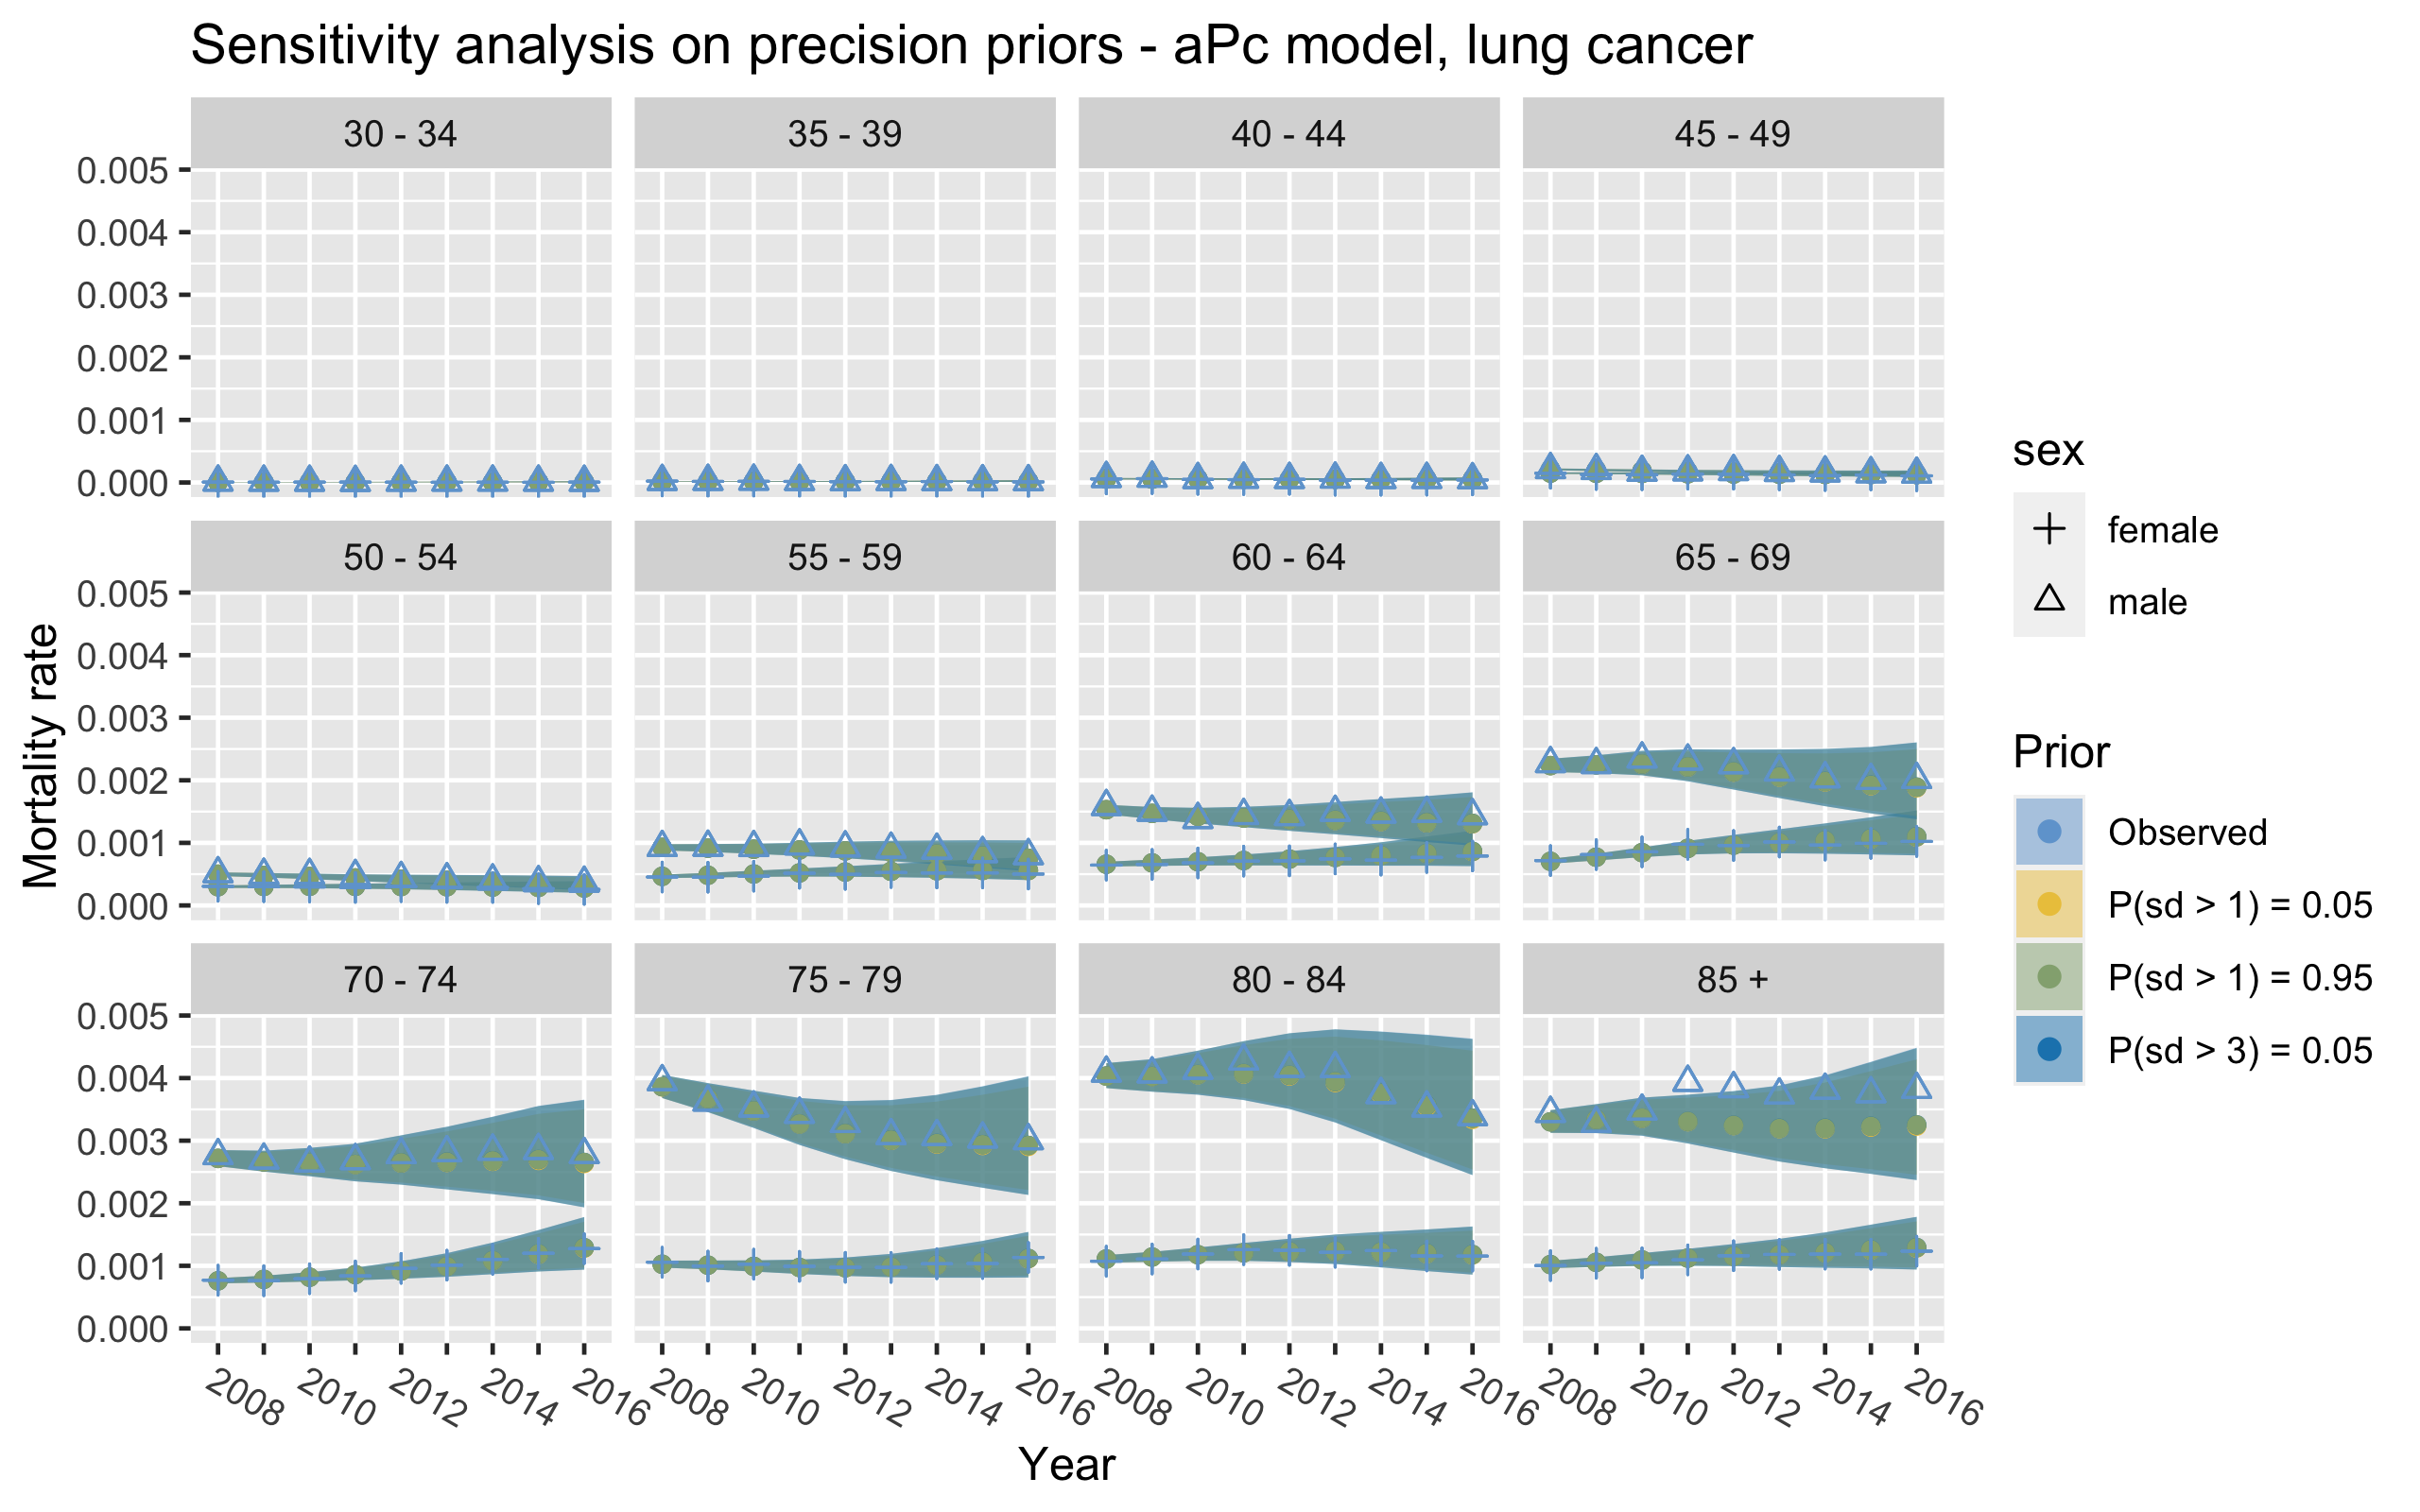
\includegraphics[width=\linewidth]{real-data/real-data-multivariate/Figures/sensitivity-analysis-aPc-by-period-lung.png}
%     \end{subfigure}
%     \begin{subfigure}[b]{.45\linewidth}
%         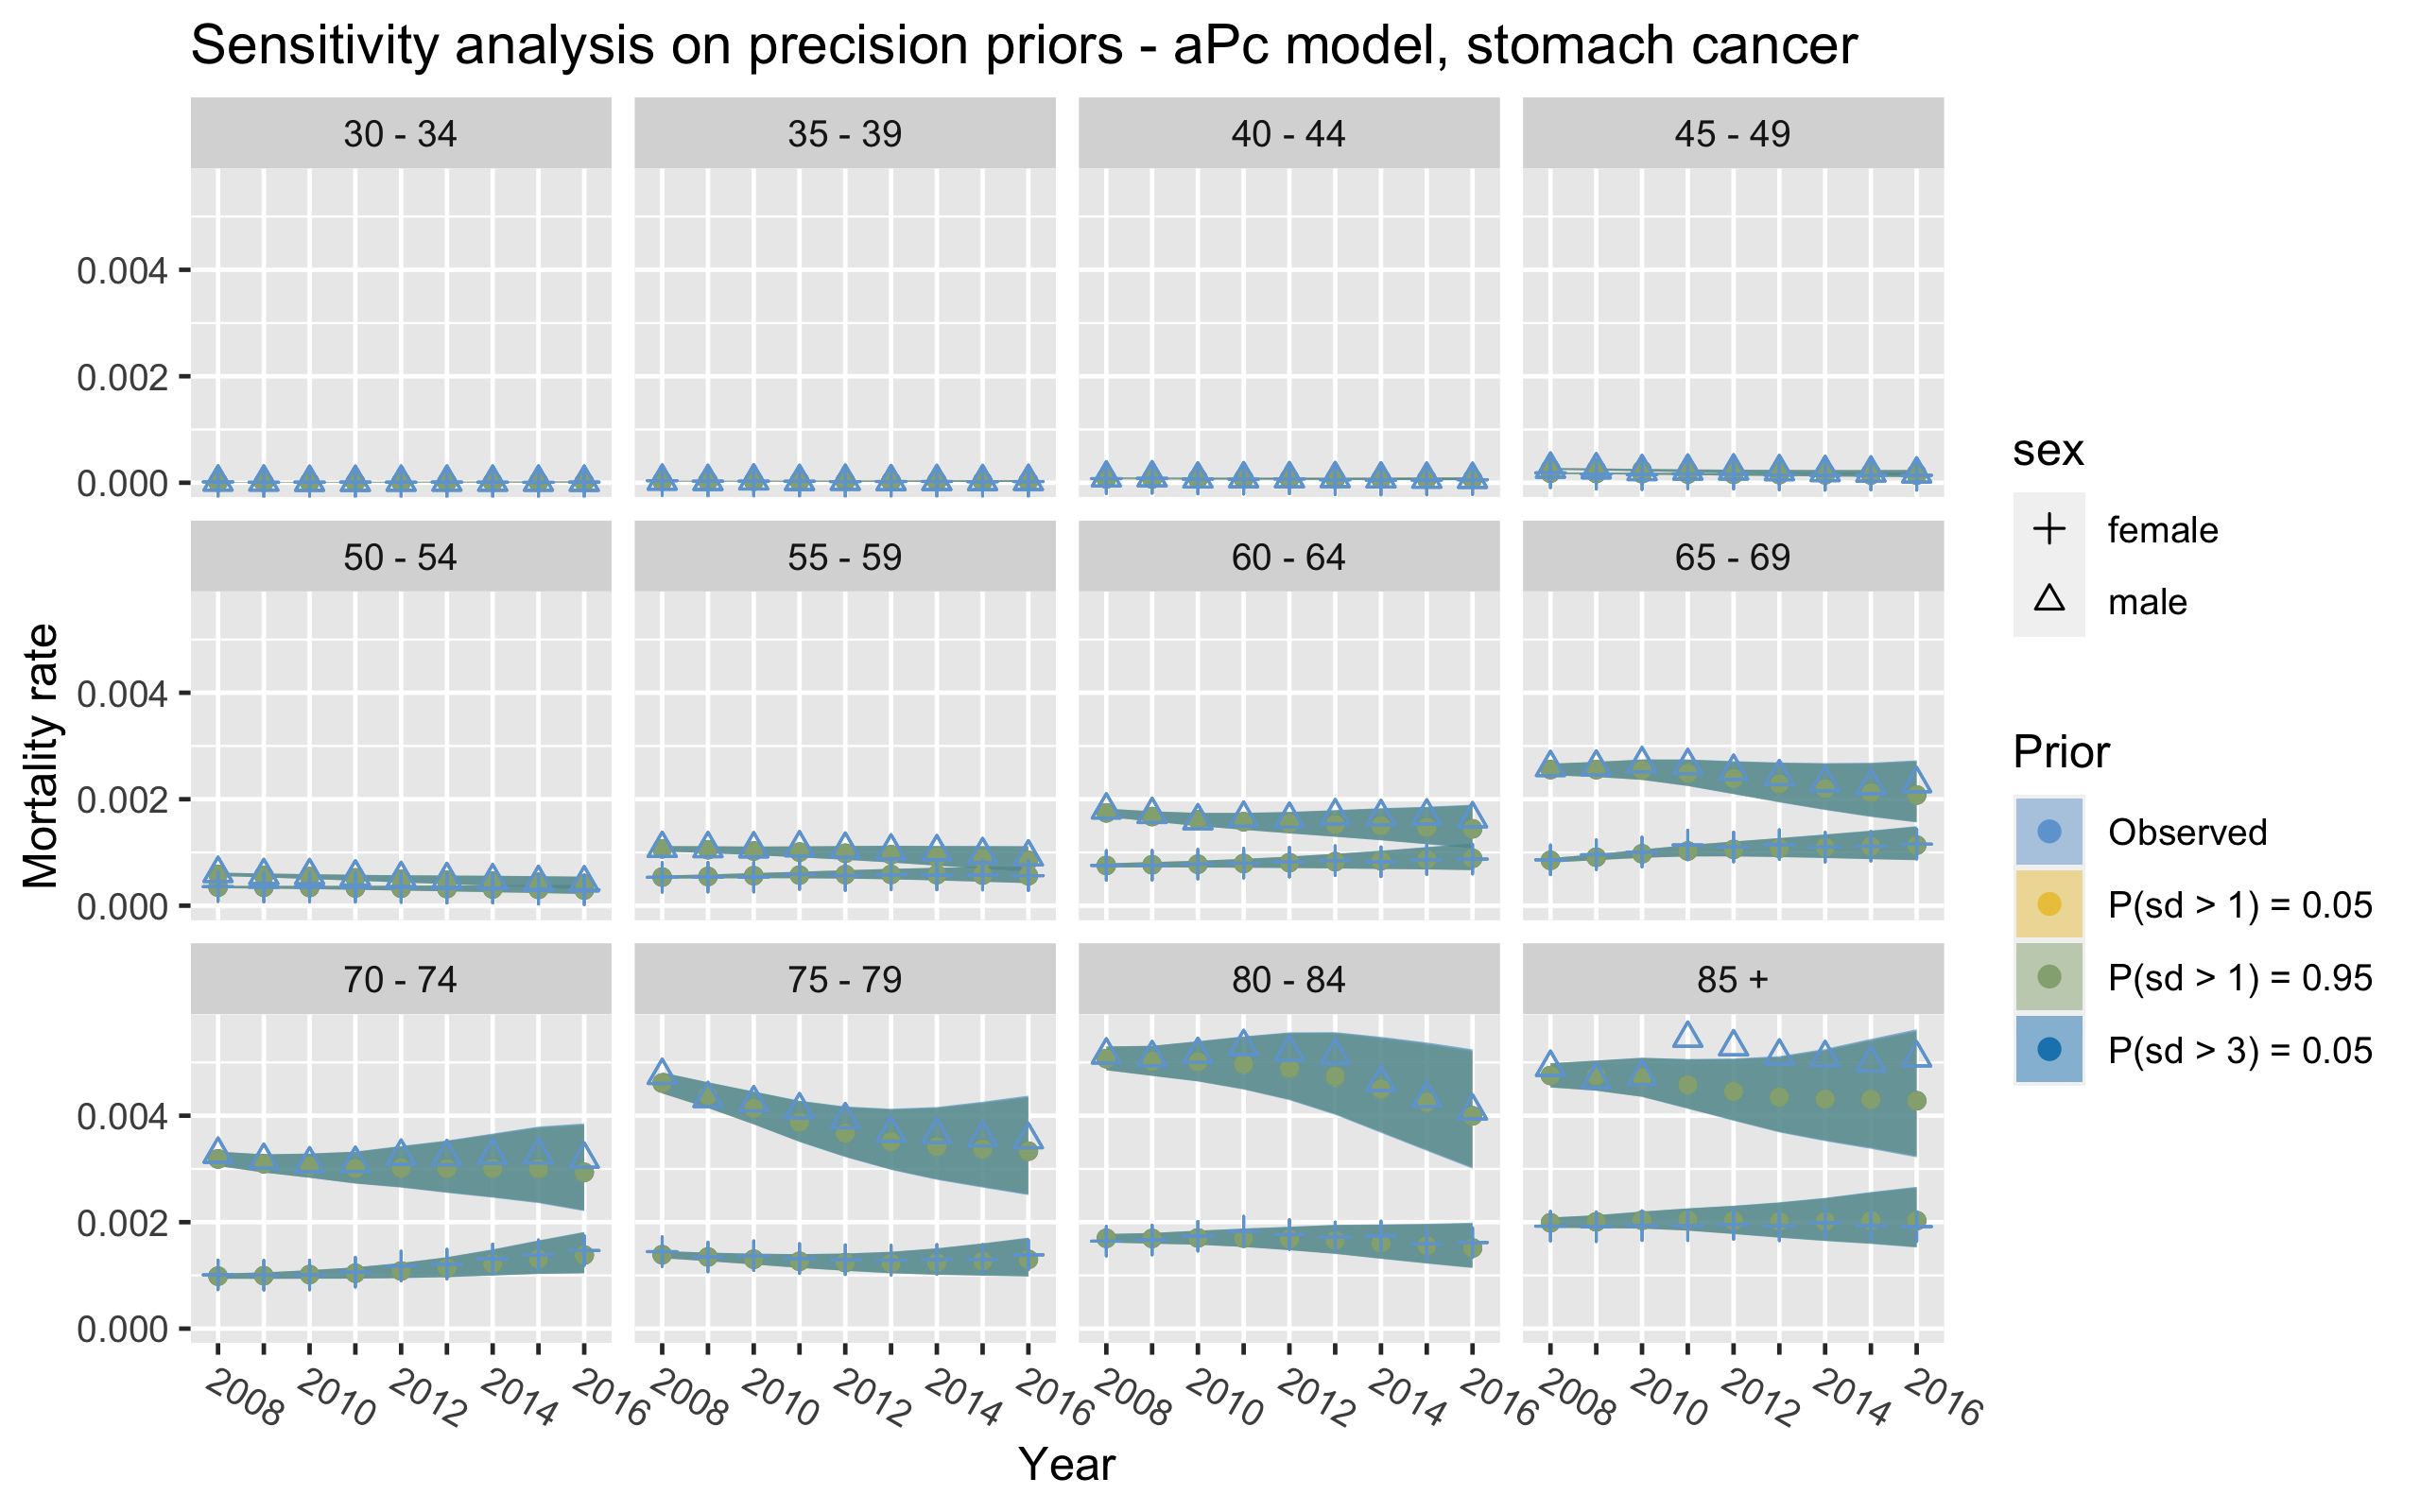
\includegraphics[width=\linewidth]{real-data/real-data-multivariate/Figures/sensitivity-analysis-aPc-by-period-stomach.png}
%     \end{subfigure}
%     \caption{Results from sensitivity analysis of the model that displayed the best predctive performance for lung cancer, the aPc-model (left), and stomach cancer, also the aPc model (right). \textcolor{myDarkGreen}{Remove this image if we have the table?}}
%     \label{fig:mv-sensitivity}
% \end{figure}

\begin{table}
    \begin{center}
        \begin{tabular}{l |c c c }
        Model & MSE &   MDSS & Contained 95\%-interval\\
        \hline
        P(sd > 1) = 0.05 & 0.00000002.535e-8 & -19.36    & 0.9120\\
        P(sd > 1) = 0.95 & 0.00000002.518e-8 & -19.37    & 0.9120\\
        P(sd > 3) = 0.05 & 0.00000002519 & -19.37    & 0.9120\\
        \end{tabular}
    \caption{Results from sensitivity analysis, stomach cancer data.}\label{tbl:mv-sensitivity-stomach}
    \end{center}
\end{table}

\begin{table}
    \begin{center}
        \begin{tabular}{l |c c c }
        Model & MSE &   MDSS & Contained 95\%-interval\\
        \hline
        P(sd > 1) = 0.05 & 1.238e-8 & -19.83    & 0.9028 \\
        P(sd > 1) = 0.95 & 1.189e-8 & -19.74    & 0.9028 \\
        P(sd > 3) = 0.05 & 1.182e-8 & -19.73    & 0.9028 \\
        \end{tabular}
    \caption{Results from sensitivity analysis, lung cancer data}\label{tbl:mv-sensitivity-lung}
    \end{center}
\end{table}

\newpage
\section{Closing remarks / further work}
\label{sec:closingRemarks}
\textcolor{myDarkBlue}{Not finished.}
\begin{itemize}
    \item Investigate periodicity in $\gamma_k$. Could it be avoided using random walk-2 priors? 
    \item For some models, \inlabru does not converge - further investigation? 
    \item Cohort effects - what are trends and what results from identifiability? 
    
    \item In general - identifiability issues. Du har ikke snakket noe om hvordan APC1 of APC2 solve identifiability problem differently. 
\end{itemize}
We ahve shown that Bayesian inference using the \INLA methodology through the \inlabru method is feasible for a Poisson extension of the Lee-Carter model as well as for a Possion exension of the Lee-Carter model with a cohort effect. Before the introduction of the \inlabru method by \textcite{BachlLindgren2019}, this was not possible. We have shown this for the general case, using synthetic data. In this phase of the study, described in Section \ref{sec:SyntheticData}, we have shown that the \inlabru method, with some exceptions, enabled correct estimation of both the simulated predictor and the simulated random effects in Lee-Carter models. We have also displayed the ability for \inlabru to make Bayesian inference in the specific case of German lung and stomach cancer mortality rates. In this phase of the research, described in Section \ref{sec:real-data}, we have shown that we could use the \inlabru method to correctly estimate lung and stomach cancer mortality rates with both Lee-Carter methods. We were also able to obtain and assess predictions of cancer mortality produced using \inlabru for both models, and observed that the prediction quality of the cohort-extended Lee-Carter model was better for both cancer types. Finally, we used the \inlabru method to fit multivariate versions of the Lee-Carter models to obtain predictions of male and female cancer mortality, and we compared the prediction quality of the different models. We note that our simple trial-and-error approach in this stage of the research was to a large degree made feasible in our limited time scope by the computational power of the \inla methodology. Throughout the part of the research involving real cancer data, we compared the prediction results of the Lee-Carter models to prediction results on the same data by different versions of the commonly used Age-Period-Cohort (APC) model. We have shown that the predictive qualities of the cohort-extended Lee-Carter models and the APC models are quite similar, but that the APC-models receive overall slightly better prediction scores while the Lee-Carter models seem to display narrower prediction intervals.     

\newpar Our research can be extended in several ways. The estimated cohort effects for the Lee-Carter models display periodical tendencies similar to those observed for cohort-related identifiability issues in APC-models (described by e.g. \textcite{RieblerThesis2010}). We have not investigated this and its potential effects on the predictive results, something that would be interesting to know more about. 

\newpar Another result that we leave unexplored in this paper is the inability of \inlabru to converge for some versions of the Lee-Carter models. A further analysis of the properties of the data-model combinations that trigger this response would be interesting. 

